\chapter{The SLIM5 Project}
\label{chap:SLIM5}
In this Chapter the SLIM5 R\&D project will be presented. After a short summary of the project 
motivations, goals and timeline (Section~\ref{sec:SLIM5Project}), the Physics motivations of 
and the tracker requirements for SuperB and ILC will be briefly discussed in Section~\ref{sec:HLExp}. 
The pixel  (Section~\ref{sec:Apsel4D}) and strip (Section~\ref{sec:Striplets}) 
detector prototypes developed 
within the SLIM5 project will be presented. In Section~\ref{sec:SLIM5Results} the results 
in~\cite{BETTARINI2010942,BOMBEN2010159,NERI2010195} will be discussed. 
A special Section (~\ref{sec:striplets_res}) is devoted to the spatial resolution of the striplets. 
Wrap up of the SLIM5 project will be finally outlined in Section~\ref{sec:Slim5Summary}.


\section{The Project}
\label{sec:SLIM5Project}
The SLIM5 project~\cite{SLIM5:proj} aimed at advancing the state-of-the-art in the development of thin 
tracking systems to be applied in High-Energy Physics. The project was financed for three years
 (2006-2008) by INFN - National Scientific Committee 5~\cite{INFN_V} and involved several 
 italian research institutes. 
 
 The SLIM5 collaboration worked on developing tracking systems for experiments at 
 high luminosity flavour 
 factories, like the proposed SuperB (\cite{Baszczyk:2013xua}) and linear colliders. The goal was to deliver thin silicon tracking detectors with possibility 
 of self-triggering thanks to the combination of data-driven data acquisition and pattern matching 
 algorithm with very low latency.
Let's know see the required performance for such detectors. 

\section{Tracking and Vertexing Requirements for SuperB and ILC Experiments}
\label{sec:HLExp}
Experiments at high luminosity colliders have to accomplish a high precision measurements 
exploiting at maximum the large dataset they are expected to integrate. 
This means that the experiments have to be very efficient and show excellent performance, 
even in presence of a very intense particle rate; this is particularly true for the tracking and 
vertexing detectors, which are the closest to the beams interaction point. It has also to be stressed 
that with sub-optimal tracking and vertexing performance there's no physics case for such 
experiments; hence the tracking and vertexing detectors are the crucial parts of experiments at 
high luminosity colliders.

We now review quickly some physics cases for SuperB and ILC and the related constraints on 
tracking detectors.
\subsection{SuperB}

The SuperB project~\cite{Baszczyk:2013xua} was the proposal of a super flavour $\epem$ factory operating at the 
 center-of-mass energy of the \Y4S, capable of an instantaneous 
 luminosity of  $10^{36}\cms$, with the goal of integrating 50--75~\invab.

The SuperB physics program was to 
\begin{itemize}
\item[a)]determine the flavor structure of whatever New Physics discovered at the LHC, 
using the information on rare $b$, $c$, and $\tau$ decays, and on \CP
violation in $b$ and $c$ quark decays, or, if  signatures of New Physics were not observed at the LHC,
then
\item[b)]  exploit the excellent sensitivity provided at the luminosity frontier by
a super $B$ factory, to
observing New Physics at mass scales up to 10~\tev or more through
observation of rare processes involving $B$ and $D$ mesons and studies
of lepton flavour violation in $\tau$ decays.
\end{itemize}

The SuperB detector concept was based on the \babar\ detector~\cite{AUBERT20021}, with
those modifications required to operate at a luminosity of $10^{36}\cms$
or more, and with a reduced center-of-mass boost.
Higher luminosity and machine-related backgrounds, as well
as the need to  improve detector hermeticity
and performance, required significant R\&D
to be able to implement this upgrade.


The SuperB Vertex Tracker (SVT) was intended to be an evolution of the \babar\ 
SVT; see Figure~\ref{fig:svt} for a comparison. The main difference was the extra layer, Layer0, 
at a radius of 1.5~cm.

\begin{figure}
\centering
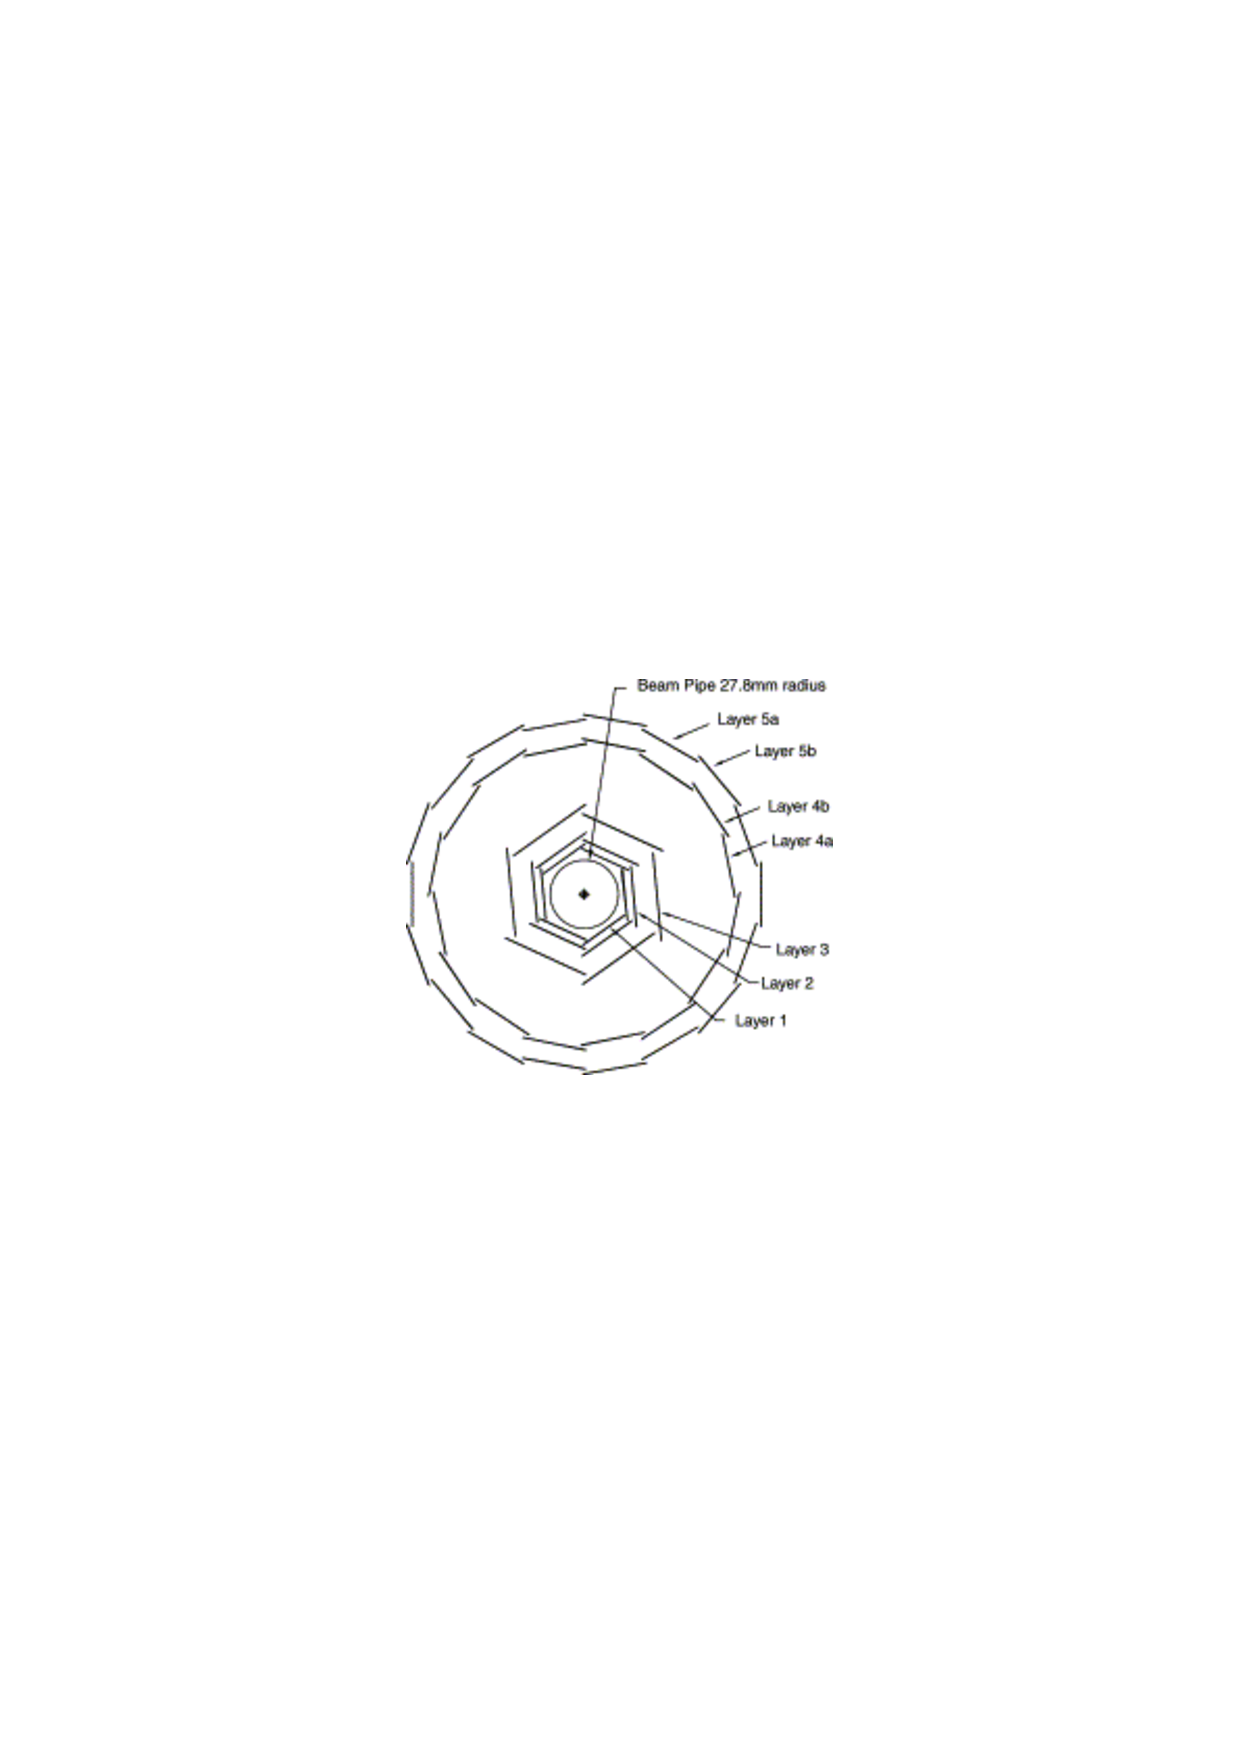
\includegraphics[width=0.45\textwidth]{miniSVT.pdf}
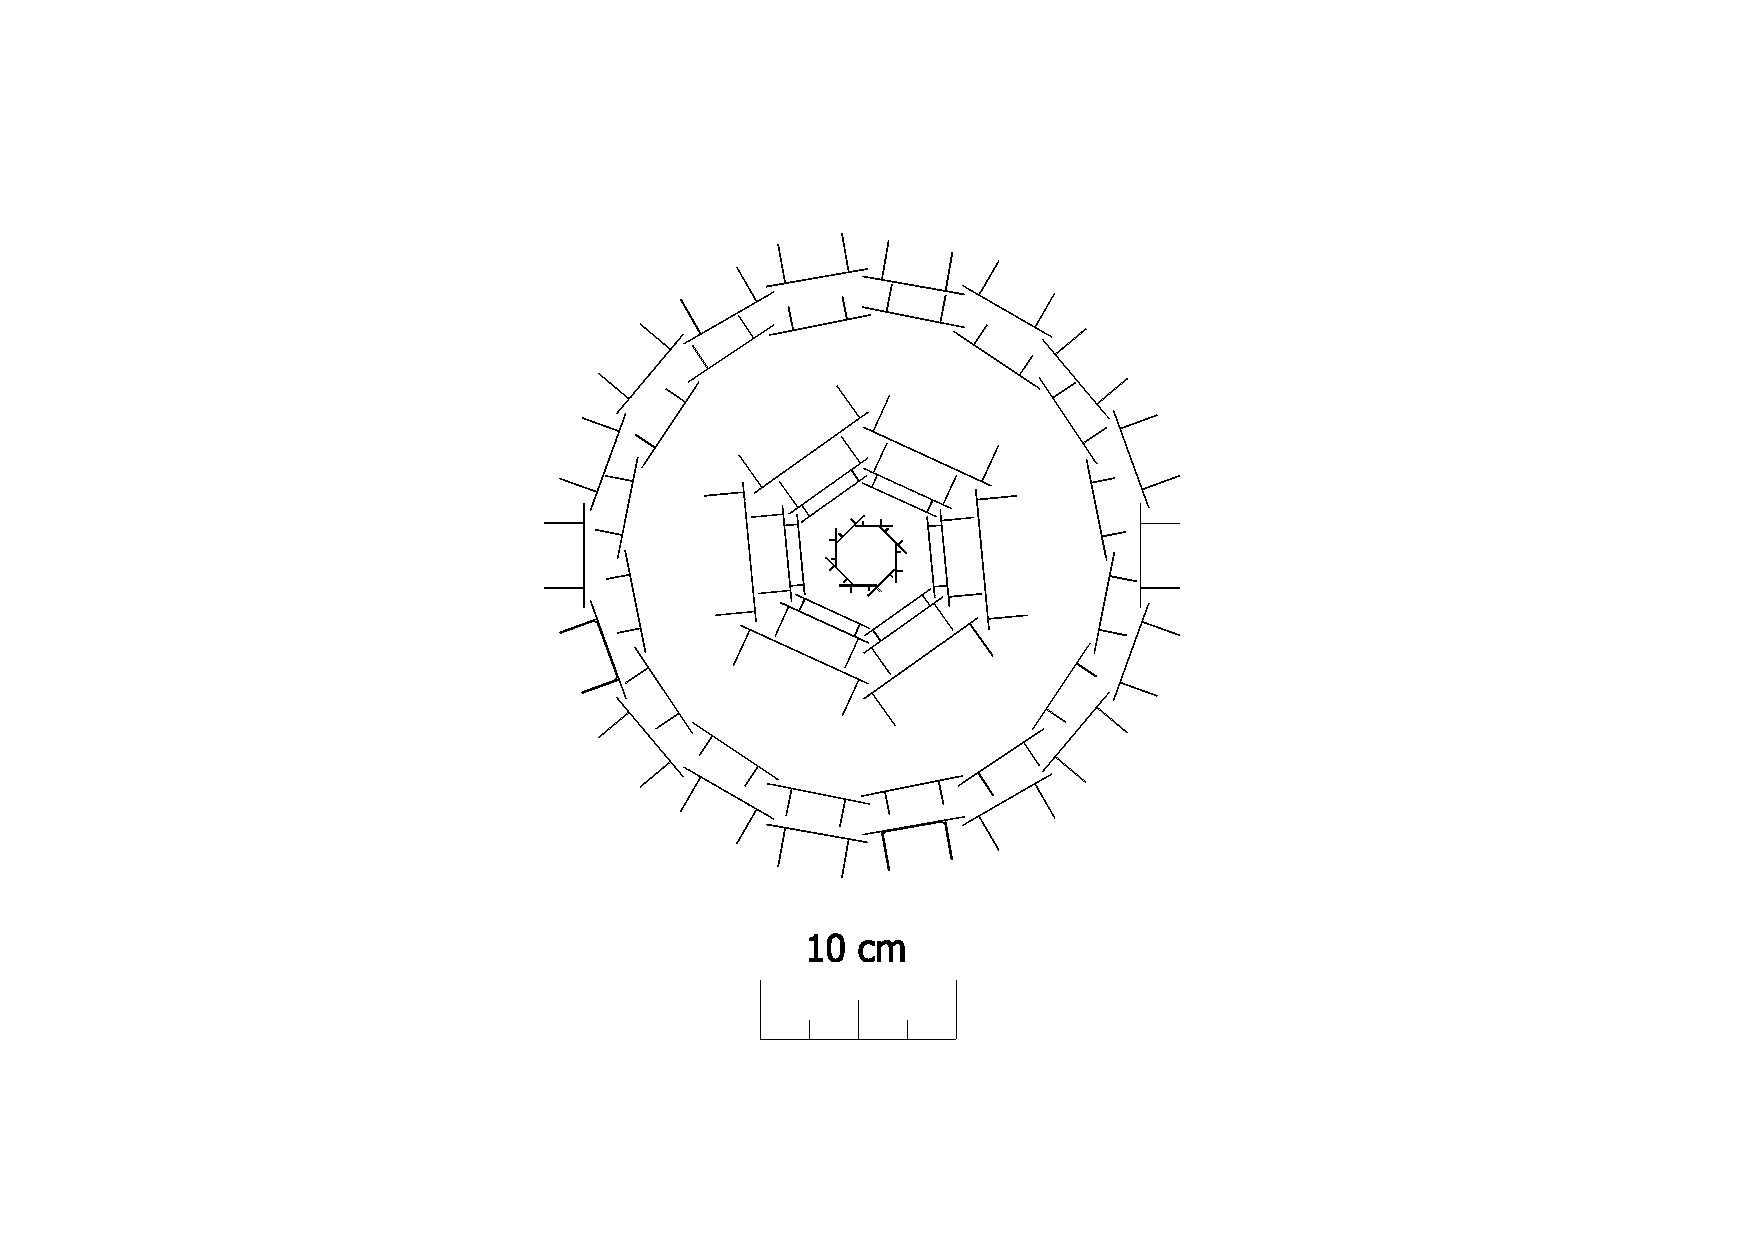
\includegraphics[width=0.45\textwidth]{miniSuperBSVT.pdf}
\caption{\label{fig:svt} (left)Schematic view of \babar\ SVT: tranverse section. (After~\cite{AUBERT20021}) The external radius is 144 mm. (right) Cross section of the SuperB SVT. (After~\cite{Baszczyk:2013xua}) }
\end{figure}


Precise vertex information, primarily extracted from precise position measurements near the 
interaction point (IP) by the SVT  is crucial to the measurement of time-dependent \CP asymmetries 
in \Bz decays, which was the  key element of the SuperB physics program. As in \babar, the SuperB 
had to be able to provide efficient and accurate tracking for  charged particles with transverse 
momenta lower than 100~MeV/c, which cannot reach the tracking Drift Chamber.

SuperB SVT had to be capable of maintaining adequate performance for time-dependent 
measurements
 in the presence of a lower boost of the center-of-mass (CM) frame
($\beta\gamma = 0.24$ compared to $\beta\gamma = 0.55$ of \babar) and much higher background,
mainly related to the increased instantaneous luminosity of about a factor of 100 larger than \babar.

The planned beam pipe featured a reduced radius of about $1.0~\cm$  which allows the positioning of 
Layer0 at
the desired average radius of about $1.5~\cm$. The additional  (with respect to \babar\ SVT) 
 Layer0 measurement,
along with the low radial material budget of the beam pipe ($0.42\%~X_0$)
and of Layer0 ($0.45\%~X_0$ with the striplet option - see Section~\ref{sec:Striplets}),
was crucial for improving the decay vertex reconstruction of the \B mesons and
 obtaining adequate proper-time resolution for time-dependent \CP violation measurements.

Physics simulations for the $B\to\pip\pim$ decay channel showed that to retain or improve the vertexing performance of the \babar\ SVT in the SuperB environment the following ingredients were necessary: the use of high granularity pixels (50~$\mu$m $\times$50~$\mu$m pitch), going indeed closer to the beam pipe and very low material budget~\cite{RIZZO2010585}. Results are shown in 
Figure~\ref{fig:bpipi}. 

\begin{figure}
\centering
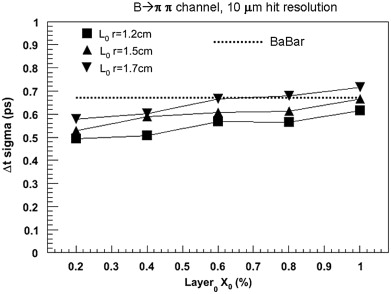
\includegraphics[width=0.45\textwidth]{bpipi}
\caption{\label{fig:bpipi} Resolution on the proper time difference of the two B mesons for the nominal SuperB boost, for different Layer0 radii, as a function of Layer0 thickness (in $X_0$ \%). The BaBar resolution for the same decay channel, is shown with a dashed line. (After~\cite{RIZZO2010585})}
\end{figure}

In summary, for the SuperB physics program a silicon tracker detector was needed with the 
capability to assure a space-point resolution of 10~$\mu$m, with a material budget below 
1\% of $X_0$, able to measure tracks with $p_T$ lower then 100~MeV/c. The real detector 
would have had to withstand a particle rate of 100~MHz/cm$^2$, mainly due to machine 
background.

\subsection{ILC}

The International Linear Collider (ILC) is a proposed $\epem$ collider. Over the years the project 
evolved and now it features a machine capable of tuning its center of mass energy in the range of 
$\sqrt{s}=250-550$~GeV, with an option for 1~TeV~\cite{ILCTDR}.  
In 2009, two detector projects (ILD \& SiD) provided a Letter Of Intent (LOI)~\cite{ILDLOI,SIDLOI}.

The ILC physics goals cover a wide and ambitious program including top quark physics, electroweak 
precision measurements, direct and indirect searches beyond the Standard Model (BSM) like SUSY, 
dark matter searches, exotic searches, etc., and a complete and extensive Higgs physics program 
covering mass, couplings to fermions and bosons, quantum numbers and total width 
measurements.  The expected level of precision for the majority of them will 
reach the percent level and will allow probing physics BSM~\cite{ILCVertexing2016}.

To accomplish this ambitious physics program stringent requirements are imposed on tracking and 
vertexing performances; these requirements didn't change much over a 
decade~\cite{ILCVertexing2007,ILCVertexing2016}. 
The  figure of merit of the future ILC vertex detector  is the impact parameter (ip) resolution which is 
expected to be:

\begin{equation}
\sigma_{ip}=5\,\mu{\rm m}\oplus\dfrac{10}{p\beta(\sin\theta)^{3/2}}\,\,\mu{\rm m\, GeV/c}
\label{eq:ILCipres}
\end{equation}

This condition demands then for: a space-point resolution of about 3~$\mu$m (hence a pitch of less 
than 20~$\mu$m; a material budget per layer of about 0.1\% of $X_0$; capabilities of performant    
tracking	down to $p_T$ of 100~MeV/c and even less.

The vertexing systems proposed by the two concept groups are both built around a central 
part based on pixel detectors; a comparison of ILD and SiD proposed solutions is presented in 
Figure~\ref{fig:ILC_concepts}. SiD features 5 pixel barrel layers and a total of 7 pixel disk layers 
per side; ILD plans for 3 double sided ladders plus , a system of pixels and strips disks  in the forward 
region.

\begin{figure}
\centering
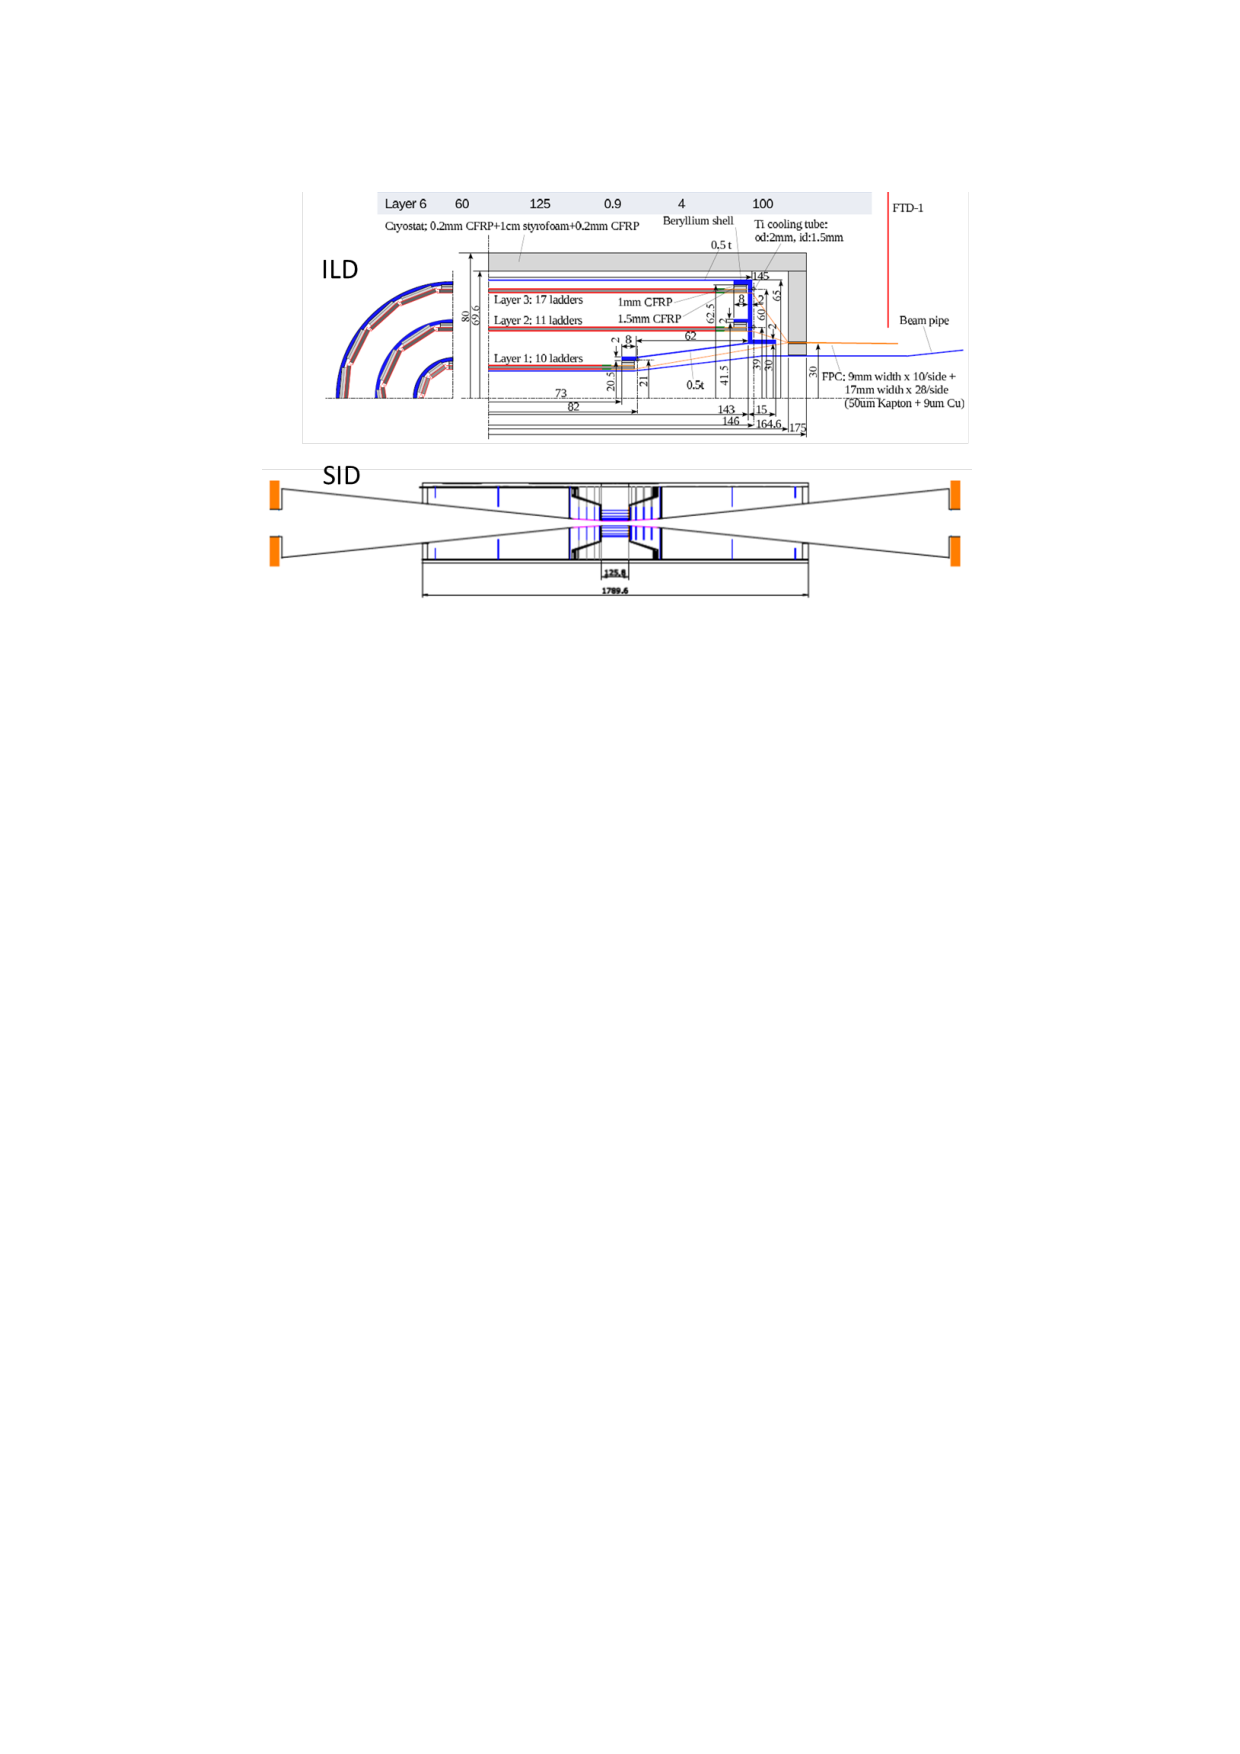
\includegraphics[width=0.5\textwidth]{ILC_concepts.pdf}
\caption{\label{fig:ILC_concepts}ILD and SiD schemes of the vertex detector (After~\cite{ILCVertexing2016})}
\end{figure}

For both vertexing detectors pixels with integrated readout (at least partial) are promising solutions, 
like CMOS MAPS, DEPFET, etc. They will assure the needed small pitch and the low material 
budget (example:~\cite{mimosa26}). 

In Summary, for the experiment at the future ILC a vertex detector with a space point resolution of 
3~$\mu$m, a material budget per layer of about 0.1\% of $X_0$ and the possibility  of    
tracking down to $p_T$ of 100~MeV/c and even less is needed.



\section{The CMOS MAPS Apsel4D}
\label{sec:Apsel4D}

As said in the introduction to this Chapter, within the SLIM5 project both pixel and strip detector
prototypes were developed. We now review the salient features of the pixel 
detector prototype, the Apsel4D. More details can be found in~\cite{BETTARINI2010942,NERI2010195}.

The Apsel4D (active pixel sensor electronics) chip was a 4096 element prototype CMOS MAPS 
detector with 
data-driven readout architecture, implementing twofold sparsification at the pixel level and at the chip. 
CMOS MAPS was the preferred solution because of the thickness of the substrate, hosting both the 
sensor and the read-out electronics, can be easily thinned down to 50~$\mu$m or less. 
The final chip featured a 4096 pixels matrix, 50$\times$50 ($\mu$m)$^2$ pitch. 
  The triple well option of CMOS commercial processes (see also Figure~\ref{fig:maps}) for the collecting electrode was exploited, implementing a full signal processing chain at the pixel level with a sparsified readout architecture. 
In Figure~\ref{fig:apsel} a picture of the Apsel4D chip is presented, together with a scheme of its architecture readout.

\begin{figure}[!htpb]
\centering
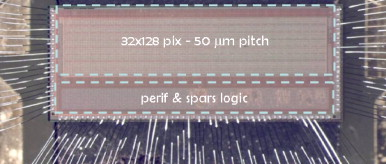
\includegraphics[width=0.45\textwidth]{Apsel.jpg}
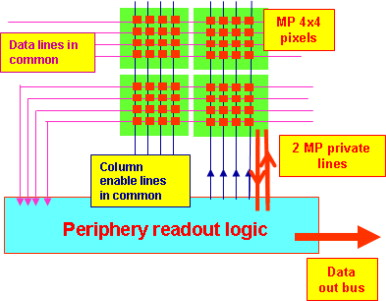
\includegraphics[width=0.45\textwidth]{Apselro.jpg}
\caption{\label{fig:apsel}(left)The Apsel4D chip bonded to the chip carrier. (right)Schematic block diagram of the architecture for MAPS matrix readout.}
\end{figure}

The elementary pixel cell includes a collecting electrode, featuring a buried deep n-type layer, and the full readout chain for signal processing~\cite{Ratti:2006zz}. The processing chain consisted of a charge 
preamplifier with charge to voltage conversion independent of the detector capacitance, a shaping 
stage featuring a 200 or 400~ns peaking time and finally a discriminator used to compare the signal witha chip-wide threshold to provide digital information. 
The design of the front-end minimized the amount of PMOS transistors and related n-wells, which act 
like competitive parasitic electrodes. The fraction of deep n-well area (electrode) over the total n-well 
area was of about 90\%. 



The readout architecture of the APSEL4D pixel, capable of performing on-chip data sparsification, was 
data-driven and permits the use of the tracker information to generate a Level 1 trigger. 
The sparsified readout was implemented thanks to the organisation of 4$\times$4 pixels into a macro 
pixel (MP); each MP had only two private lines for point-to-point connection to the peripheral logic:
one line was used to communicate that the MP has got hits, while the second private line was used to 
freeze the MP until it has been read out.  Common horizontal lines are shared among pixels in the 
same row to bring data from the pixels to the periphery, where the association with the proper 
timestamp is performed before sending the formatted data word to the output bus. The architecture is 
presented in Figure~\ref{fig:apsel}.

The chip has been designed to run with a maximum matrix readout rate of 32 hit pixels/clock cycle and 
a local buffer of maximum 160 hits to minimize the matrix sweep time.
The readout clock, designed to run up to 100~MHz, was operated at 20~MHz in the beam test.
Noise performance were estimated in the laboratory to be of about 75~e (ENC) with 20\% dispersion 
across the matrix; the threshold dispersion over the pixels was estimated be about 60~e.

\section{The Striplets Detector}
\label{sec:Striplets}

The DSSD detector prototype  developed within the SLIM5 project was called ``striplets''. They 
were the baseline option for the Layer0 of the SuperB SVT.
The striplets detector was designed and fabricated at FBK-IRST\footnote{now FBK-CMM: \url{http://cmm.fbk.eu/}}.
The striplets detector was indeed a double-sided strip detector, realised on high-resistivity 
$n-$type bulk. A picture of the striplets detector can be seen in Figure~\ref{fig:striplets}.

\begin{figure}[!htpb]
\centering
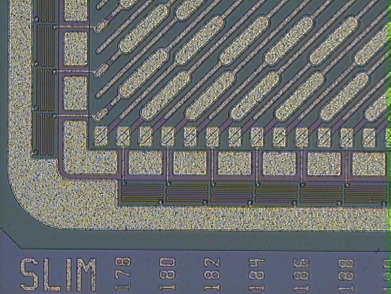
\includegraphics[width=0.5\textwidth]{striplets.jpg}
\caption{\label{fig:striplets} Detail of a corner of the SLIM5 striplet detectors.}
\end{figure}

The striplet geometry was optimized to limit the strip length (18 mm) and the material budget 
(double-sided, 200~$\mu$m thick). The strips were tilted by 45$^{\circ}$ with respect to the 
detector edge, as shown in Figure~\ref{fig:striplets}. The short strip length reduces the average 
occupancy per channel and allows coping with the increased strip-to-backside capacitance, given 
the thin bulk. The strips pitch was 50~$\mu$m on both sides; the detector active area was 
of 27$\times$12.9 mm$^2$. The design allowed a long DSSD with short strips on both sides.
The strips were AC coupled, with integrated capacitors and polisilicon biasing-resistors. 
In order to minimize the dead area along the edges, the resistors are placed outside the guard ring. 
The detector is fully depleted at 10~V bias.

The striplet sensor was read out by the data-driven FSSR2 chip~\cite{Re:2006zw}, 
the second release of the Fermilab Silicon Strip Readout Chip, derived from the one originally designed 
for the silicon pixel detector of the BTeV experiment. The chip is completely data-driven and can be 
readout at up to~70~MHz. The chip features 128 analog channels, with address and time information 
for all hits; the output is purely digital; the chip measures 7.5~mm~$\times$~5~mm and the input pads have an effective pitch of 50~$\mu$m. A picture of the FSSR2 chip is shown in Figure~\ref{fig:fssr2}


\begin{figure}[!htpb]
\centering
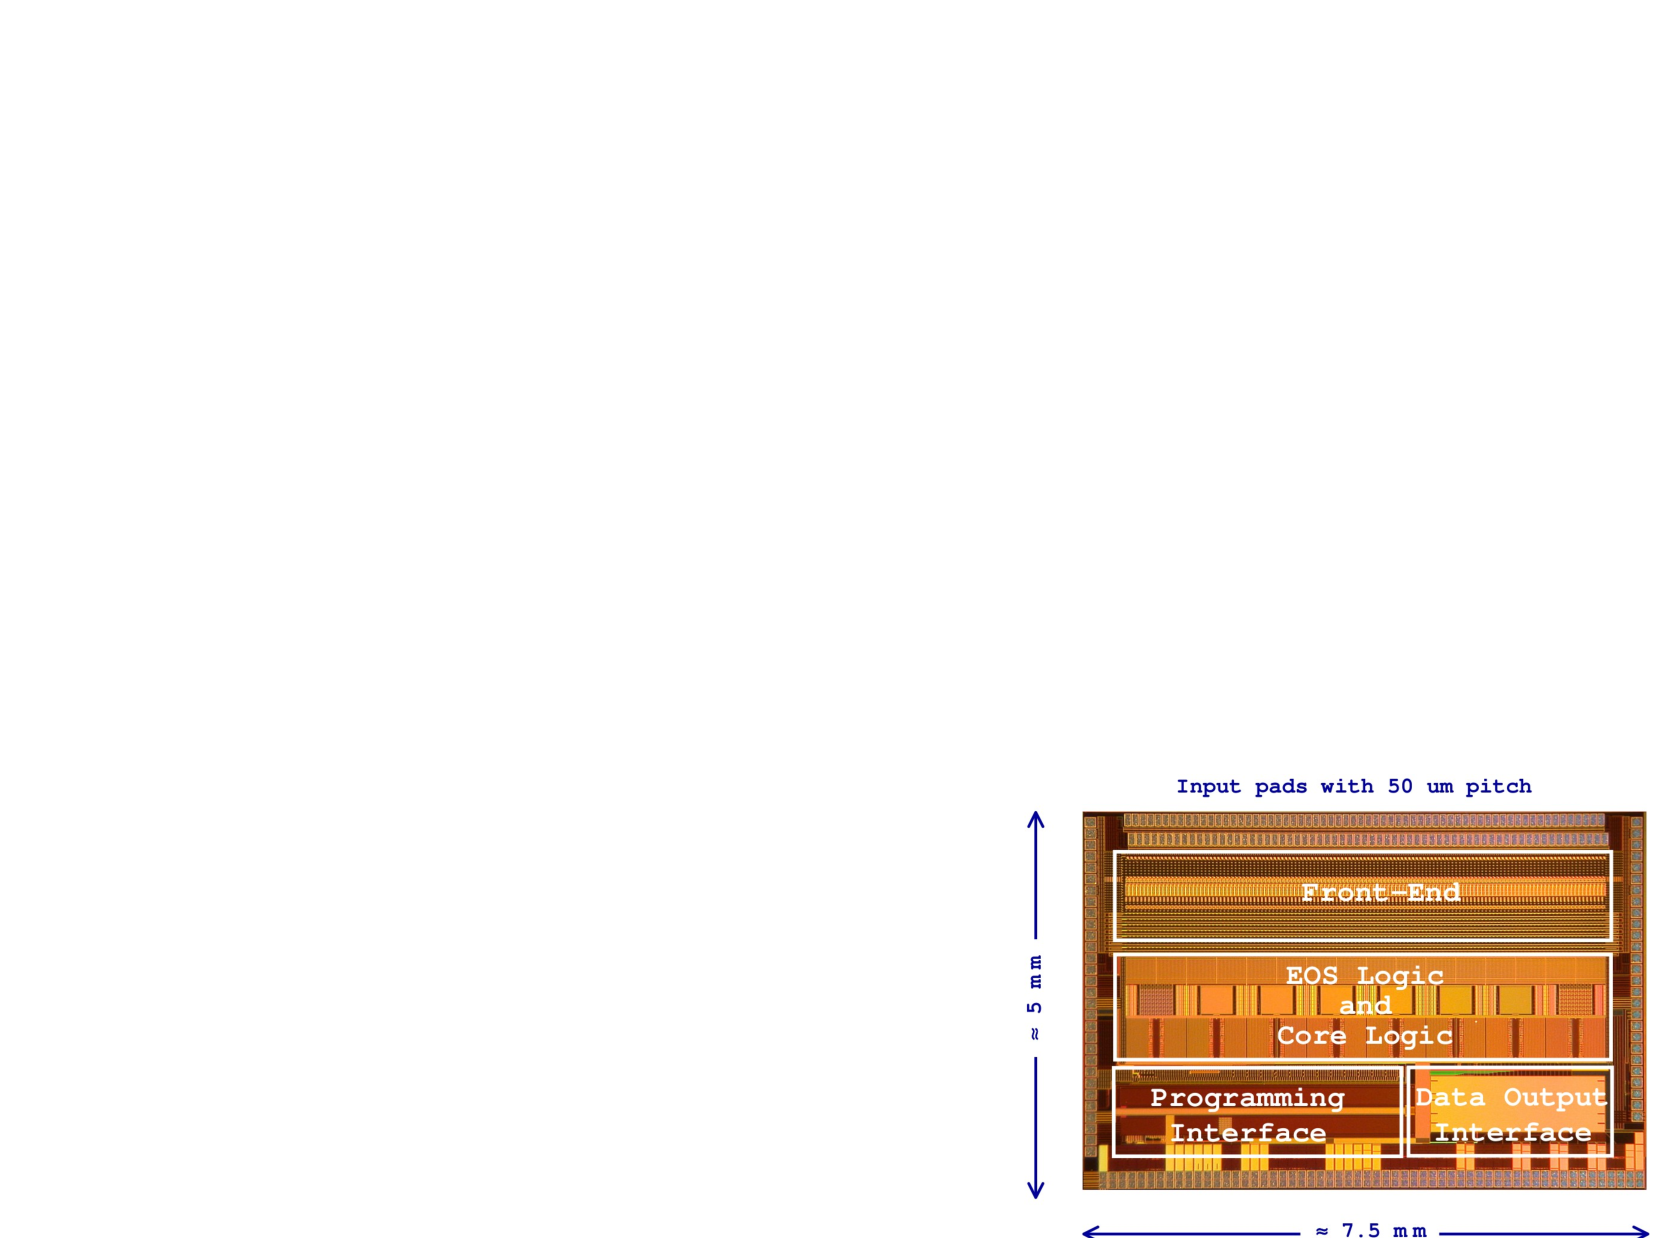
\includegraphics[width=0.5\textwidth]{fssr2.pdf}
\caption{\label{fig:fssr2}Annotated picture of the FSSR2 chip with input pads at the top. (Adapted from~\cite{Re:2006zw})}
\end{figure}


FSSR2 chip offers 8 programmable thresholds, with the first one acting as hit/no hit discriminator
({\it zero suppression} mode), 
so each hit has a 3-bits adc information. The design was optimised for positive signals; 
here for the first time it was used to read out negative signals too (ohmic side of the striplets). 
Due to the limited dynamic range for $n$-side just a hit/no hit information for negative signals was 
extracted.

In Figure~\ref{fig:assembled_striplets} a striplet detector module is shown.

\begin{figure}[!htpb]
\centering
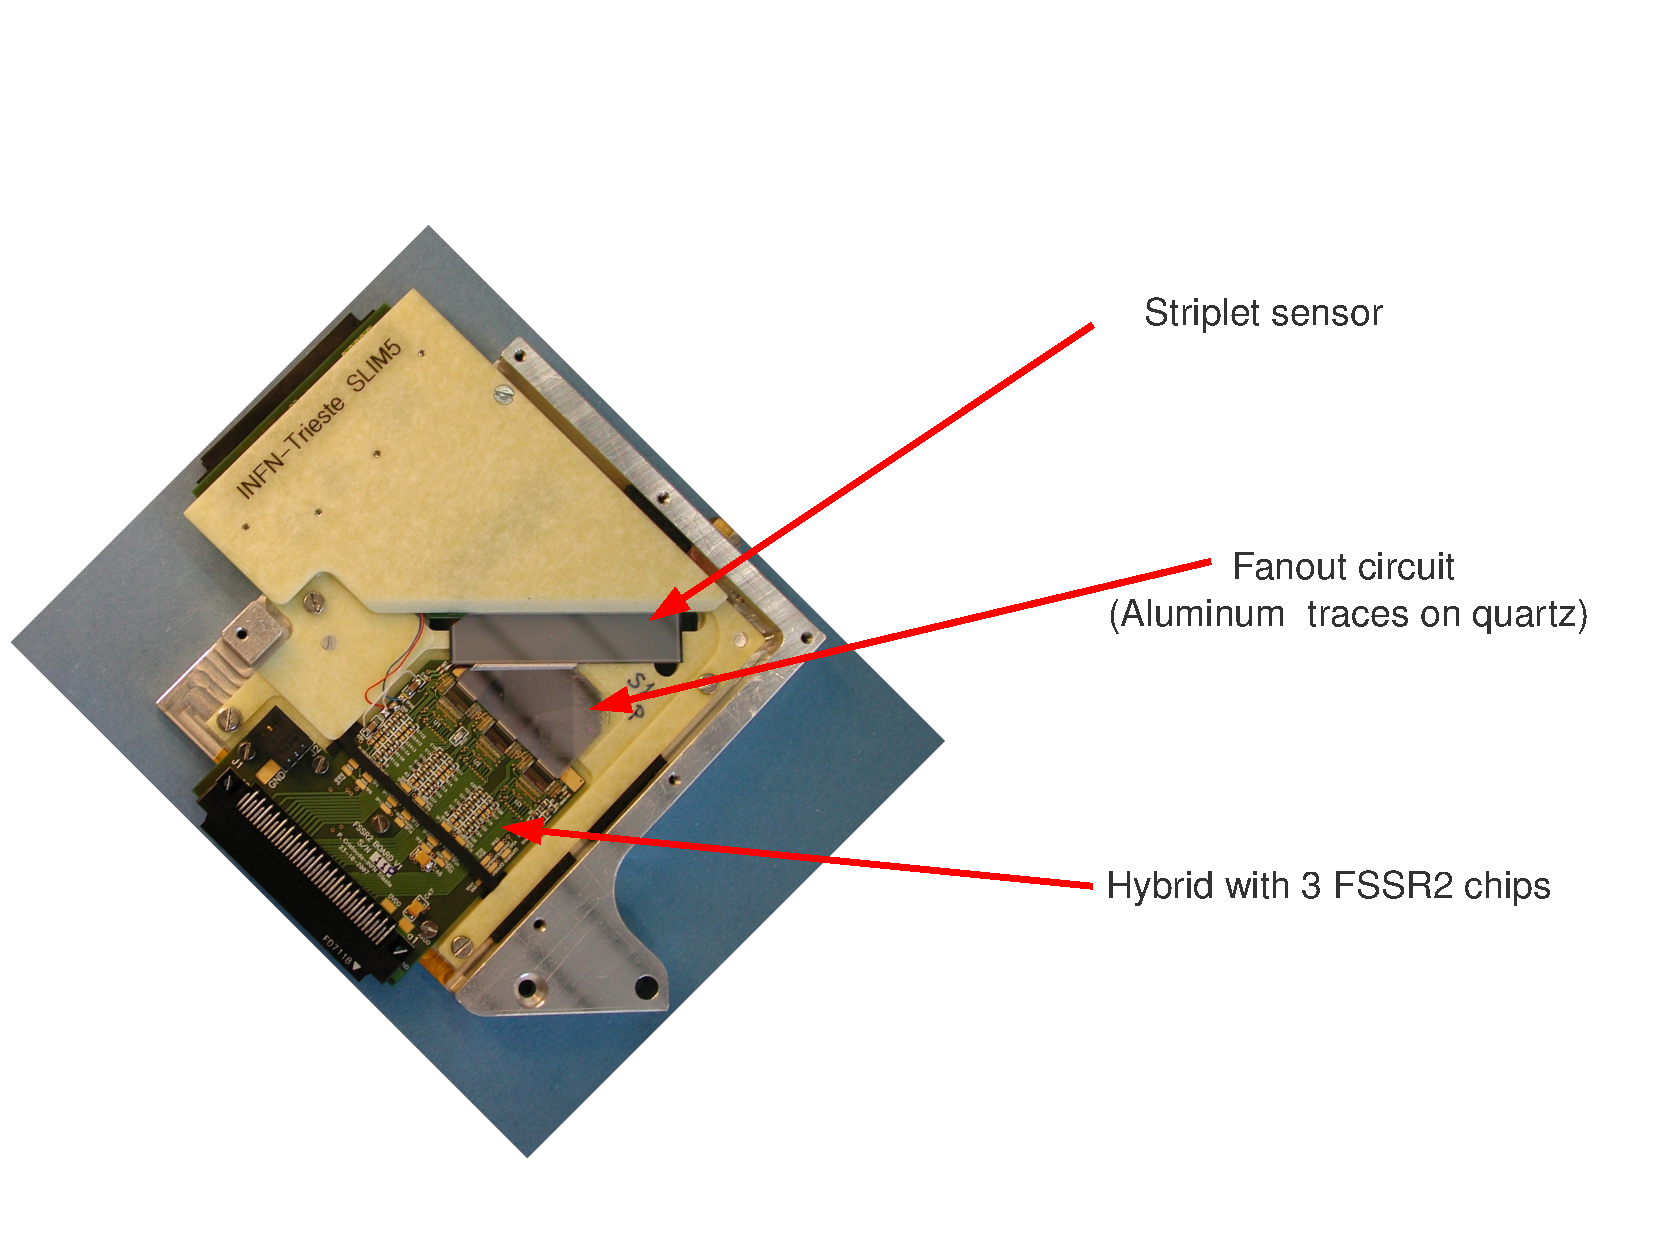
\includegraphics[width=0.95\textwidth]{assembeld_striplets.pdf}
\caption{\label{fig:assembled_striplets}Annotated picture of an assembled striplet module. The 
sensor, the fanout circuit and the readout card, hosting 3 FSSR2 chips, are visible.}
\end{figure}

One striplet sensor was read out by 3 FSSR2 chips per side, for a total of 384 wirebonded channels 
on each side. 

\section{Performance of SLIM5 Detectors}
\label{sec:SLIM5Results}
To fully test the detector prototypes a demonstrator was built~\cite{BETTARINI2010942} and put  on 
beam at the T9 facility of the CERN PS in September 2008.

\subsection{The experimental set-up}

At T9 facility of the CERN PS protons of 12~GeV/c, with spills of 400 ms and typically from 10$^4$ to
 10$^6$ particles/spill, where impinging on the demonstrator, which was set-up as shown if 
 Figure~\ref{fig:slim5_tb}.

\begin{figure}[!htpb]
\centering
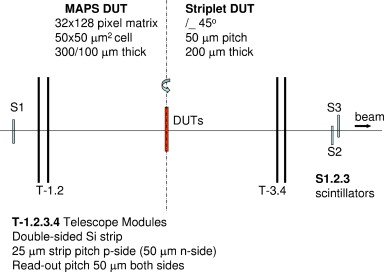
\includegraphics[width=0.45\textwidth]{slim5_tb.jpg}
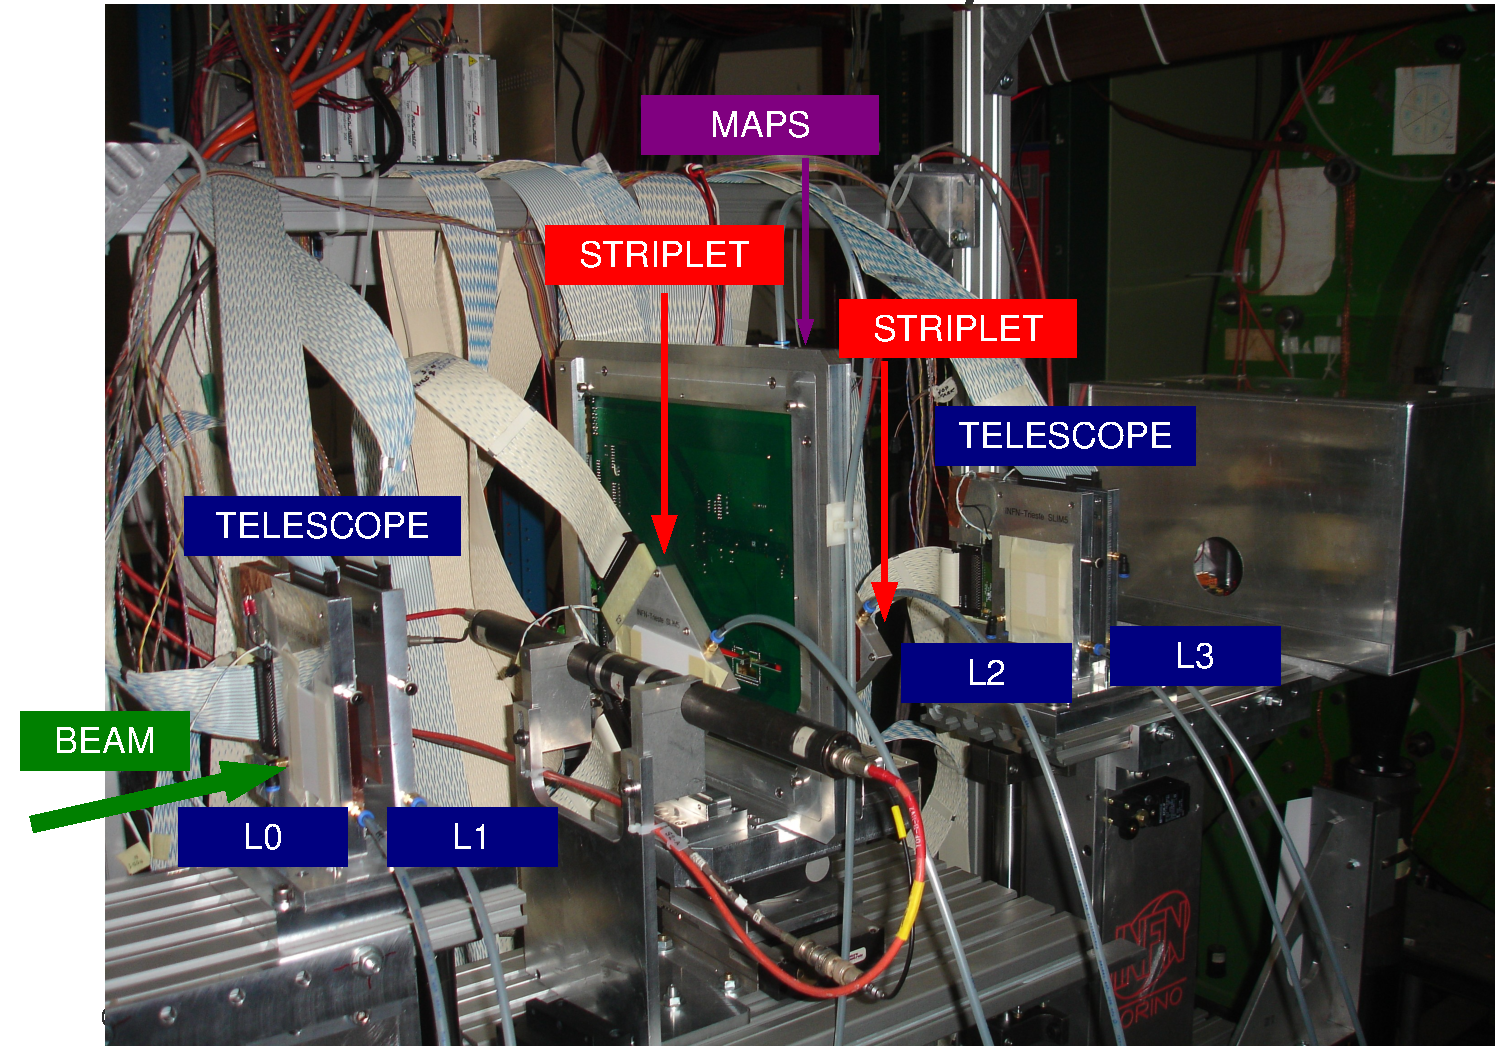
\includegraphics[width=0.45\textwidth]{tbpic.pdf}
\caption{\label{fig:slim5_tb}(left)The SLIM5 Beam Test Setup. (right)Picture of the SLIM5 demonstrator at the T9 facility of the CERN PS in September 2008. The telescope, 2 striplets modules and 
one Apseld4D are visible.}
\end{figure}



For the reference telescope, we used four 2~$\times$~2~cm$^{2}$ DSSDs where used; 
the strips where AC-coupled, with 25~(50)~$\mu$m pitch on $p-(n-)$side. The readout pitch 
was the same (50~$\mu$m) for both sides, as the telescope modules too were readout by 
the FSSR2 chip. One pair was positioned upstream and the other downstream of the devices 
under test (DUTs). The scintillators ($S1$, $S2$ and $S3$) were used for trigger studies.

\subsection{Apsel4D Results}
Two Apsel4Ds were studied, one having with nominal thickness (300~$\mu$m) and the other 
thinned down to 100~$\mu$m only. The maximum efficiency was observed for the 
thinned chip; at the lowest threshold (400~e, about 40\% of a MIP signal) it reached~92\%, which roughly corresponds to 
the Apseld4D fill factor. 
Efficiency vs threshold results for Apsel4D are shown in~Figure~\ref{fig:maps_eff}

\begin{figure}[!htpb]
\centering
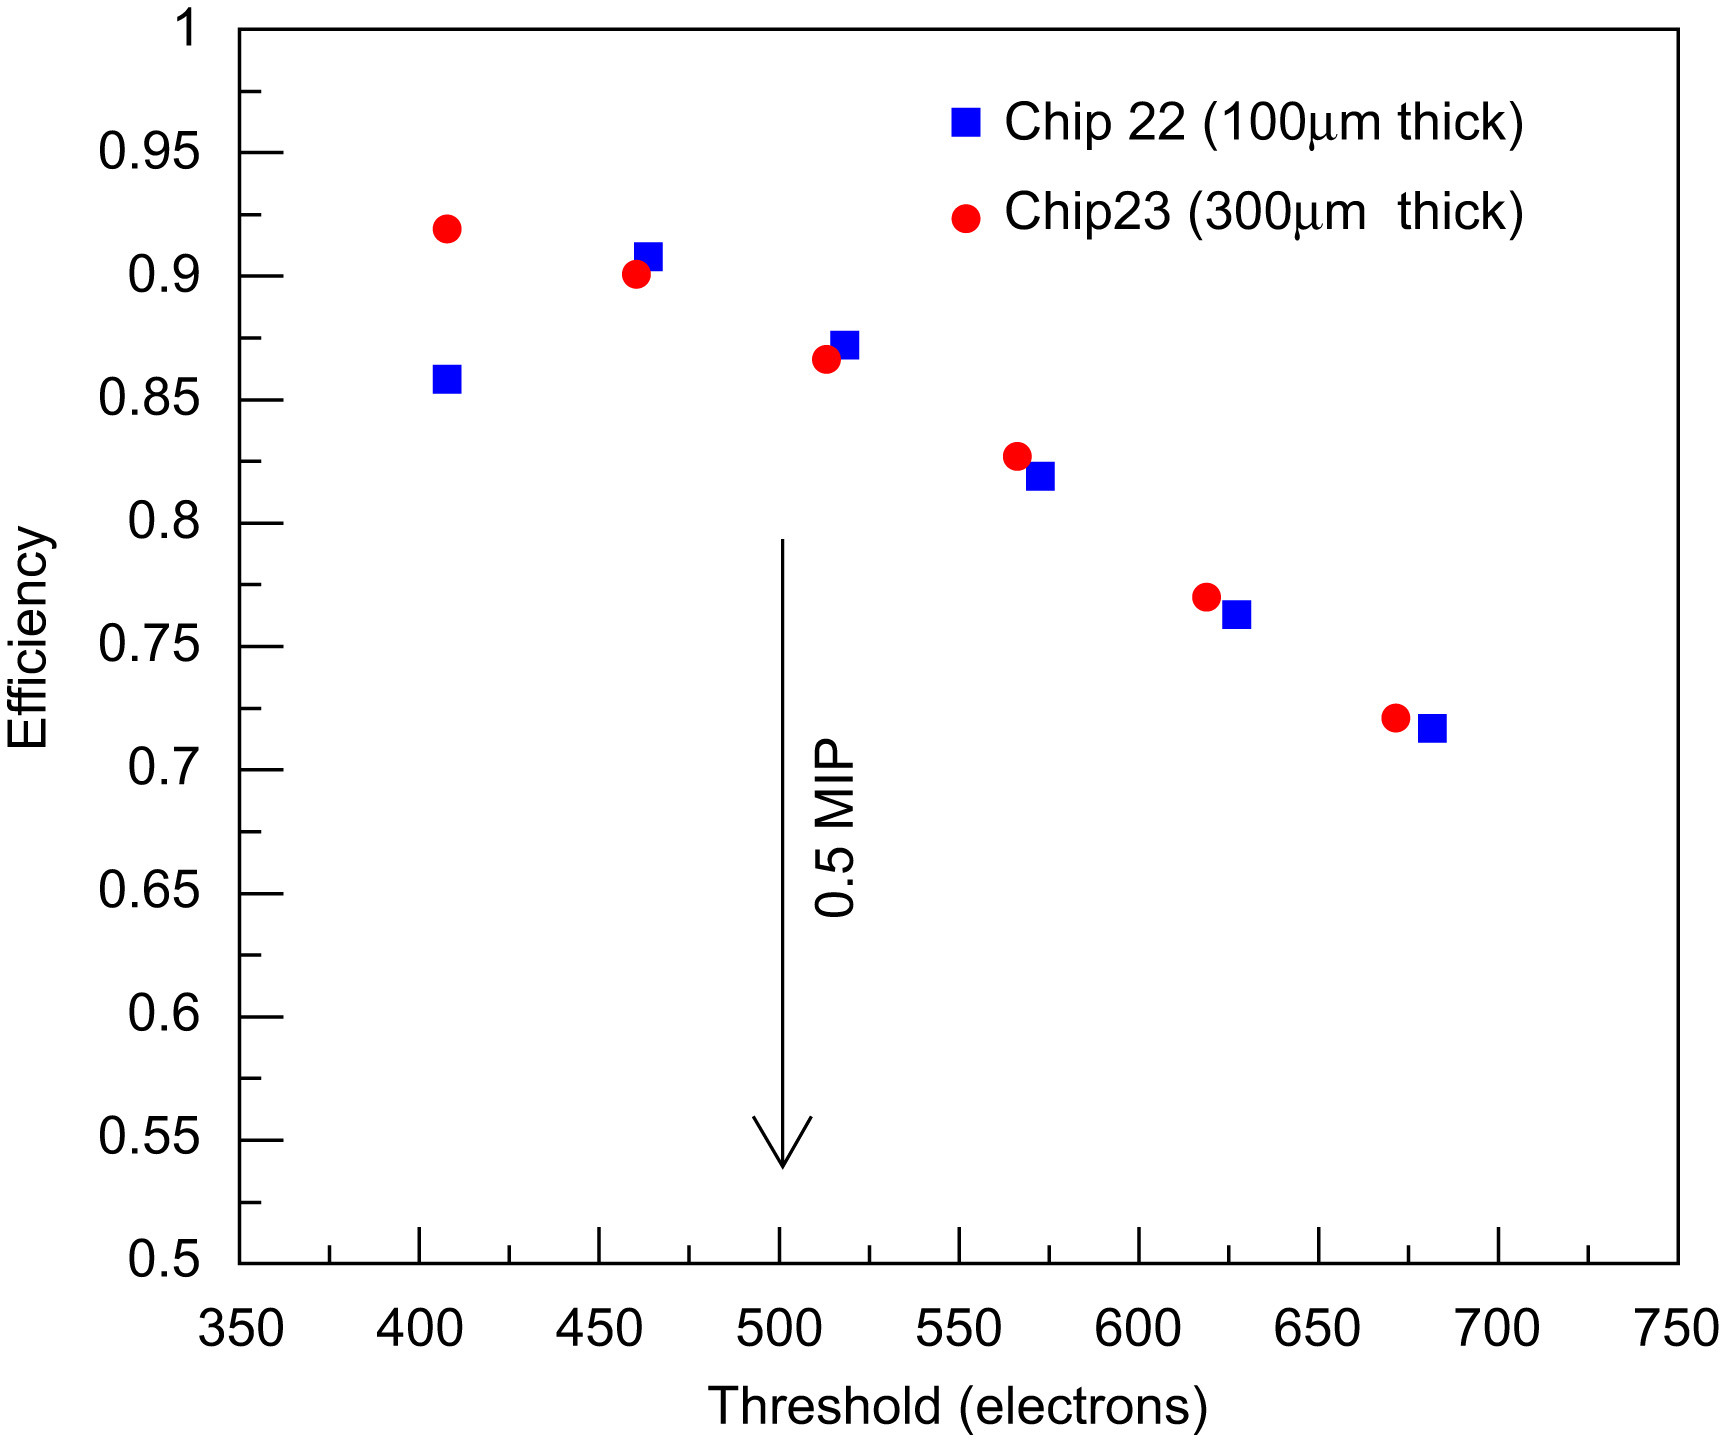
\includegraphics[width=0.45\textwidth]{maps_eff.jpg}
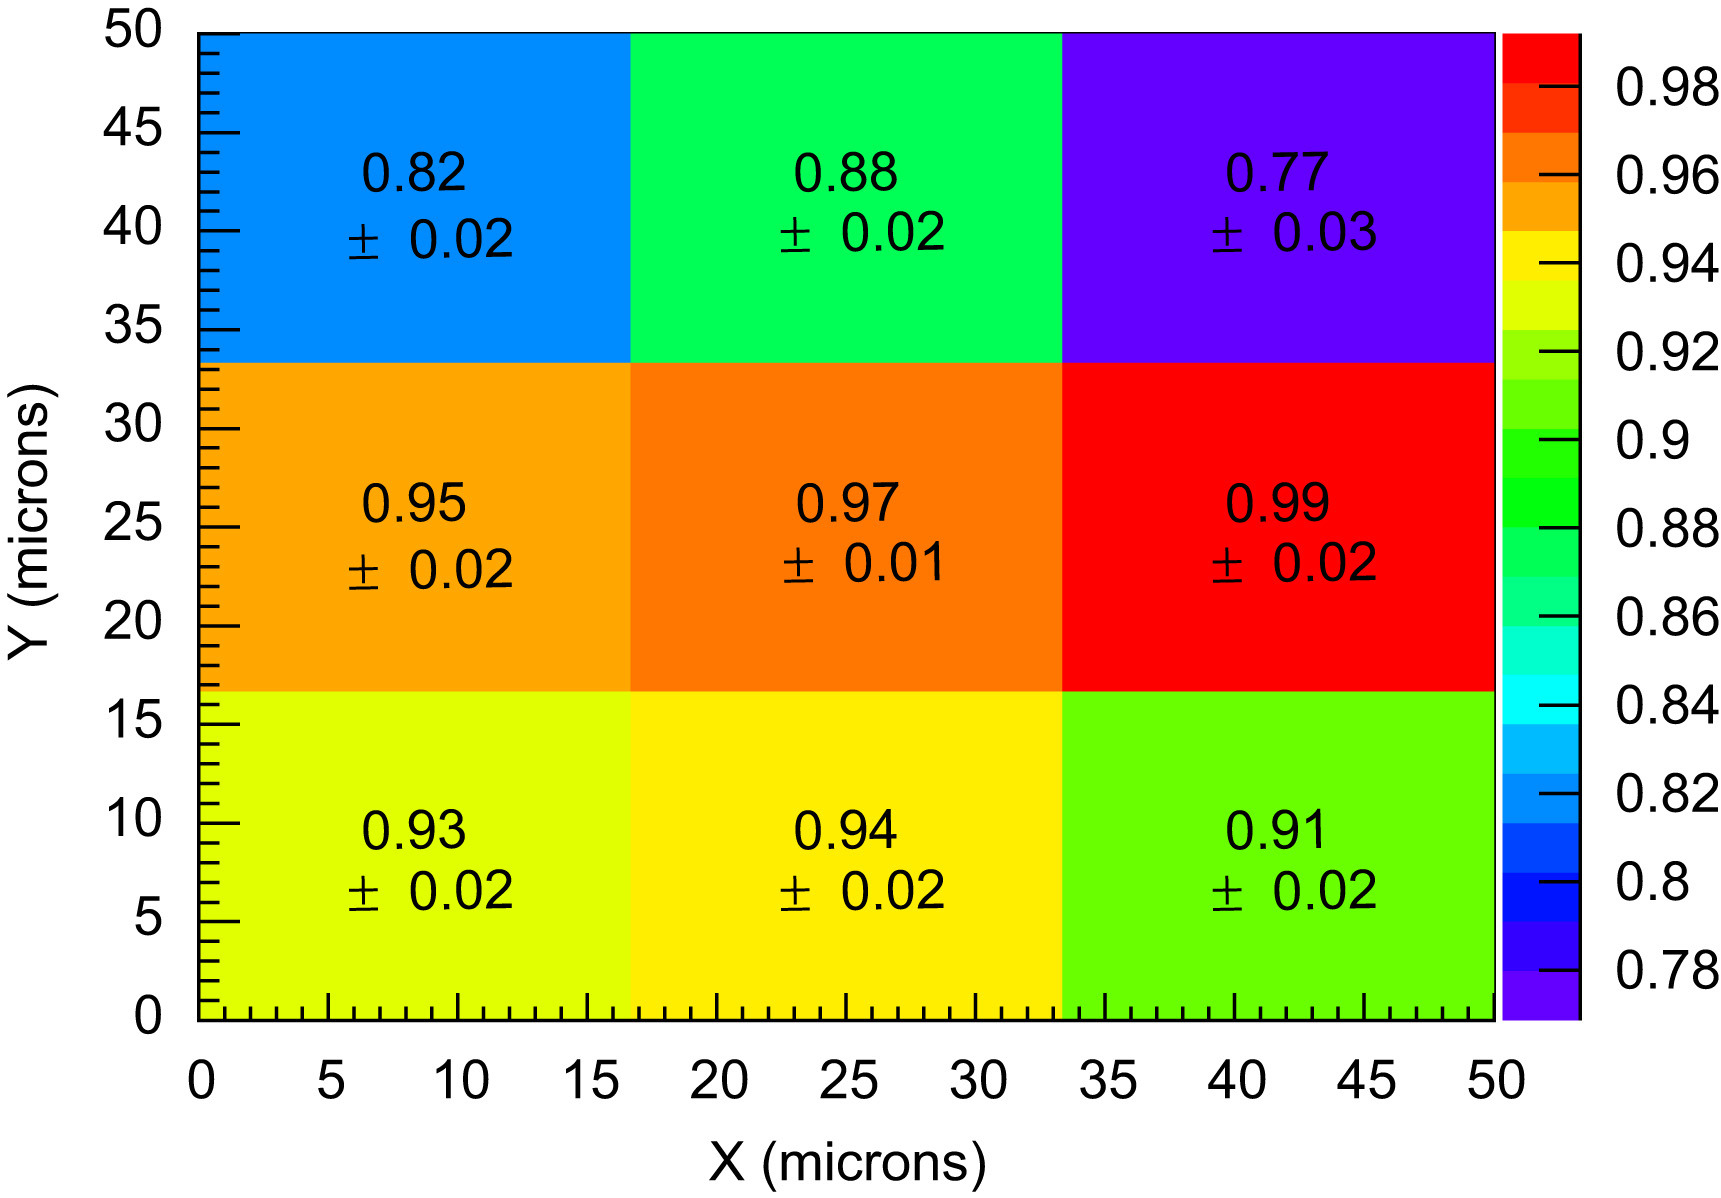
\includegraphics[width=0.45\textwidth]{maps_res.jpg}
\caption{\label{fig:maps_eff}(left)Efficiency results for two MAPS detectors, taken from a single threshold 
scan. The statistical uncertainty on each point is smaller than the size of the plotting symbol. The point 
of low efficiency at the lowest threshold was probably due to temperature fluctuations during the 
measurements.(right) MAPS hit efficiencies measured as a function of position within the pixel. The picture, which is not to scale, represents a single pixel divided into nine sub-cells. The values are the efficiencies obtained in each sub-cell after taking into account track migration among cells. The uncertainties include the statistical uncertainty plus a systematic contribution coming from the track migration.}
\end{figure}
The efficiency within the Apsel4D pixel cell was performed; given the tracking resolution 
of about~7~$\mu$m the Apsel4D pixel cell was divided in a 3~$\times$~3 matrix. The results 
are reported in~Figure~\ref{fig:maps_eff}


One observes a significant variation of sensibility within the pixel area, as expected. In particular, the central region is seen to be virtually 100\% efficient, while the upper part of the pixel, especially the upper right-hand sub-cell, shows lower efficiency due to the presence of competitive n-wells.

The measured intrinsic hit resolution was about 14~$\mu$m for the X-coordinate and slightly better 
for the Y-coordinate: a modest improvement with respect to the single pixel hit resolution of 
50~$\mu\,/\,\sqrt{12}$=14.4~$\mu$m, mainly due 
to the absence of analog information and to the modest fraction of clusters of two or more pixels.

\subsection{Striplets Results}

The results from the testbeam of a striplet module are outlined in this Section; in the following one
a discussion on the impact of threshold on residuals will be presented.

We have evaluated the input noise charge by measuring the fraction of hits over
 threshold as a
function of the input charge at a given discriminator threshold.
The results of the calibrations are summarised in Table~\ref{tab:FSSR2Calib}.


\begin{table}[hbt]
\begin{center}
\caption{Calibration results for the striplet detectors.
\label{tab:FSSR2Calib}}
\vspace{\baselineskip}
\begin{tabular}{|c|c|c|}
\hline

Side & $p$  & $n$ \\

\hline
Noise (e)& 630       & 1020   \\
S/N      & 25        & 16         \\
Gain (mV/fC)& 96     & 67         \\
Threshold (e) & 4400 & 6300 \\
Thr.Dis. (e)& 880       & 780\\ \hline
\end{tabular}
\end{center}
\end{table}

Cluster of strips were created by grouping neighbouring strips that have fired. The charge pulse height 
distribution of clusters are shown in Figure~\ref{fig:clu_ph_striplets}.

\begin{figure}[!htpb]
\centering
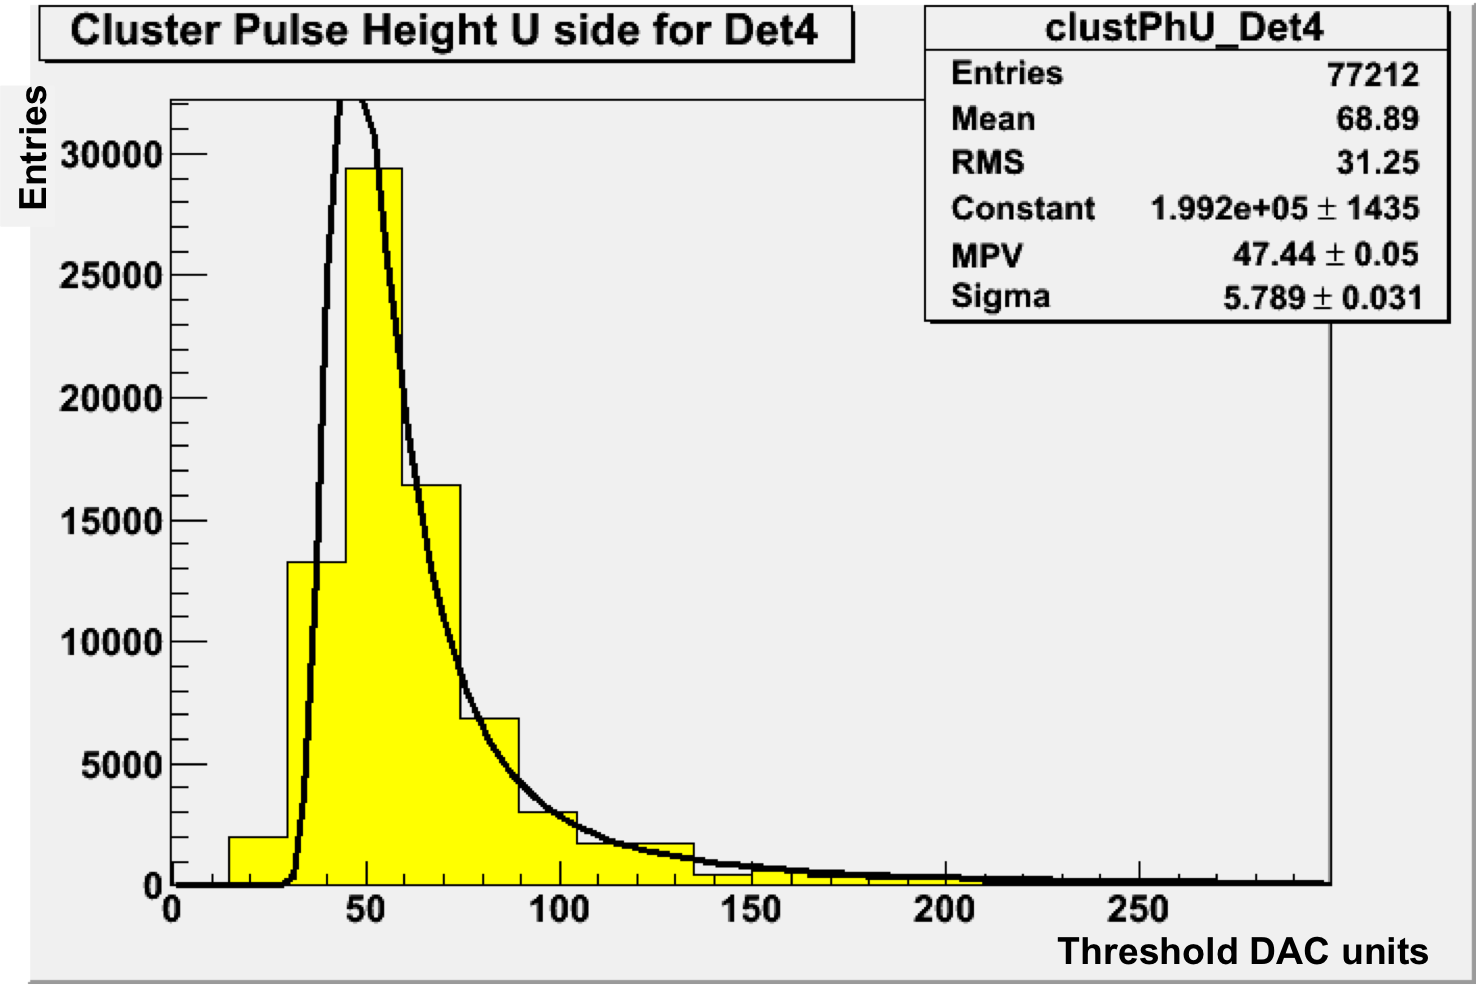
\includegraphics[width=0.45\textwidth]{p_side_striplets.png}
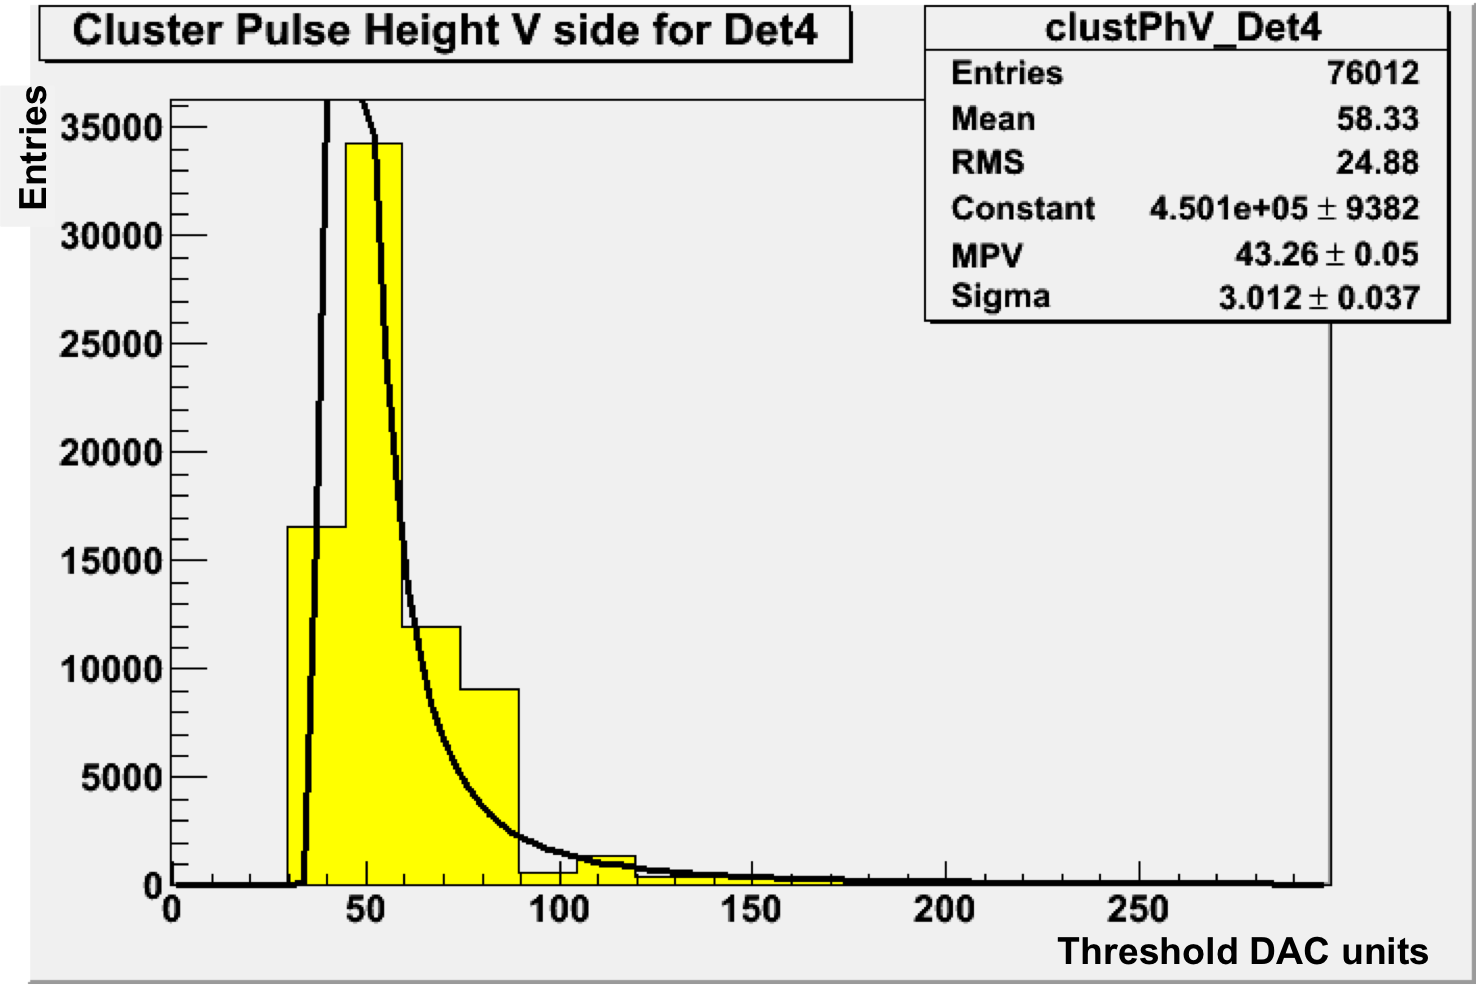
\includegraphics[width=0.45\textwidth]{n_side_striplets.png}
\caption{\label{fig:clu_ph_striplets}Cluster pulse height distribution for a striplet module. (left) $p-$ side; 
(right) $n-$side. Data is fitted with a Landau function.}
\end{figure}

The fitted MPV was found to be well compatible with the expected  value for a MIP in 200~$\mu$m 
thick silicon detector. The region above 100 threshold DAC for the $n-$side was severely impacted 
by the limited dynamical range of the ADC, as it can be seen in Figure~\ref{fig:clu_ph_striplets}.

The hit-efficiency was of above 98\% for both the $p-$ and the $n-$side. A detailed analysis 
of the hit-efficiency as a function of the position along the detector is shown in 
Figure~\ref{fig:striplets_eff}.


\begin{figure}[!htpb]
\centering
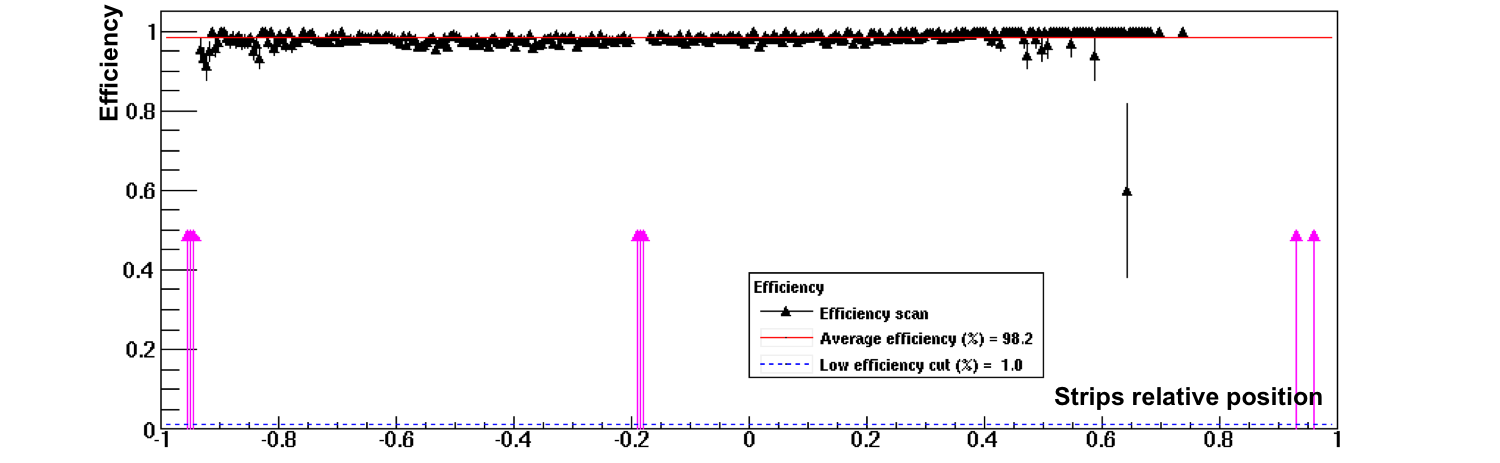
\includegraphics[width=0.95\textwidth]{striplets_eff.png}
\caption{\label{fig:striplets_eff}Efficiency of a striplet module as a function of the track impact position. 
Dead strips where removed from the analysis by selecting strips with efficiency greater than 1.0\%; 
their position is marked by magenta arrows.}
\end{figure}

As it can be seen efficiency was quite uniform
over the entire sensor. Strips with efficiency below 1\% where declared as dead and removed from the 
analysis. An electrical analysis after the testbeam confirmed that  the dead strips 
were indeed disconnected/malfunctioning channels. 

The spatial resolution performance of the striplets will be discussed in detail in the next Section.

\section{Discussion of the Striplets Spatial Resolution}
\label{sec:striplets_res}

In this Section the spatial resolution of the striplets will be discussed in detail. 

\subsection{Residuals and Spatial Resolution}

The spatial resolution performance of position sensitive silicon detectors depends on various factors; 
some of them are related to the physics processes of charge creation and transport, others to 
the detector characteristics. 
Among the former there is the statistical fluctuation 
of the energy loss 
 and the diffusion of the charge carriers produced by the MIP: the carriers created by a traversing MIP 
 spreads  due to diffusion according to $\sigma = \sqrt{2Dt}$ where $D$ is the diffusion constant and 
 $t$ is the time the carriers travel to reach the collecting electrode; typical values of the diffusion 
 spread $\sigma$ are of few $\mu$m for detector thicknesses of 100-200~$\mu$m when the  
  carriers velocities are saturated.
Factors that influence the spatial resolution that are related to the  detector characteristics are the 
analog or digital readout, the detector pitch and the signal-to-noise ratio.

Spatial resolution is usually estimated by taking the RMS of the residuals distribution. Residuals are 
defined as the difference between the position of the DUT hit associated to a track and 
the extrapolated position on the DUT plane of the track itself. 
The width of the residuals distribution depends on many factors: the intrinsic resolution of the 
DUT (about the detector pitch divided by $\sqrt{12}$ - the so-called {\it digital resolution}~\cite{TURCHETTA}), the pointing resolution of the tracking system 
(about the intrinsic resolution of each telescope plane divided by the square root of the number of 
telescope planes) and the RMS deviation due to MS,

\begin{equation}
\sigma_{res}=\sigma_{DUT}\oplus\sigma_{trk}\oplus\sigma_{MS}
\label{eq:res}
\end{equation}

If the contribution of tracking and MS to the residuals is negligible with respect to the DUT 
one, then the DUT elementary cell, strip or pixel, can be resolved (examples can be found 
in~\ref{sec:radhardpixels}); if not, then the residuals distribution 
is usually well described by a Gaussian distribution. 

Charge sharing between neighbouring strips (or pixels) allow the formation of clusters with 2 
or more. Focusing on strips, when more than 1 strip fires it is important to assign to the 
multi-strips clusters the positions that give as a result the smallest possible residuals distribution, 
hence, the ultimate spatial resolution for the detector. 


In~\cite{TURCHETTA} an excellent and complete discussion on the best algorithms to find 
the position of particle hits is given; the influence of detector parameters (thickness, pitch, 
floating strips, etc.) and of the track angle are investigated.
The best algorithm for clusters of 2 strips is the so-called $\eta$ position-finding algorithm (PFA), 
where:

\begin{equation}
\eta=\dfrac{S_R}{S_R+S_L}
\label{eq:eta}
\end{equation} 
where $S_{R(L)}$ is the signal amplitude of the right (left) strip in the cluster.
Using the $\eta$  PFA the cluster position $x_{\eta}$ is defined as:
 \begin{equation}
\dfrac{x_{\eta}}{P}=f(\eta)+\dfrac{x_L}{P}
\label{eq:xeta}
\end{equation} 

where $P$ is the detector pitch, $x_L$ is the center position of the left strip in the cluster and 
$f(\eta)$ is a function that can be estimated directly on data:

\begin{equation}
f(\eta)=\dfrac{\int_0^\eta \dfrac{{\rm d}N}{{\rm d}\eta'}{\rm d}\eta'}{\int_0^1 \dfrac{{\rm d}N}{{\rm d}\eta'}{\rm d}\eta'}
\end{equation}

under the assumption that the distribution of the number of tracks $N$ is uniform between 
the left and right strip.

The uncertainty  on the position identified using the  $\eta$ PFA $\sigma_{\eta}$, hence the detector spatial 
resolution, is about the detector pitch $P$ 
divided by the signal (S) over noise (N) ratio:

\begin{equation}
\dfrac{\sigma_{\eta}}{P}\sim\dfrac{N}{S}
\label{eq:etanoise}
\end{equation}

The $\eta$ algorithm is the optimal one for tracks at normal incidence or impinging at small angles. 
Despite it was used for the analysis of striplets data the width of residuals was much 
larger than expectations, about 16~$\mu$m with respect to $\sim$14~$\mu$m that is the 
expected value  for hits formed by just 1 strip. The reason for this poor resolution 
was investigated and the results are discussed in what follows.

\subsection{Striplets Residuals and the Effect of Thresholds}

In Figure~\ref{fig:res_pside} the residuals distribution for hits registered on the $p-$side of a striplet 
module. The width of the fitted Gaussian is about 16~$\mu$m.

\begin{figure}[!htpb]
\centering
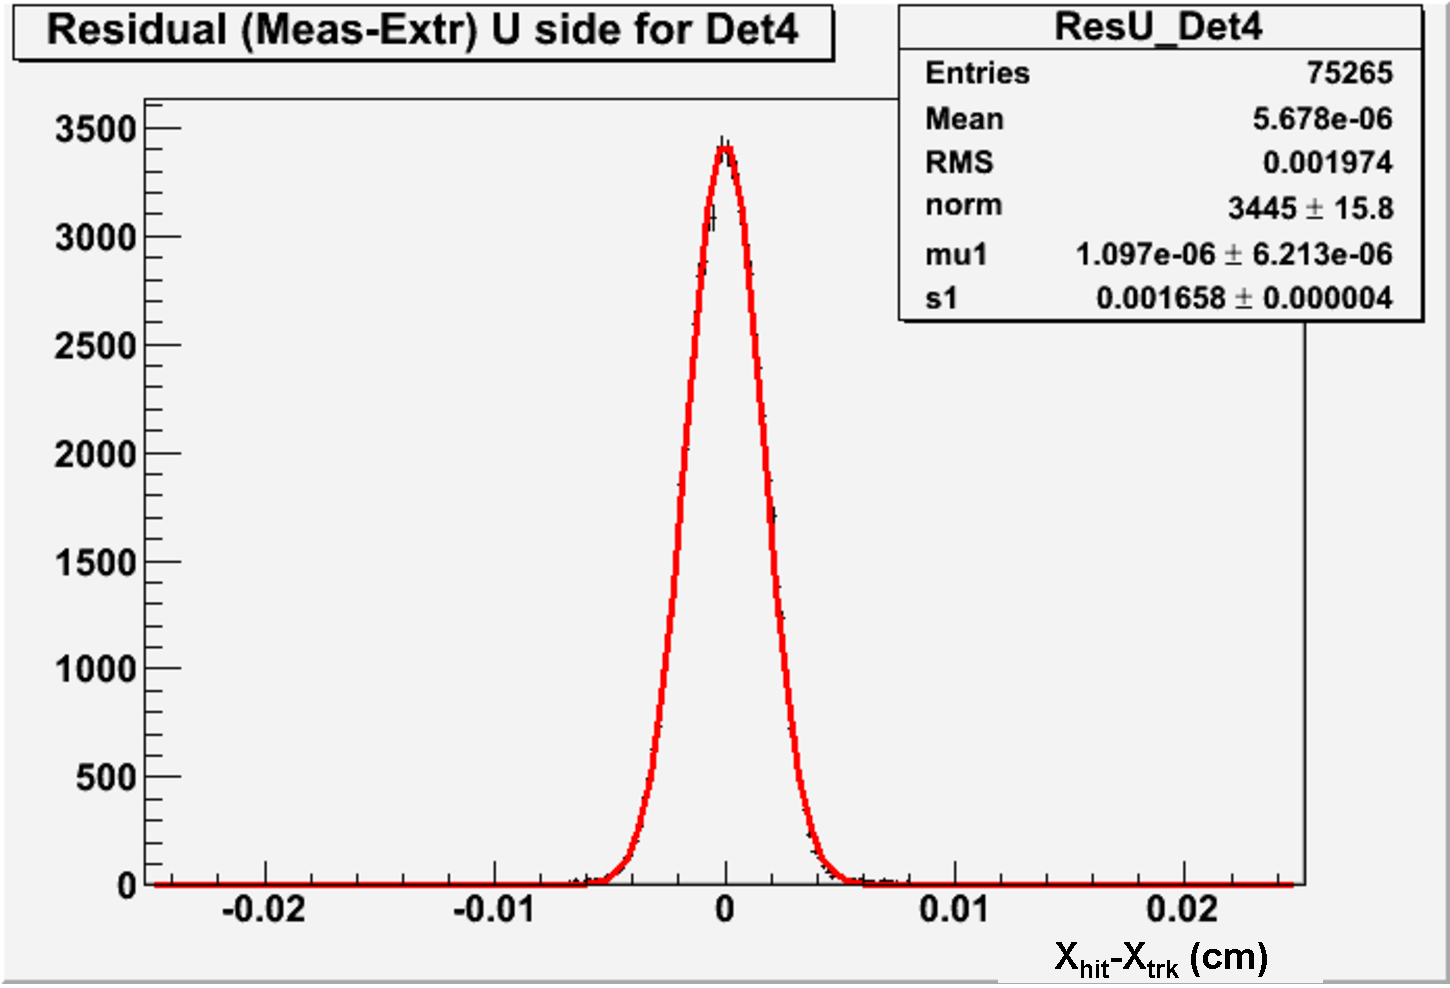
\includegraphics[width=0.5\textwidth]{res_pisde.pdf}
\caption{\label{fig:res_pside}Residuals distribution for hits registered on the $p-$side of a 
striplets module. Points are data, the red line is the result of a Gaussian fit to the distribution.}
\end{figure}

More than 82\% of the analysed clusters contained just 1 strip when particles where impinging 
at normal incidence; 16\% of the total had 2 strips. Hence the expected residuals width when all 
clusters are analysed together should have been slightly smaller than 
$50/\sqrt{12}\approx 14.4\, \mu$m. 

The reason for the poor performance was found to be related to the high hit/no hit threshold set 
on the FSSR2 chip. In case of asymmetric charge sharing between two strips one of the two 
can have a signal that is below threshold, hence a true cluster of 2 strips is reconstructed as a single 
strip. In this case the cluster position is assigned to the center of the only strip whose signal is 
above threshold, so, on average, the error made in position assignment is about half of the pitch, 
{\it i.e.} 25~$\mu$m.

To confirm the hypothesis clusters with charge about or less than
 a third (6600~e) the one expected for a MIP where 
studied; the residuals distribution for these clusters is show in 
Figure~\ref{fig:annotated_res_pside_1stPHbin}.Two peaks around $P/2\approx25\,\mu$m are clearly visible: they correspond to the aforementioned true 2 strips clusters reconstructed as 1 strip only 
hit.


\begin{figure}
\centering
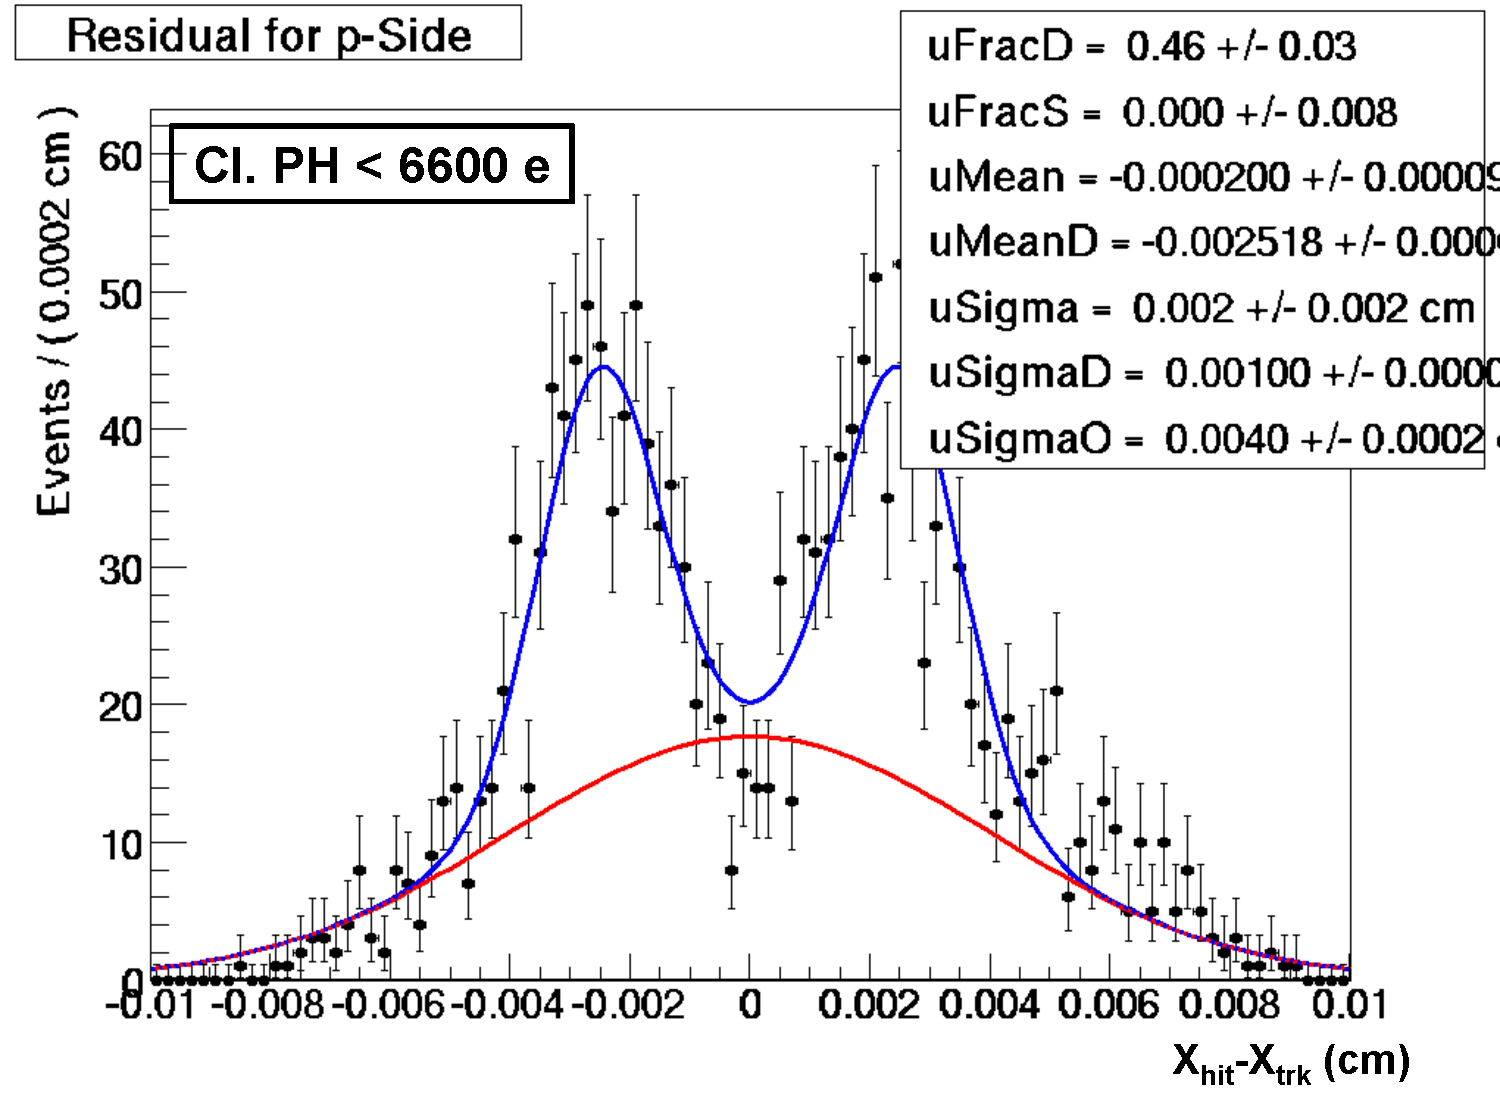
\includegraphics[width=0.5\textwidth]{annotated_res_pside_1stPHbin.pdf}
\caption{\label{fig:annotated_res_pside_1stPHbin}Residuals distribution for hits registered on the $p-$side of a 
striplets module when only clusters with $\le$6600~e charge are considered. Data are represented as points with error bars. The fit function (blue solid line) is given in Equation~\ref{eq:res_pdf}; the red solid line 
is the outlier Gaussian contribution.}
\end{figure}

The residuals distribution was then fitted with a function containing three components: a core 
Gaussian, to model correctly reconstructed clusters; a double guassian, with mean fixed at 
$\pm 25\, \mu$m, to model the mis-reconstructed 2 strips clusters; and finally an outlier Gaussian, 
with mean fixed at 0~$\mu$m, to take into account spurious hits. 
The probability density function (PDF) as a function of the residual value $x$ was:

\begin{equation}
f(x)=f_S S(x)+(1-f_S)\Big[  f_DD(x)+(1-f_D)O(x) \Big]
\label{eq:res_pdf}
\end{equation}

where S, D and O are the core, double and outlier Gaussian, respectively, and $f_{S,D}$ are 
weights constrained between 0 and 1. 

The distribution of residuals of all clusters are shown in Figure~\ref{fig:striplets_residuals}. 

\begin{figure}
\centering
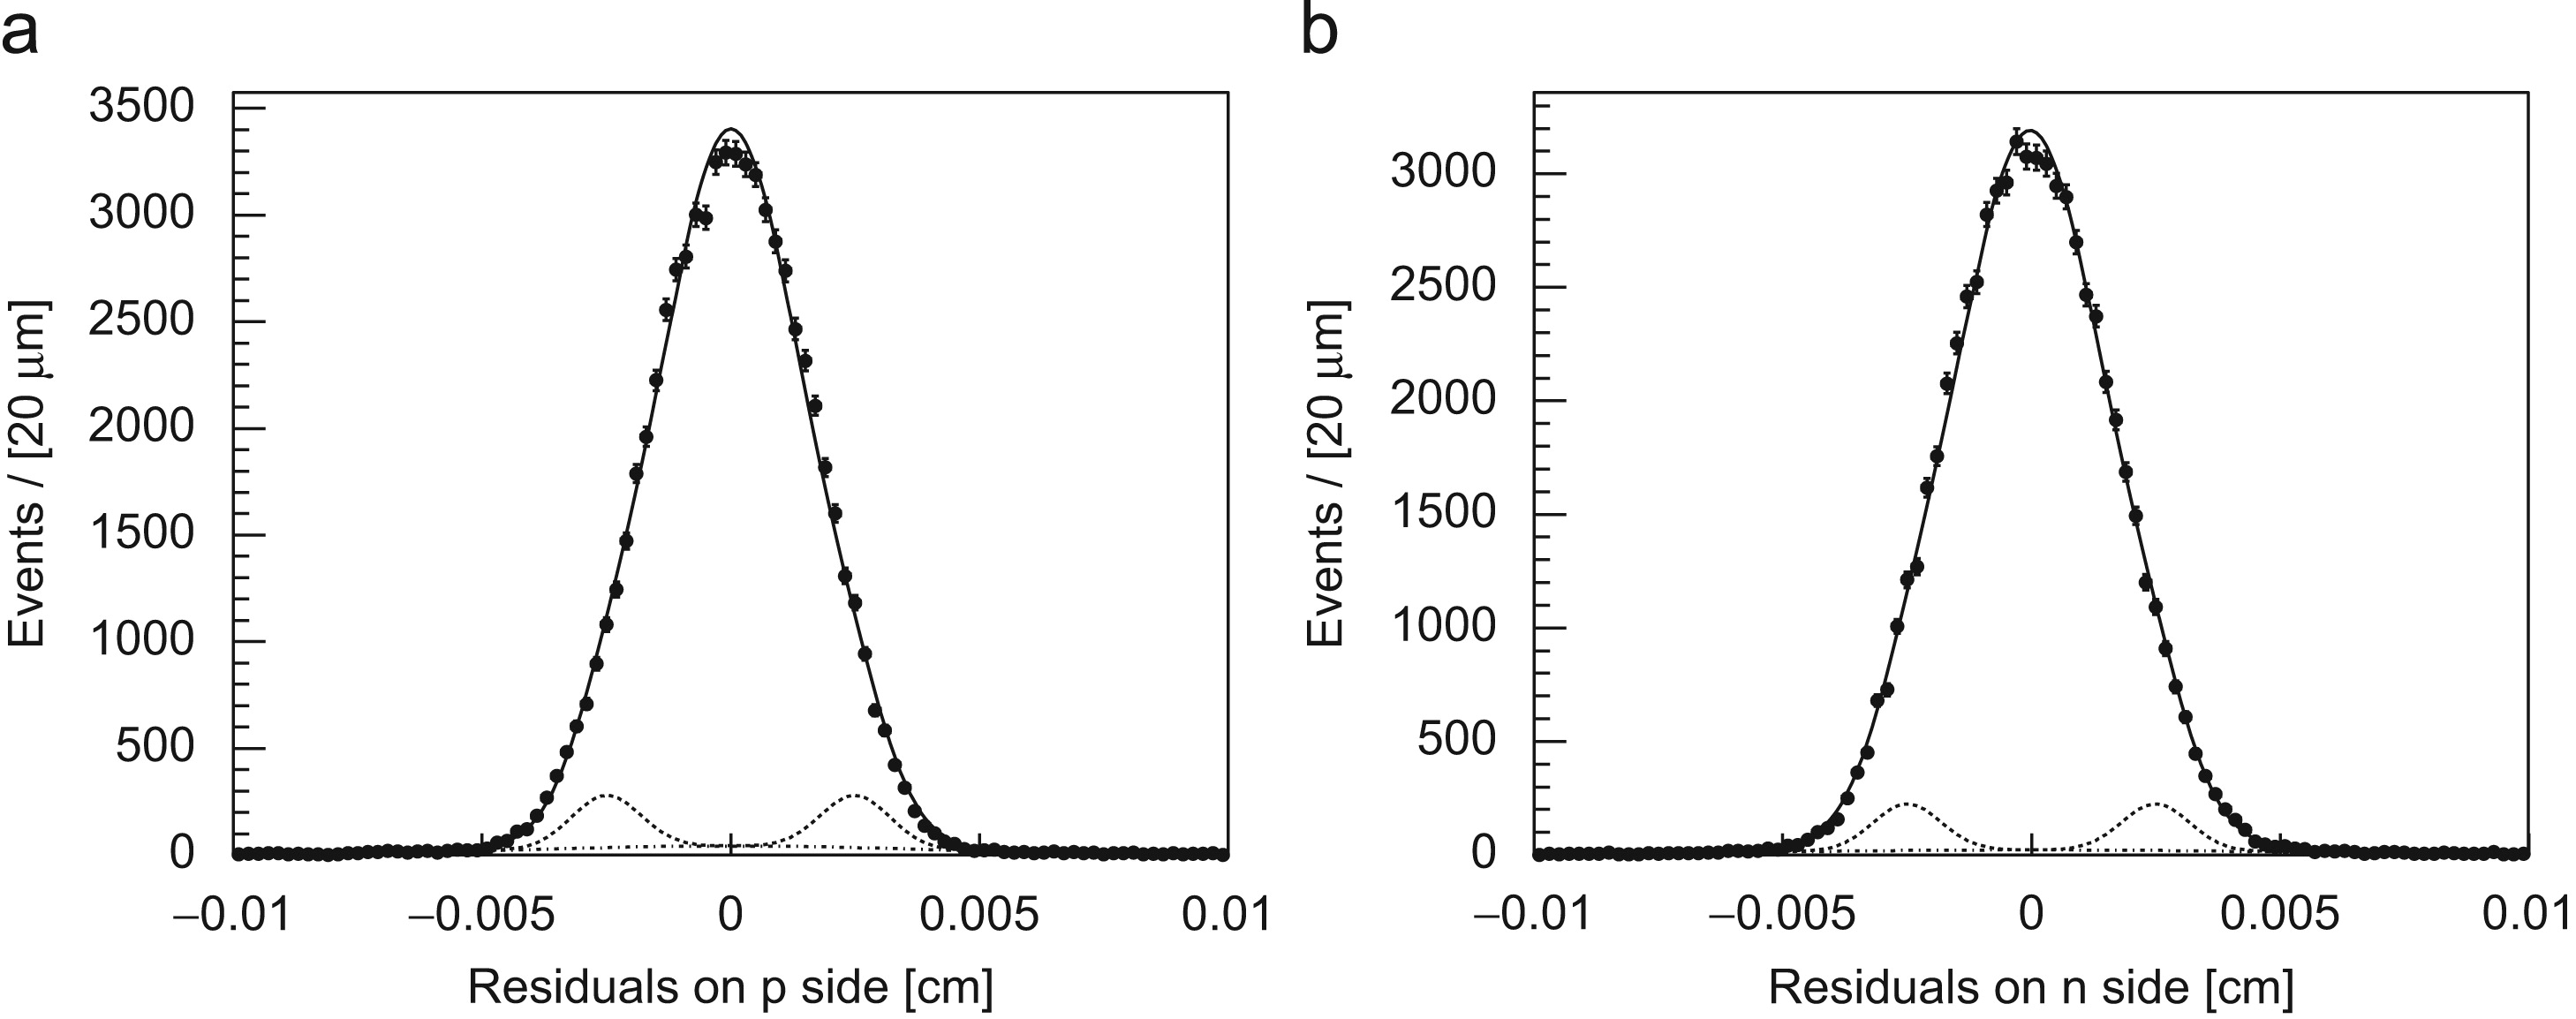
\includegraphics[width=1.0\textwidth]{striplets_residuals.jpg}
\caption{\label{fig:striplets_residuals}Residual fit for the striplets as a DUT for (a) p-side and (b) n-side. Data are points.  The solid  line 
is the   fit function  given in Equation~\ref{eq:res_pdf}; the dot-dashed line is the outlier Gaussian 
contribution, while the dashed line is all but the core Gaussian.}
\end{figure}

The fit results indicated that, once the dead strips are removed, the outlier component is negligible. 
On the contrary, about 7\% of the data were described by the double Gaussian component.

The intrinsic resolution was obtained using Equation~\ref{eq:res}, where $\sigma_{res}$ is taken as 
the width of the narrow core Gaussian of the fit function. We found an intrinsic resolution of 
13.6~$\mu$m for the $p-$side and 14.1~$\mu$m or the $n-$side, slightly better than the digital 
resolution for a 50~$\mu$m readout pitch and in agreement with the expected values for strip detectors with similar $S/N$.

\subsubsection{Spatial Resolution as a Function of the Track Angle}

The spatial resolution of striplets was studied as a function of of the incident track angle; 
the results are reported in Figure~\ref{fig:cluster_rotation}, where the average cluster size 
is shown too.

\begin{figure}[!htbp]
\centering
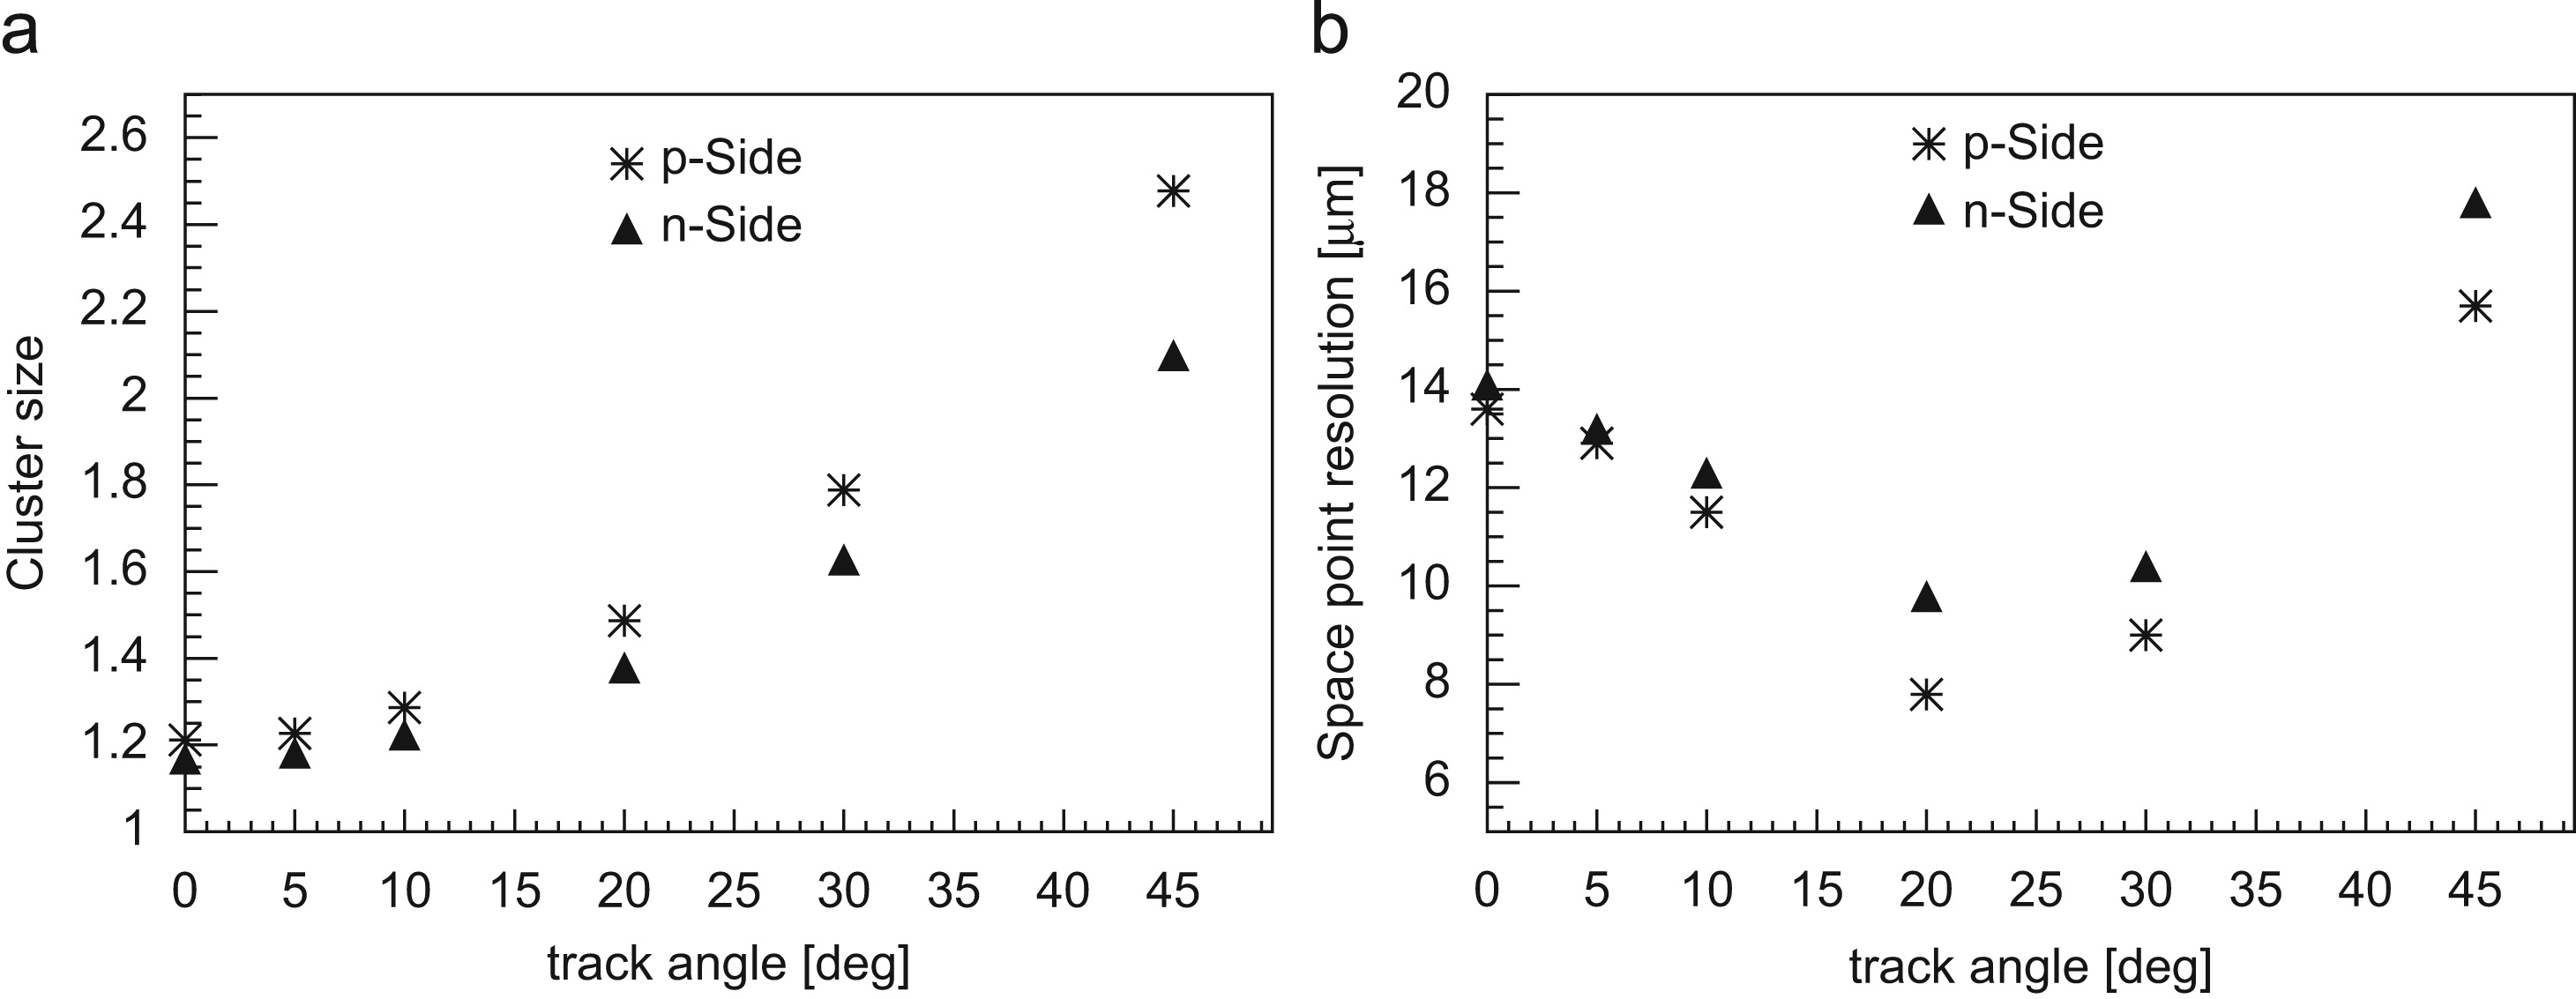
\includegraphics[width=1.0\textwidth]{cluster_rotation.jpg}
\caption{\label{fig:cluster_rotation}(a) Average cluster size for the striplets as a function of track angle. (b) Resolutions for the striplets as a function of track angle.}
\end{figure}

The average cluster size increases and therefore the resolutions improve considerably as a function 
of the incident angle up to 30$^{\circ}$, after which the performance degrades. This is 
in good agreement with expectations~\cite{TURCHETTA}. At 45$^{\circ}$ the resolution is 
about 20\% worse than that at normal incidence. 

Cluster size was smaller for $n-$side than $p-$side for all angles investigated; as a consequence 
the resolution was worse for $n-$side than $p-$side. This is the result of higher noise, higher 
threshold and limited ADC range for $n-$side (see Table~\ref{tab:FSSR2Calib}).

The residuals distributions as a function of the incident track angle are presented in 
Figure~\ref{fig:res_angles}.

\begin{figure}[!htpb]
\centering
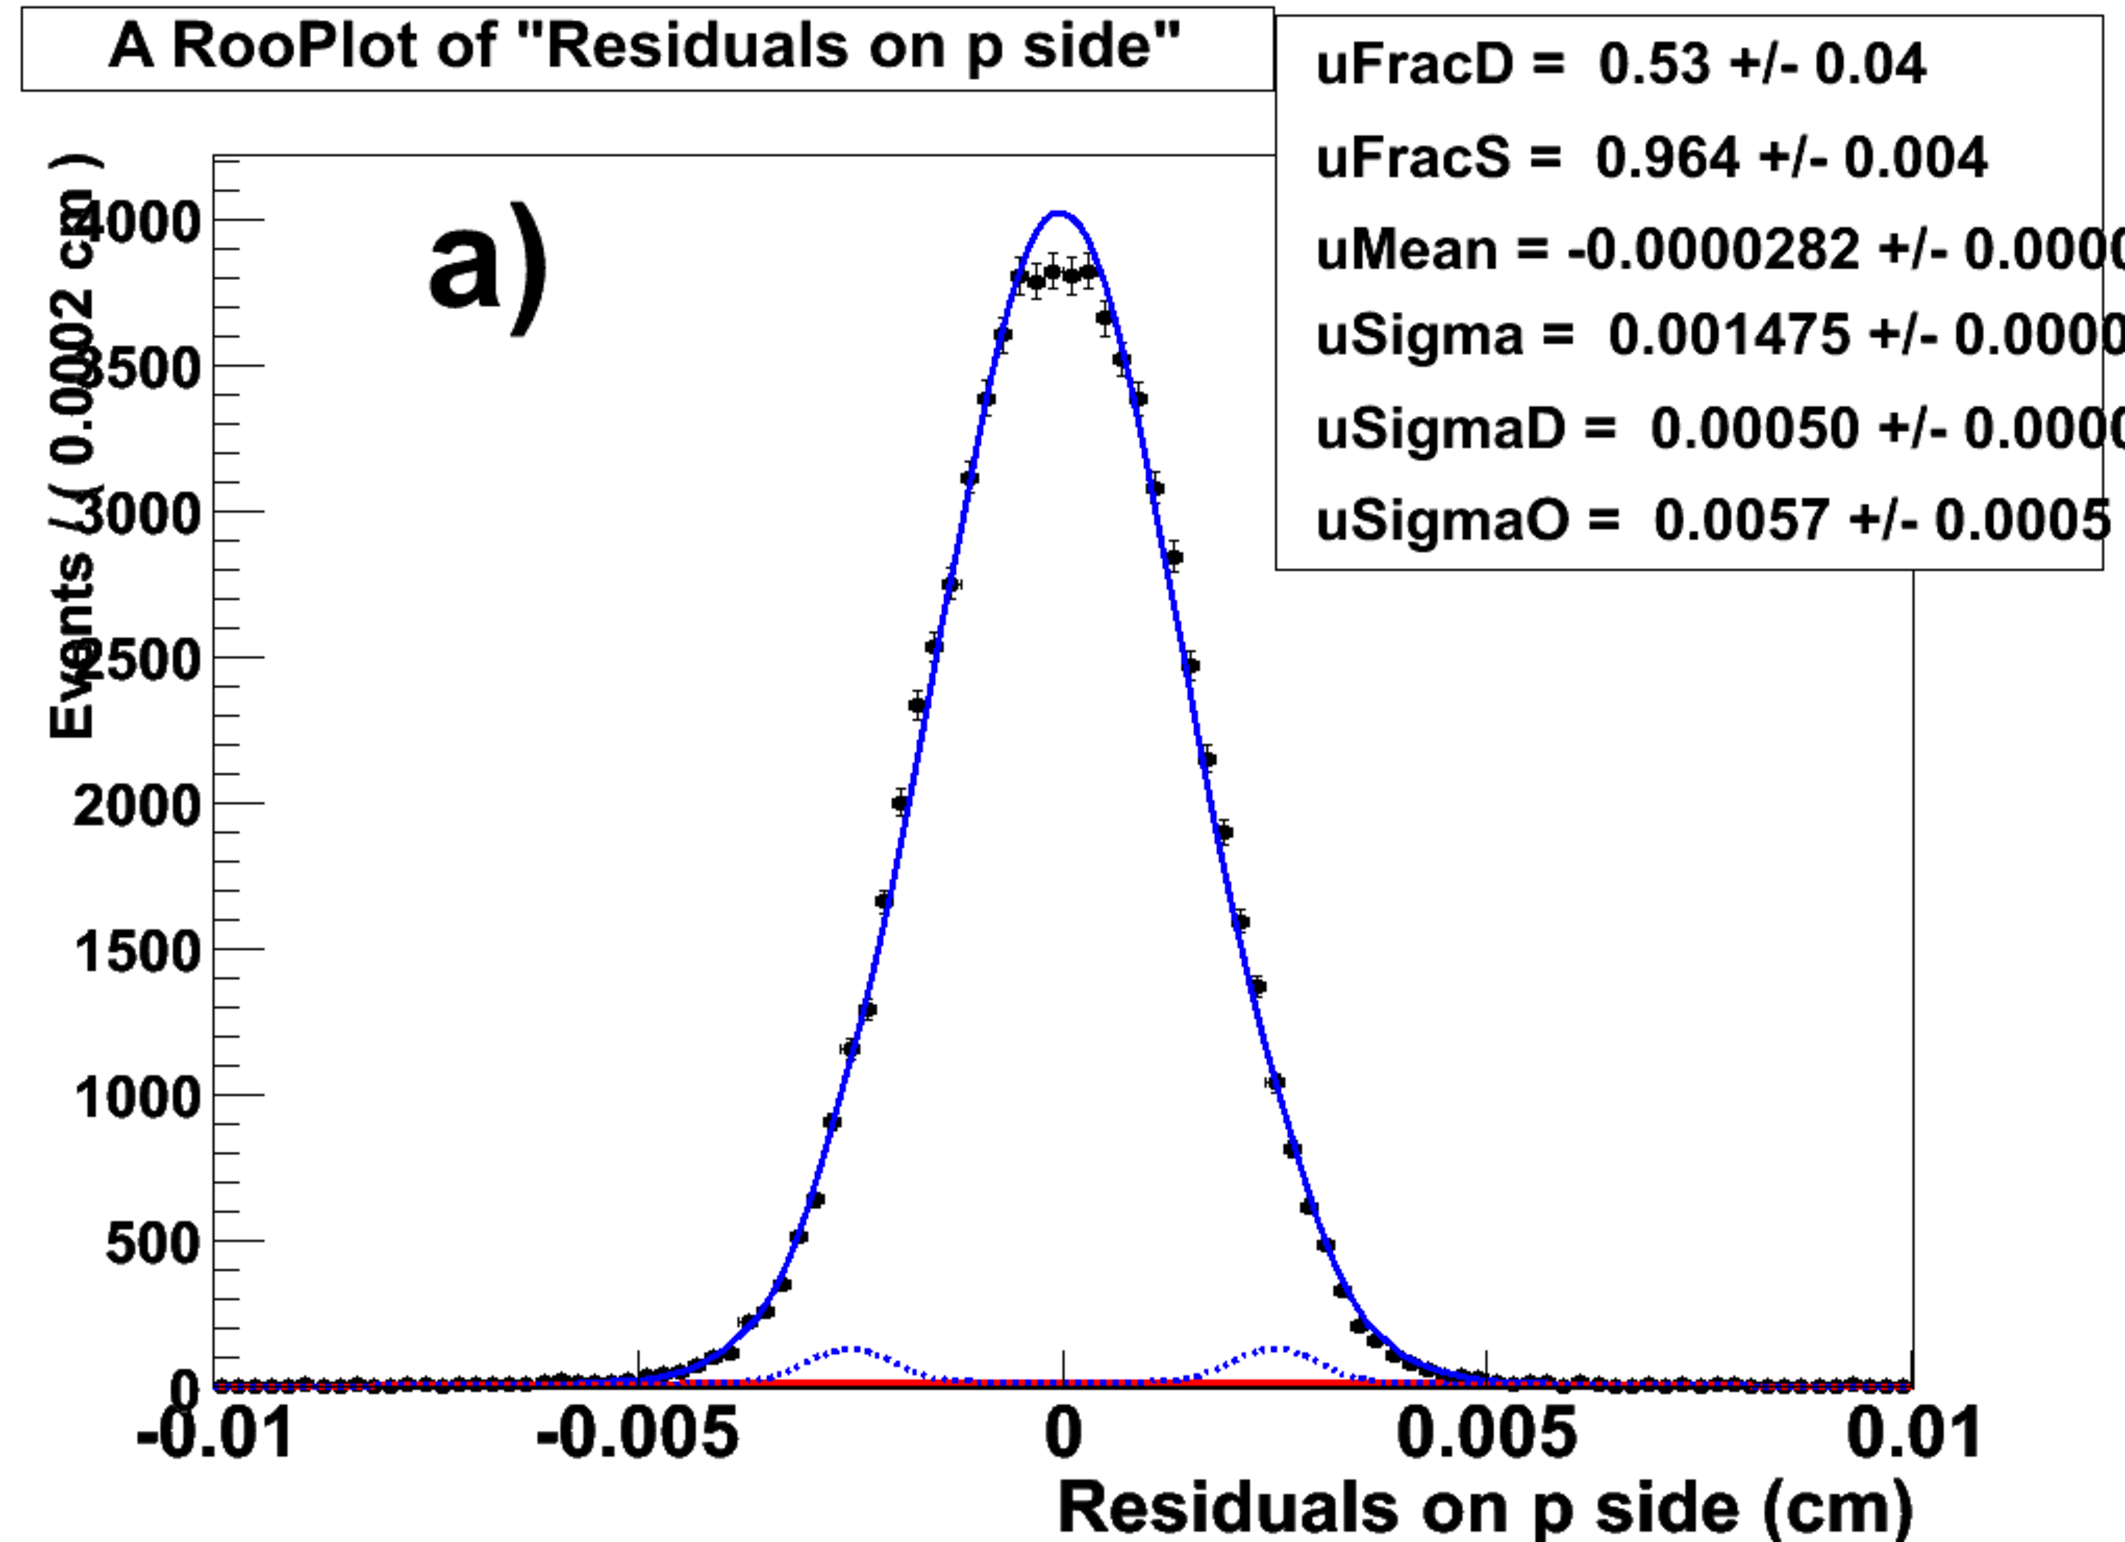
\includegraphics[width=0.39\textwidth]{res_pside_5deg.pdf}
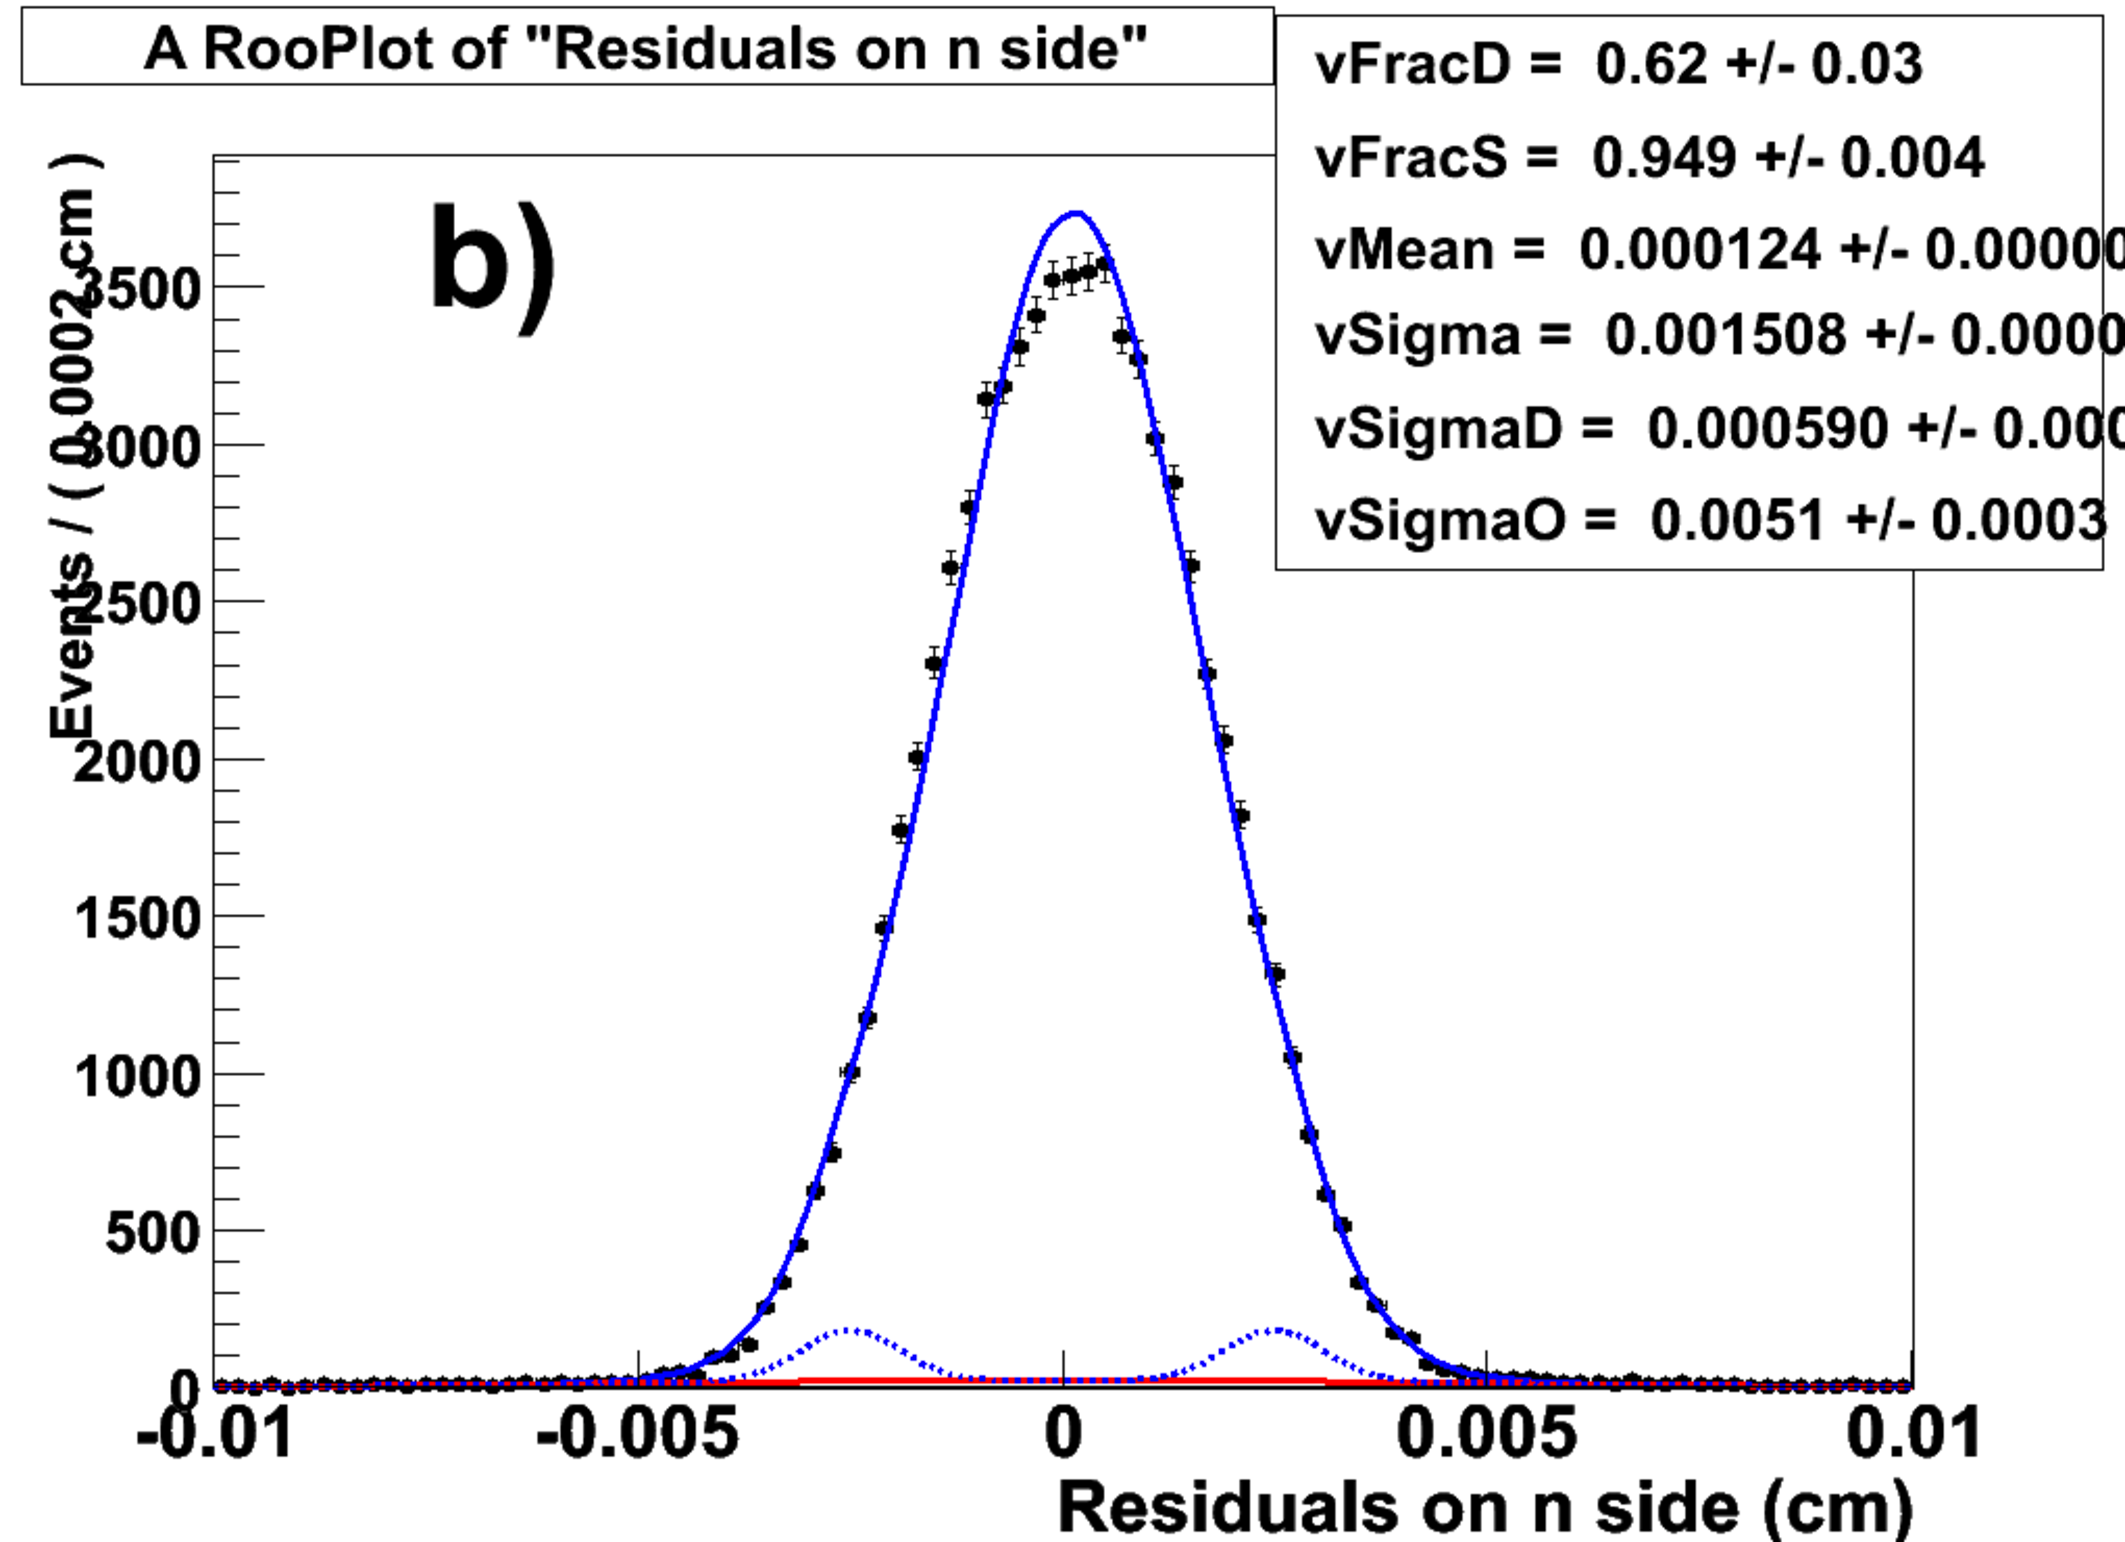
\includegraphics[width=0.39\textwidth]{res_nside_5deg.pdf}
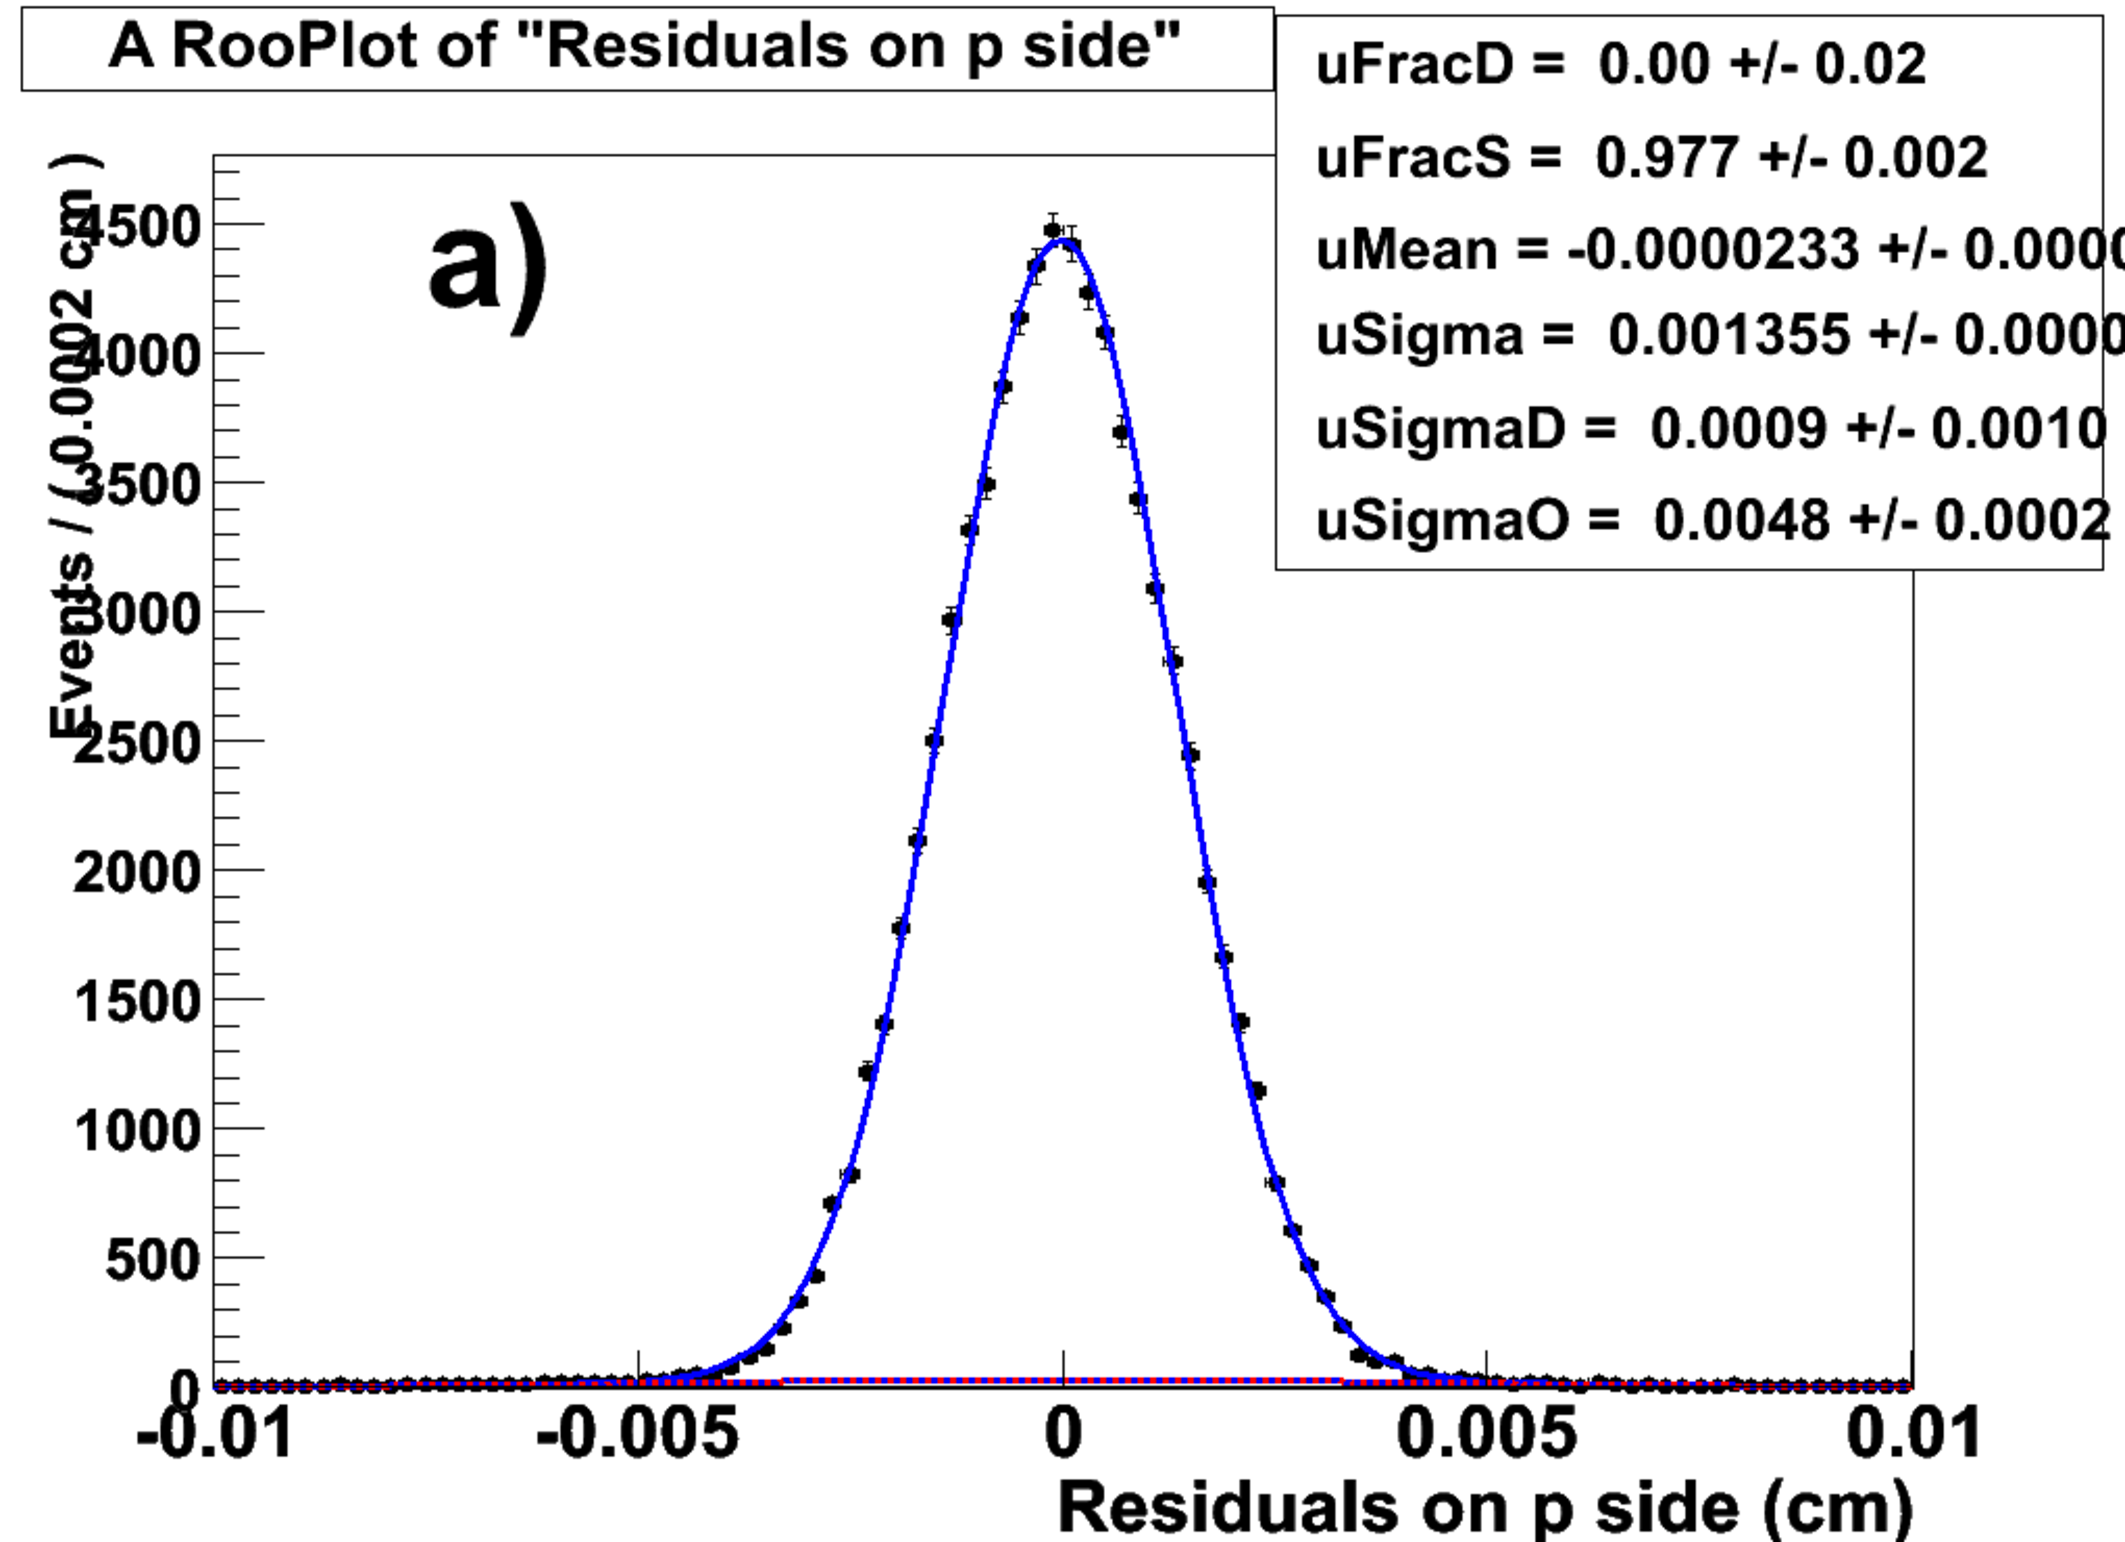
\includegraphics[width=0.39\textwidth]{res_pside_10deg.pdf}
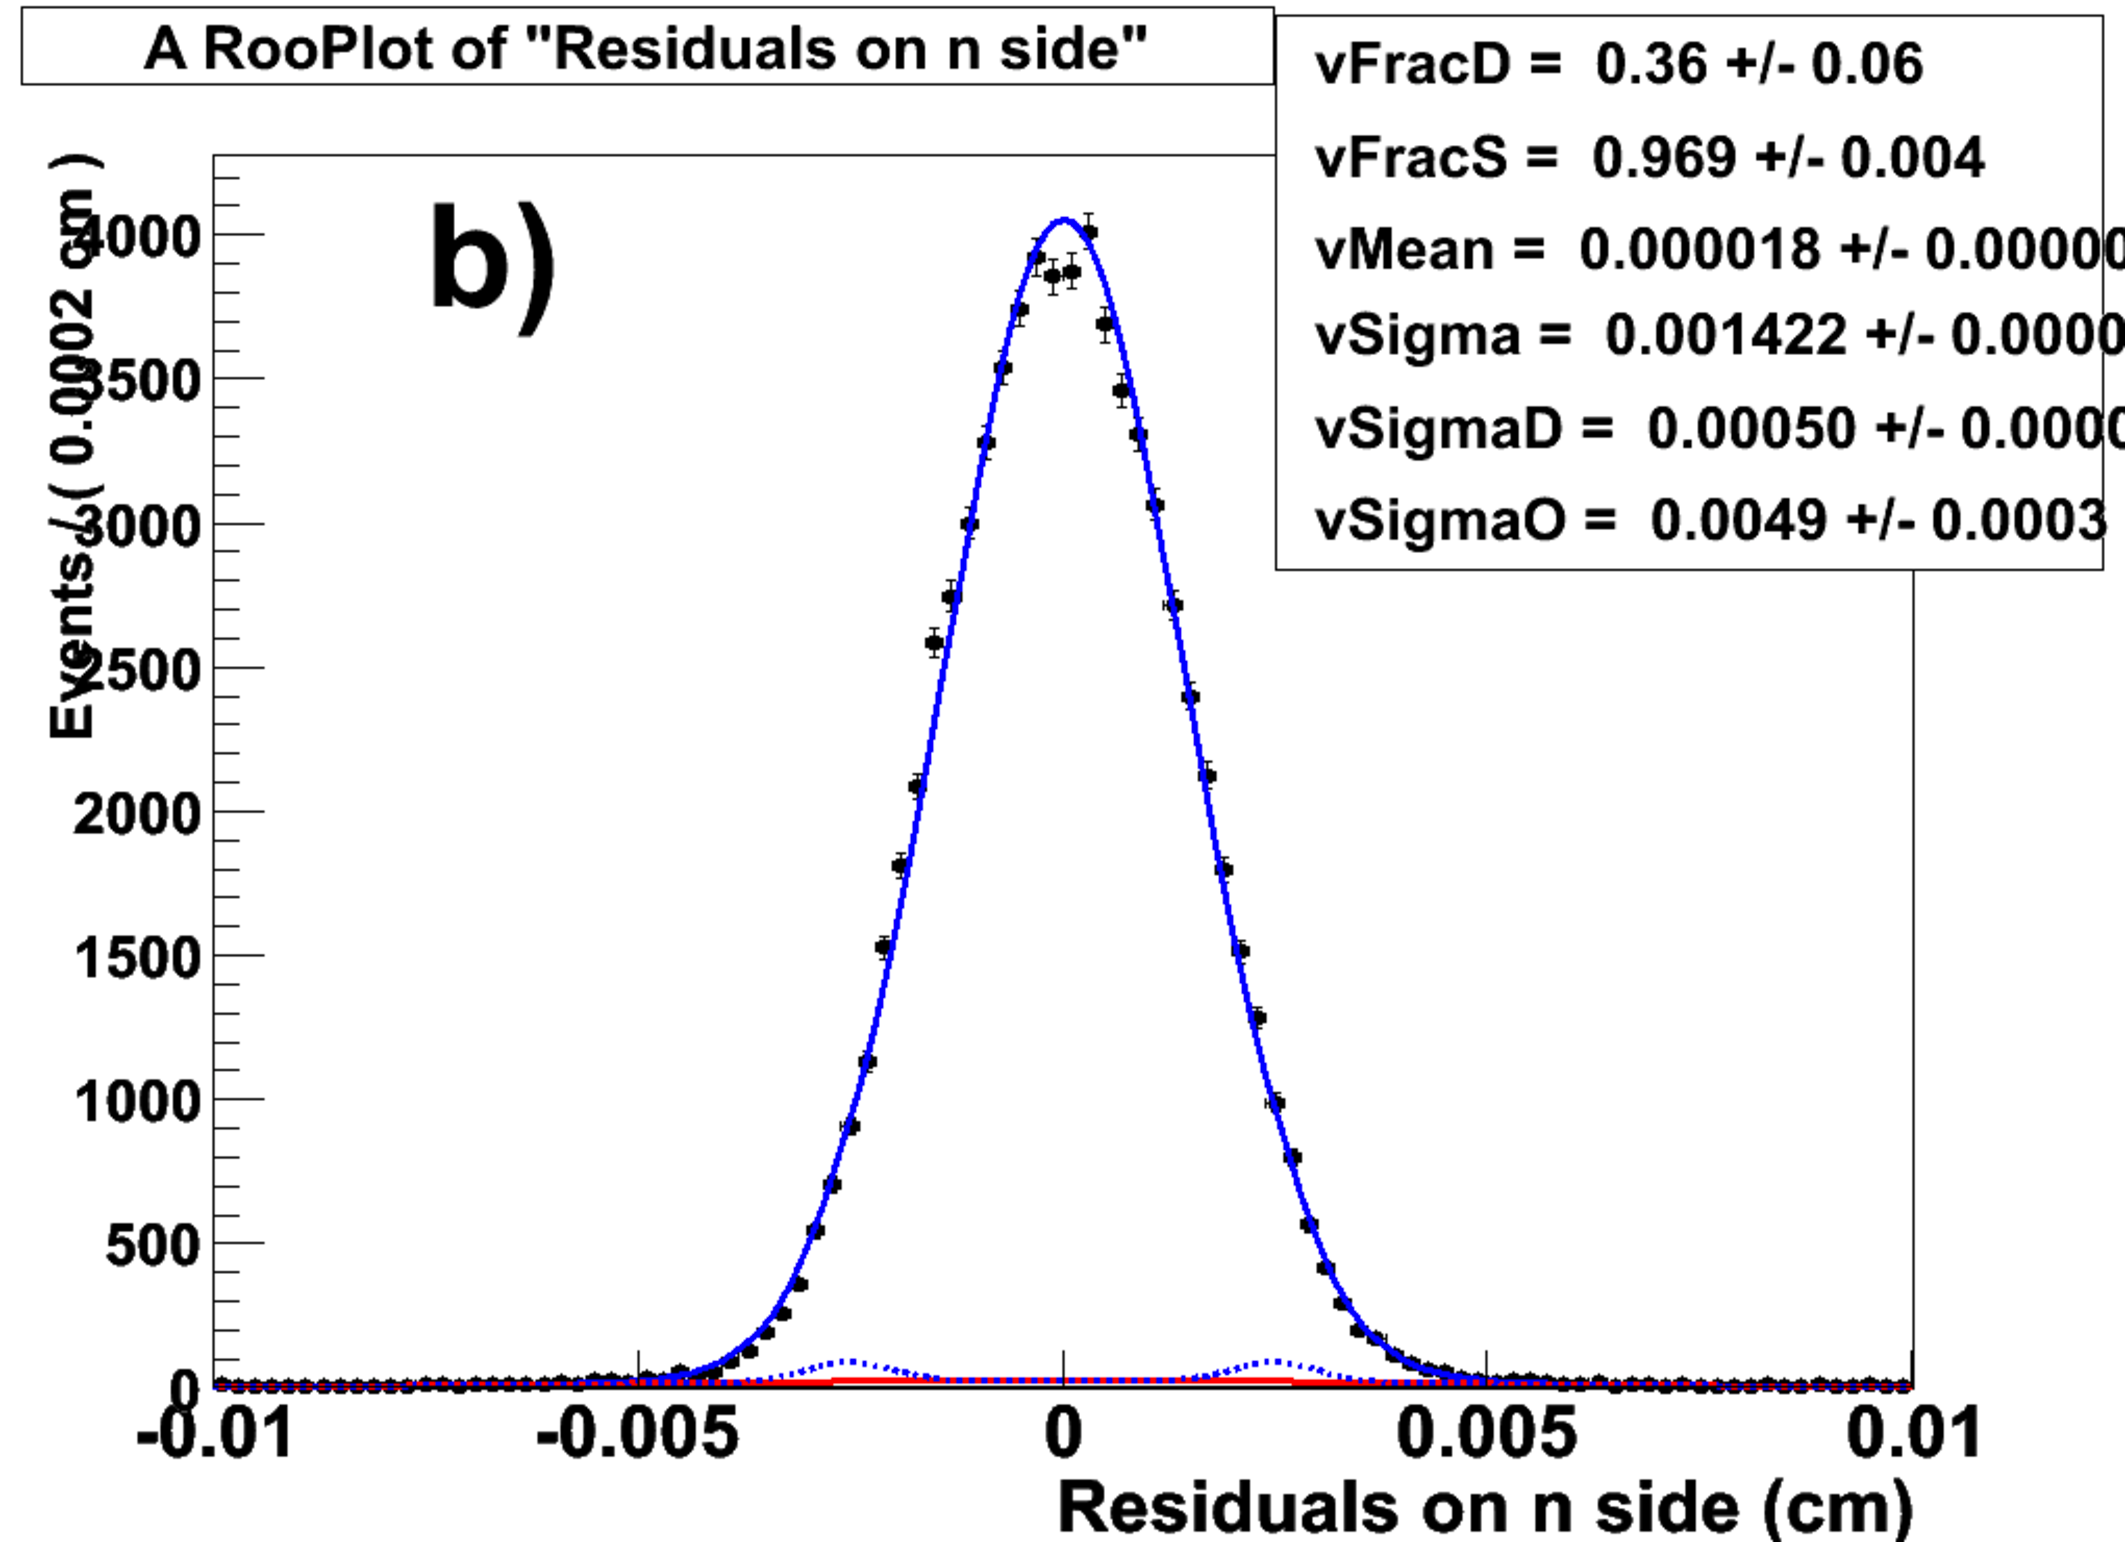
\includegraphics[width=0.39\textwidth]{res_nside_10deg.pdf}
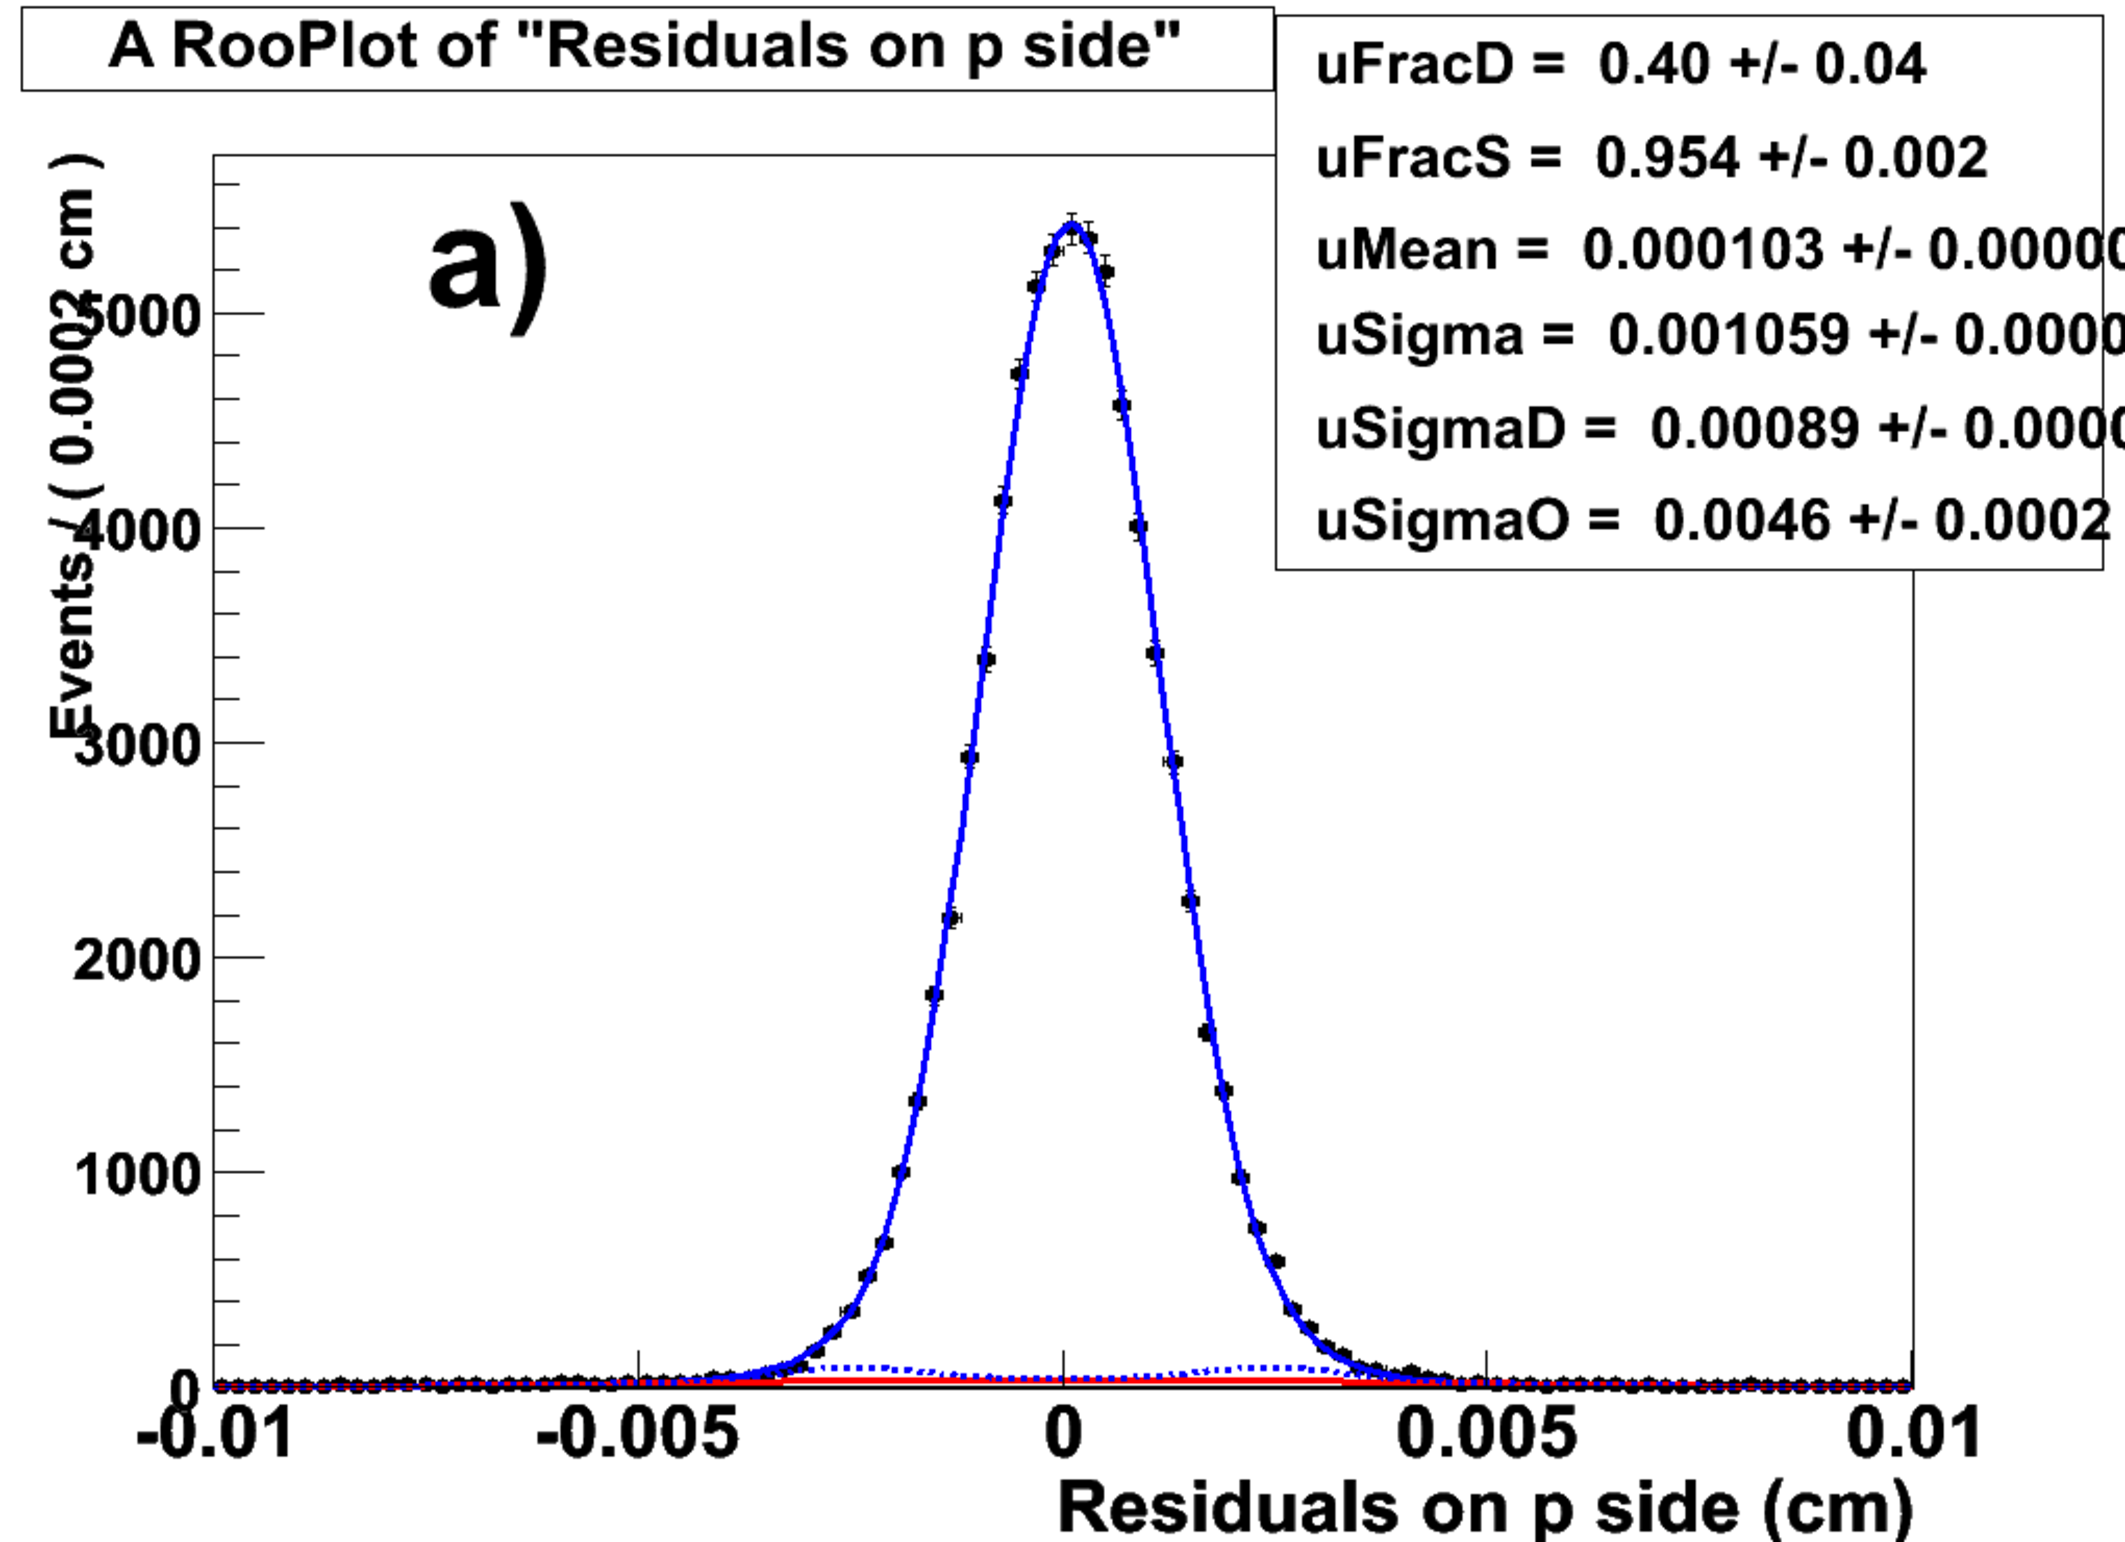
\includegraphics[width=0.39\textwidth]{res_pside_20deg.pdf}
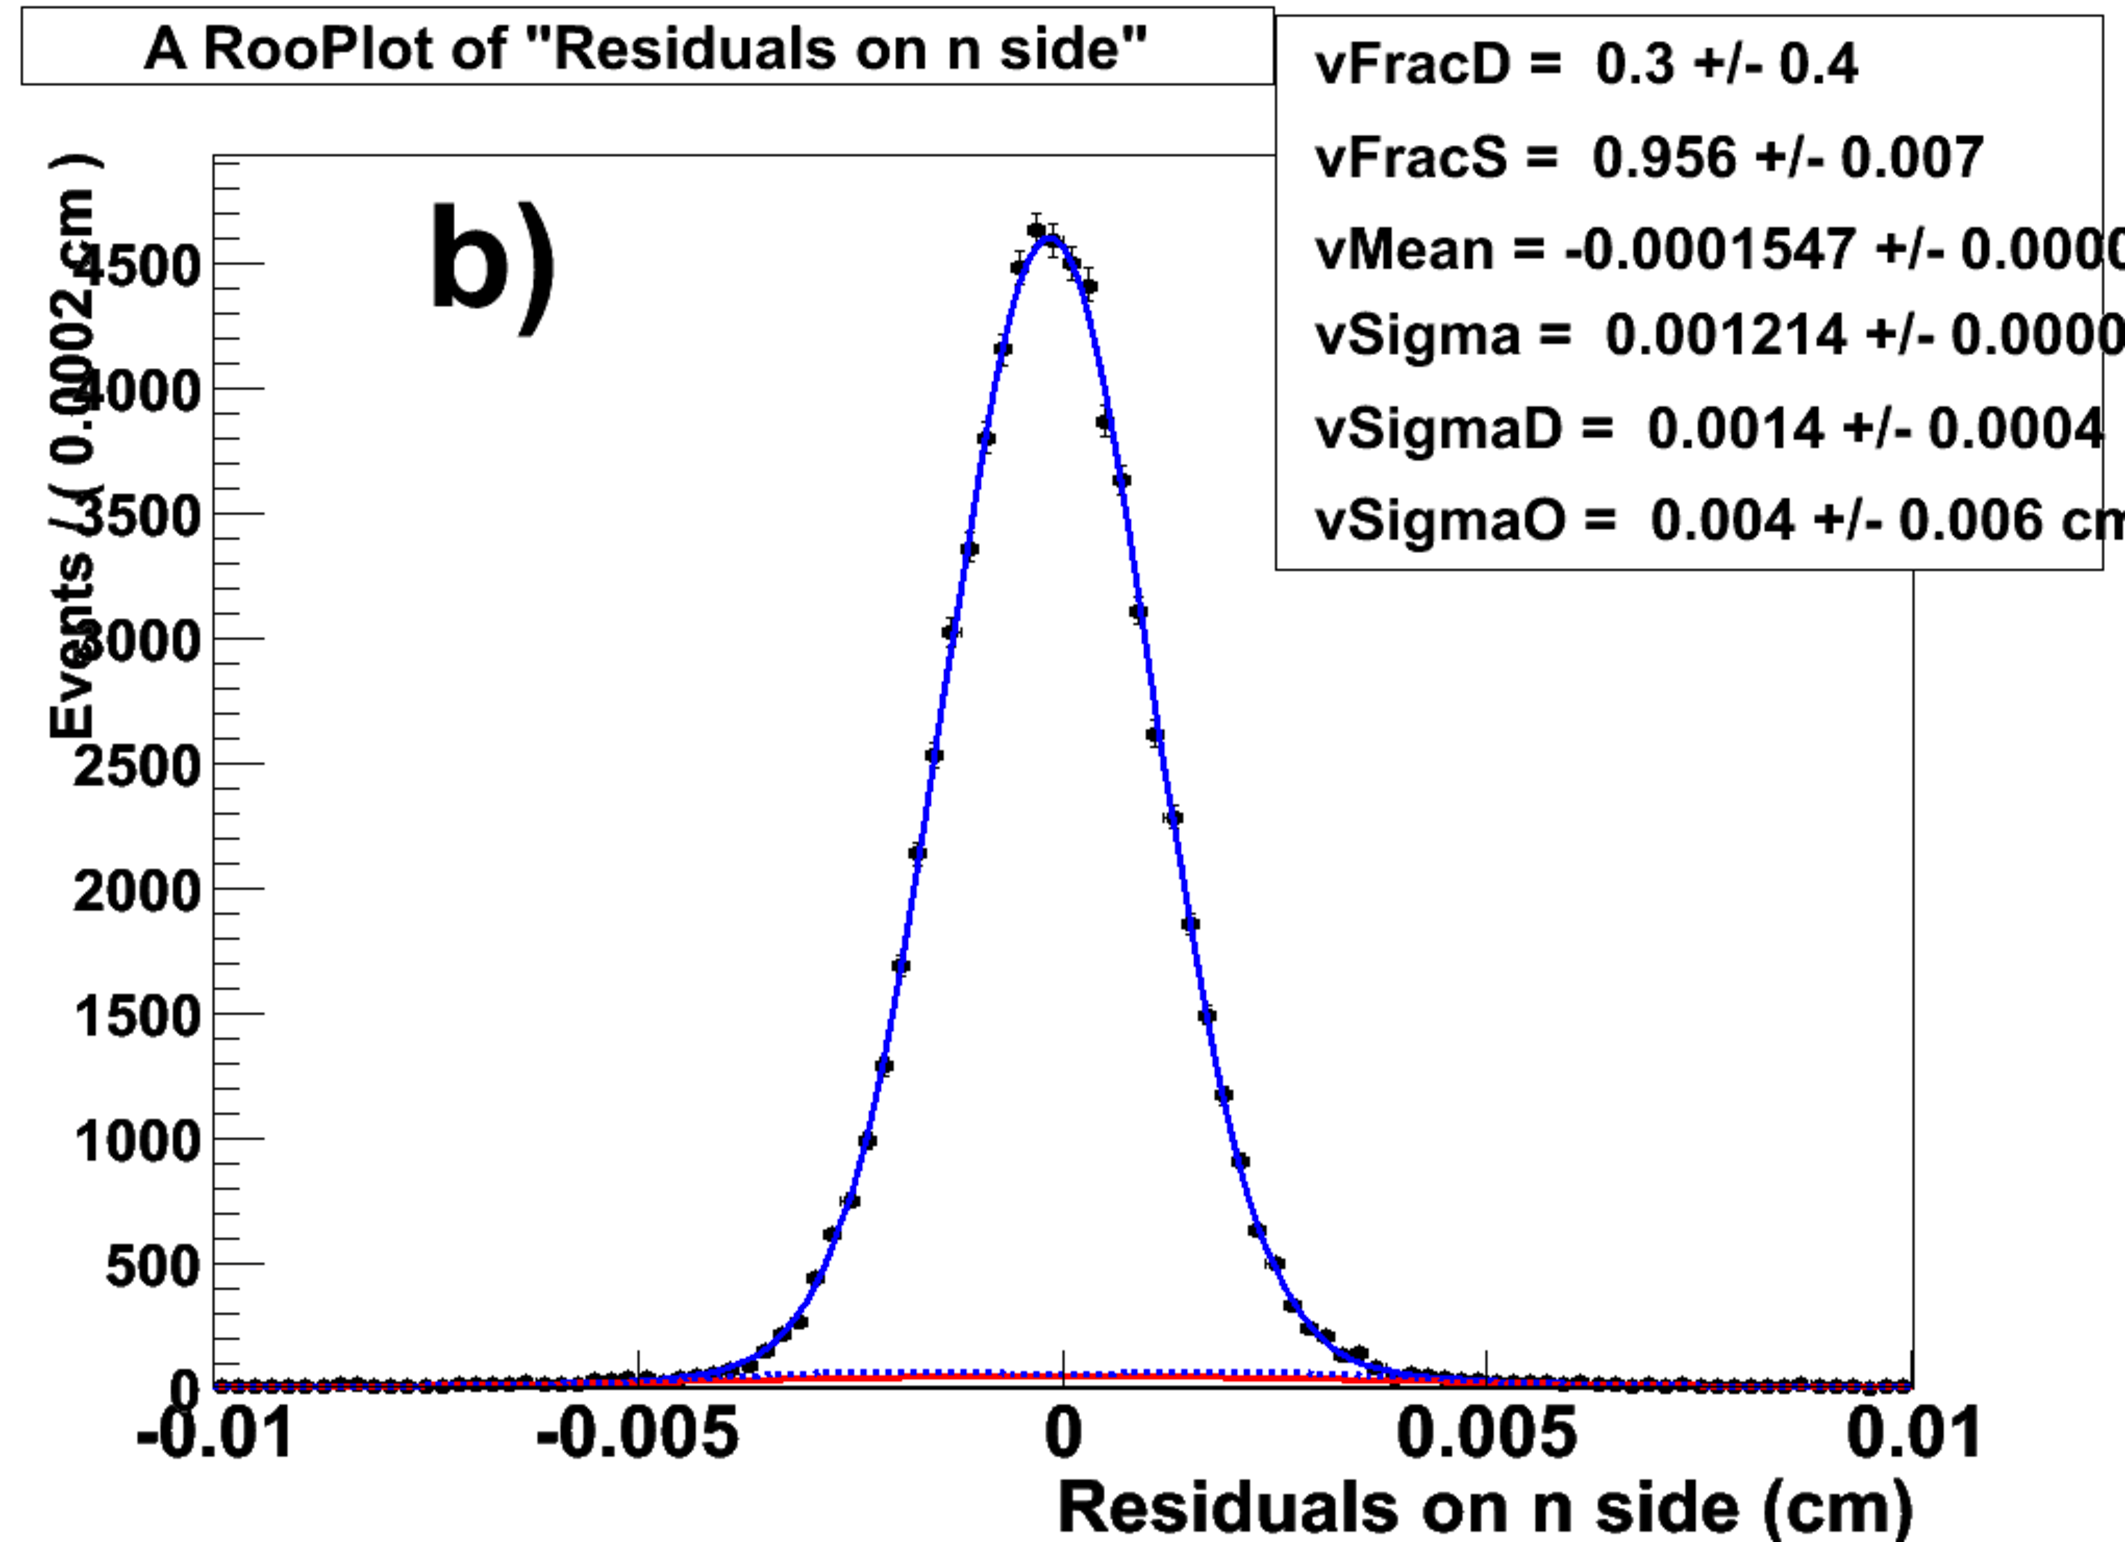
\includegraphics[width=0.39\textwidth]{res_nside_20deg.pdf}
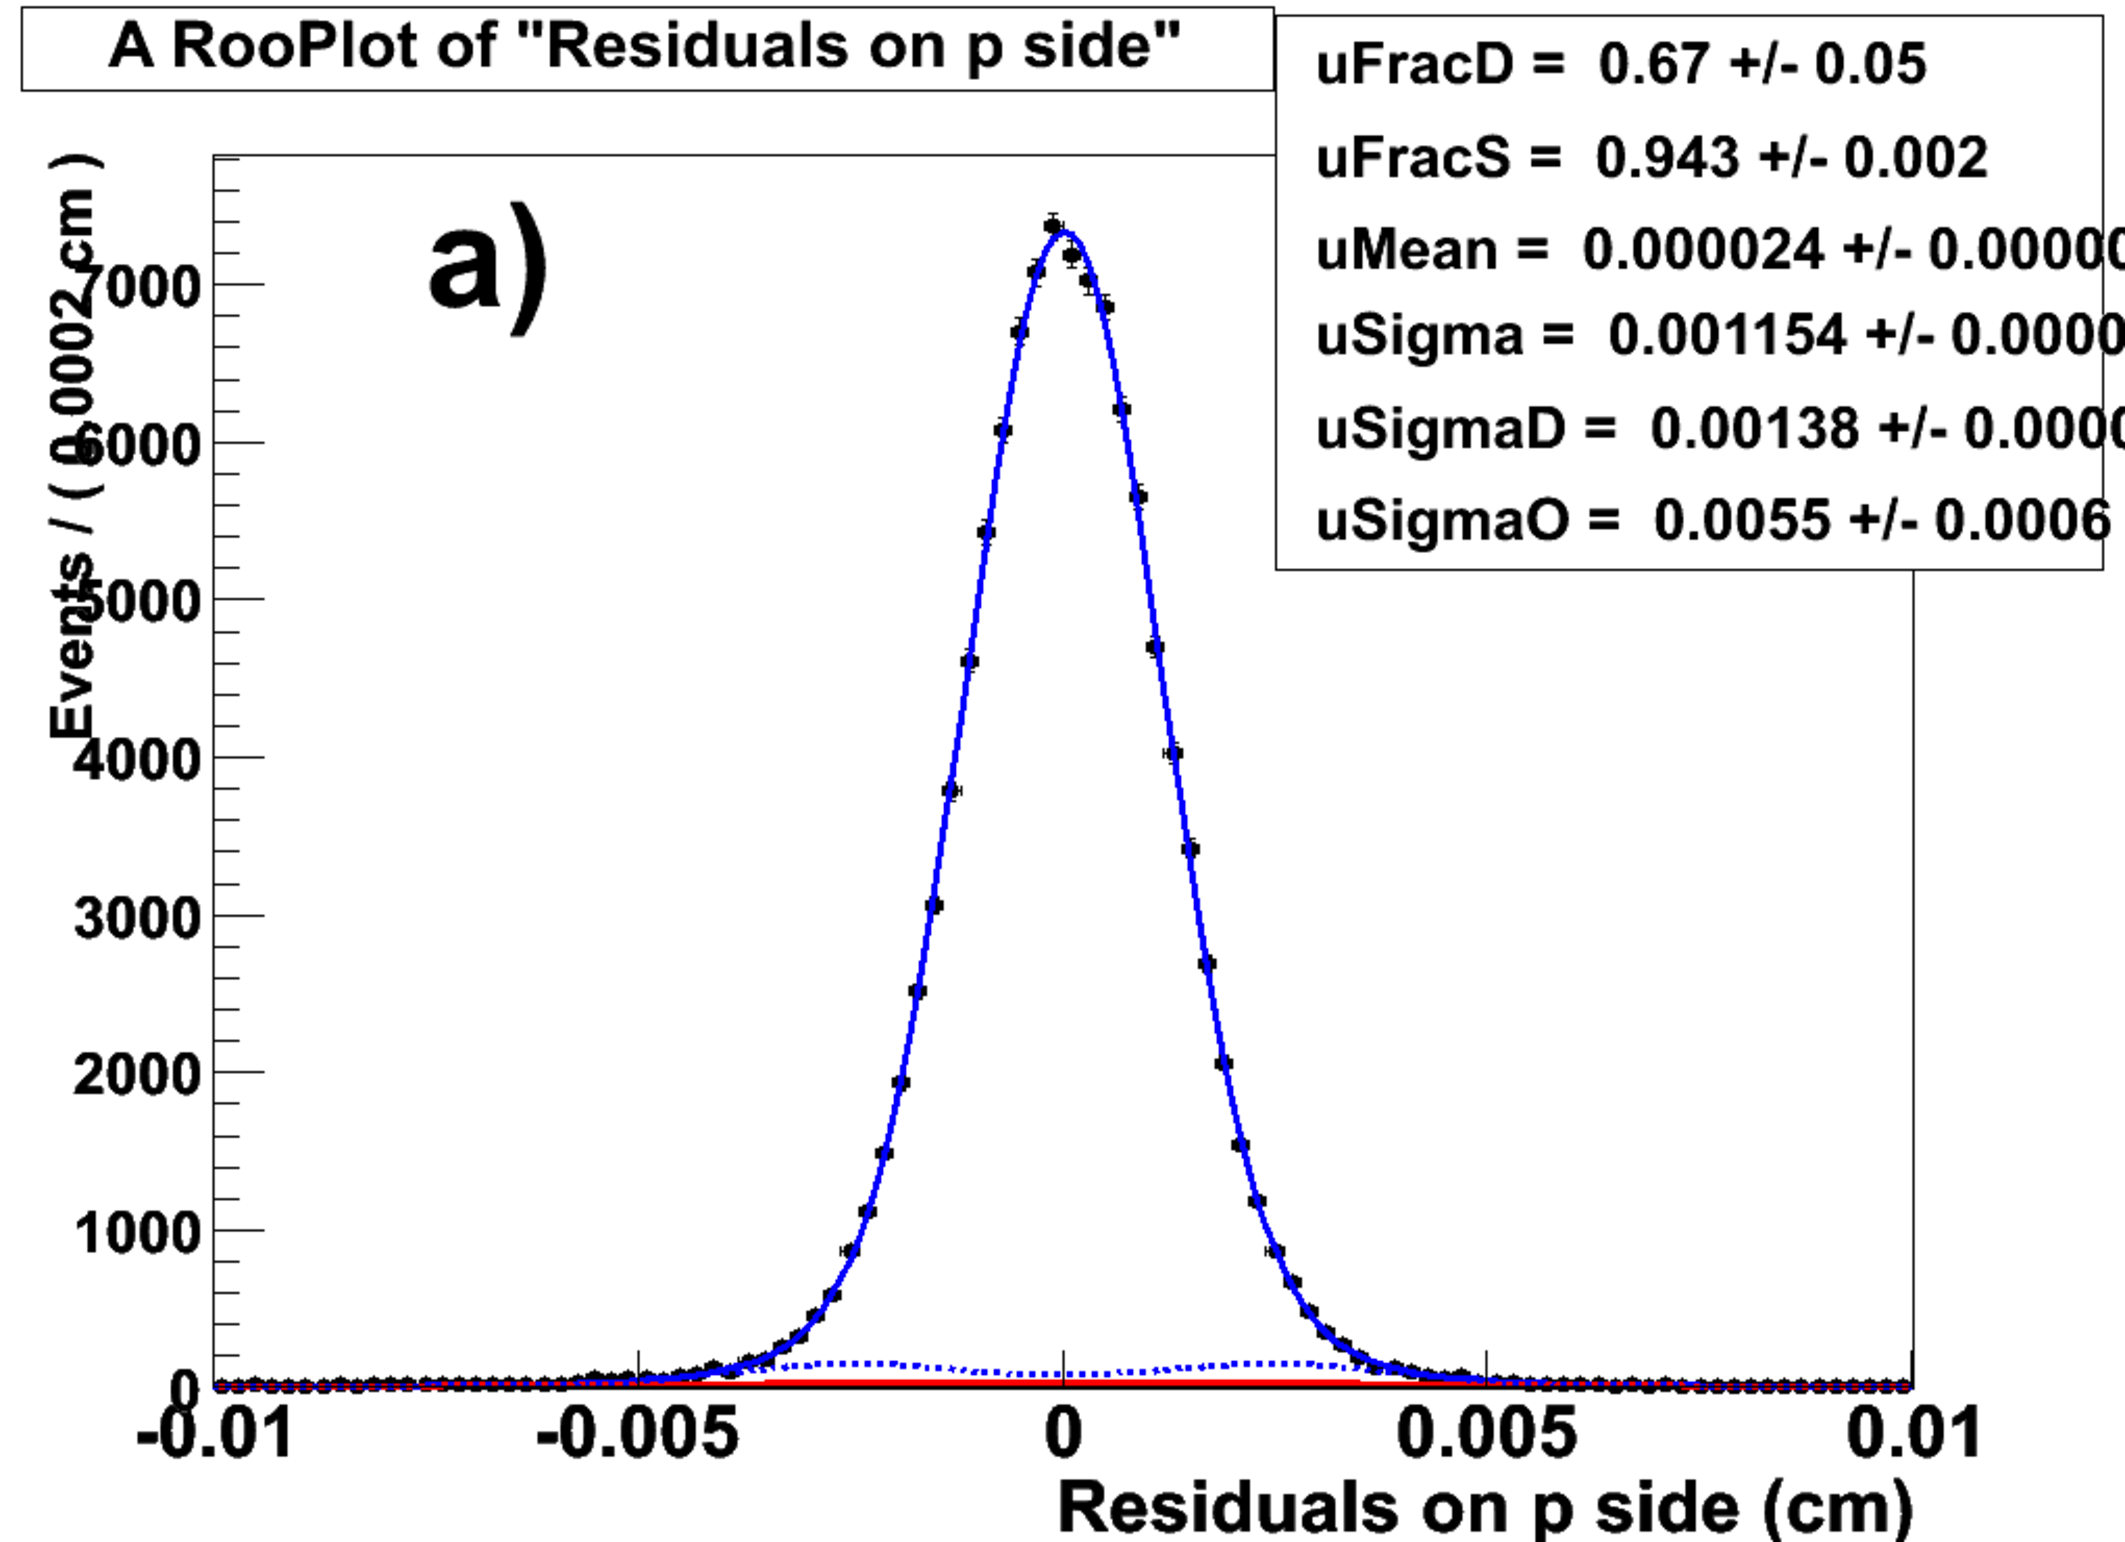
\includegraphics[width=0.39\textwidth]{res_pside_30deg.pdf}
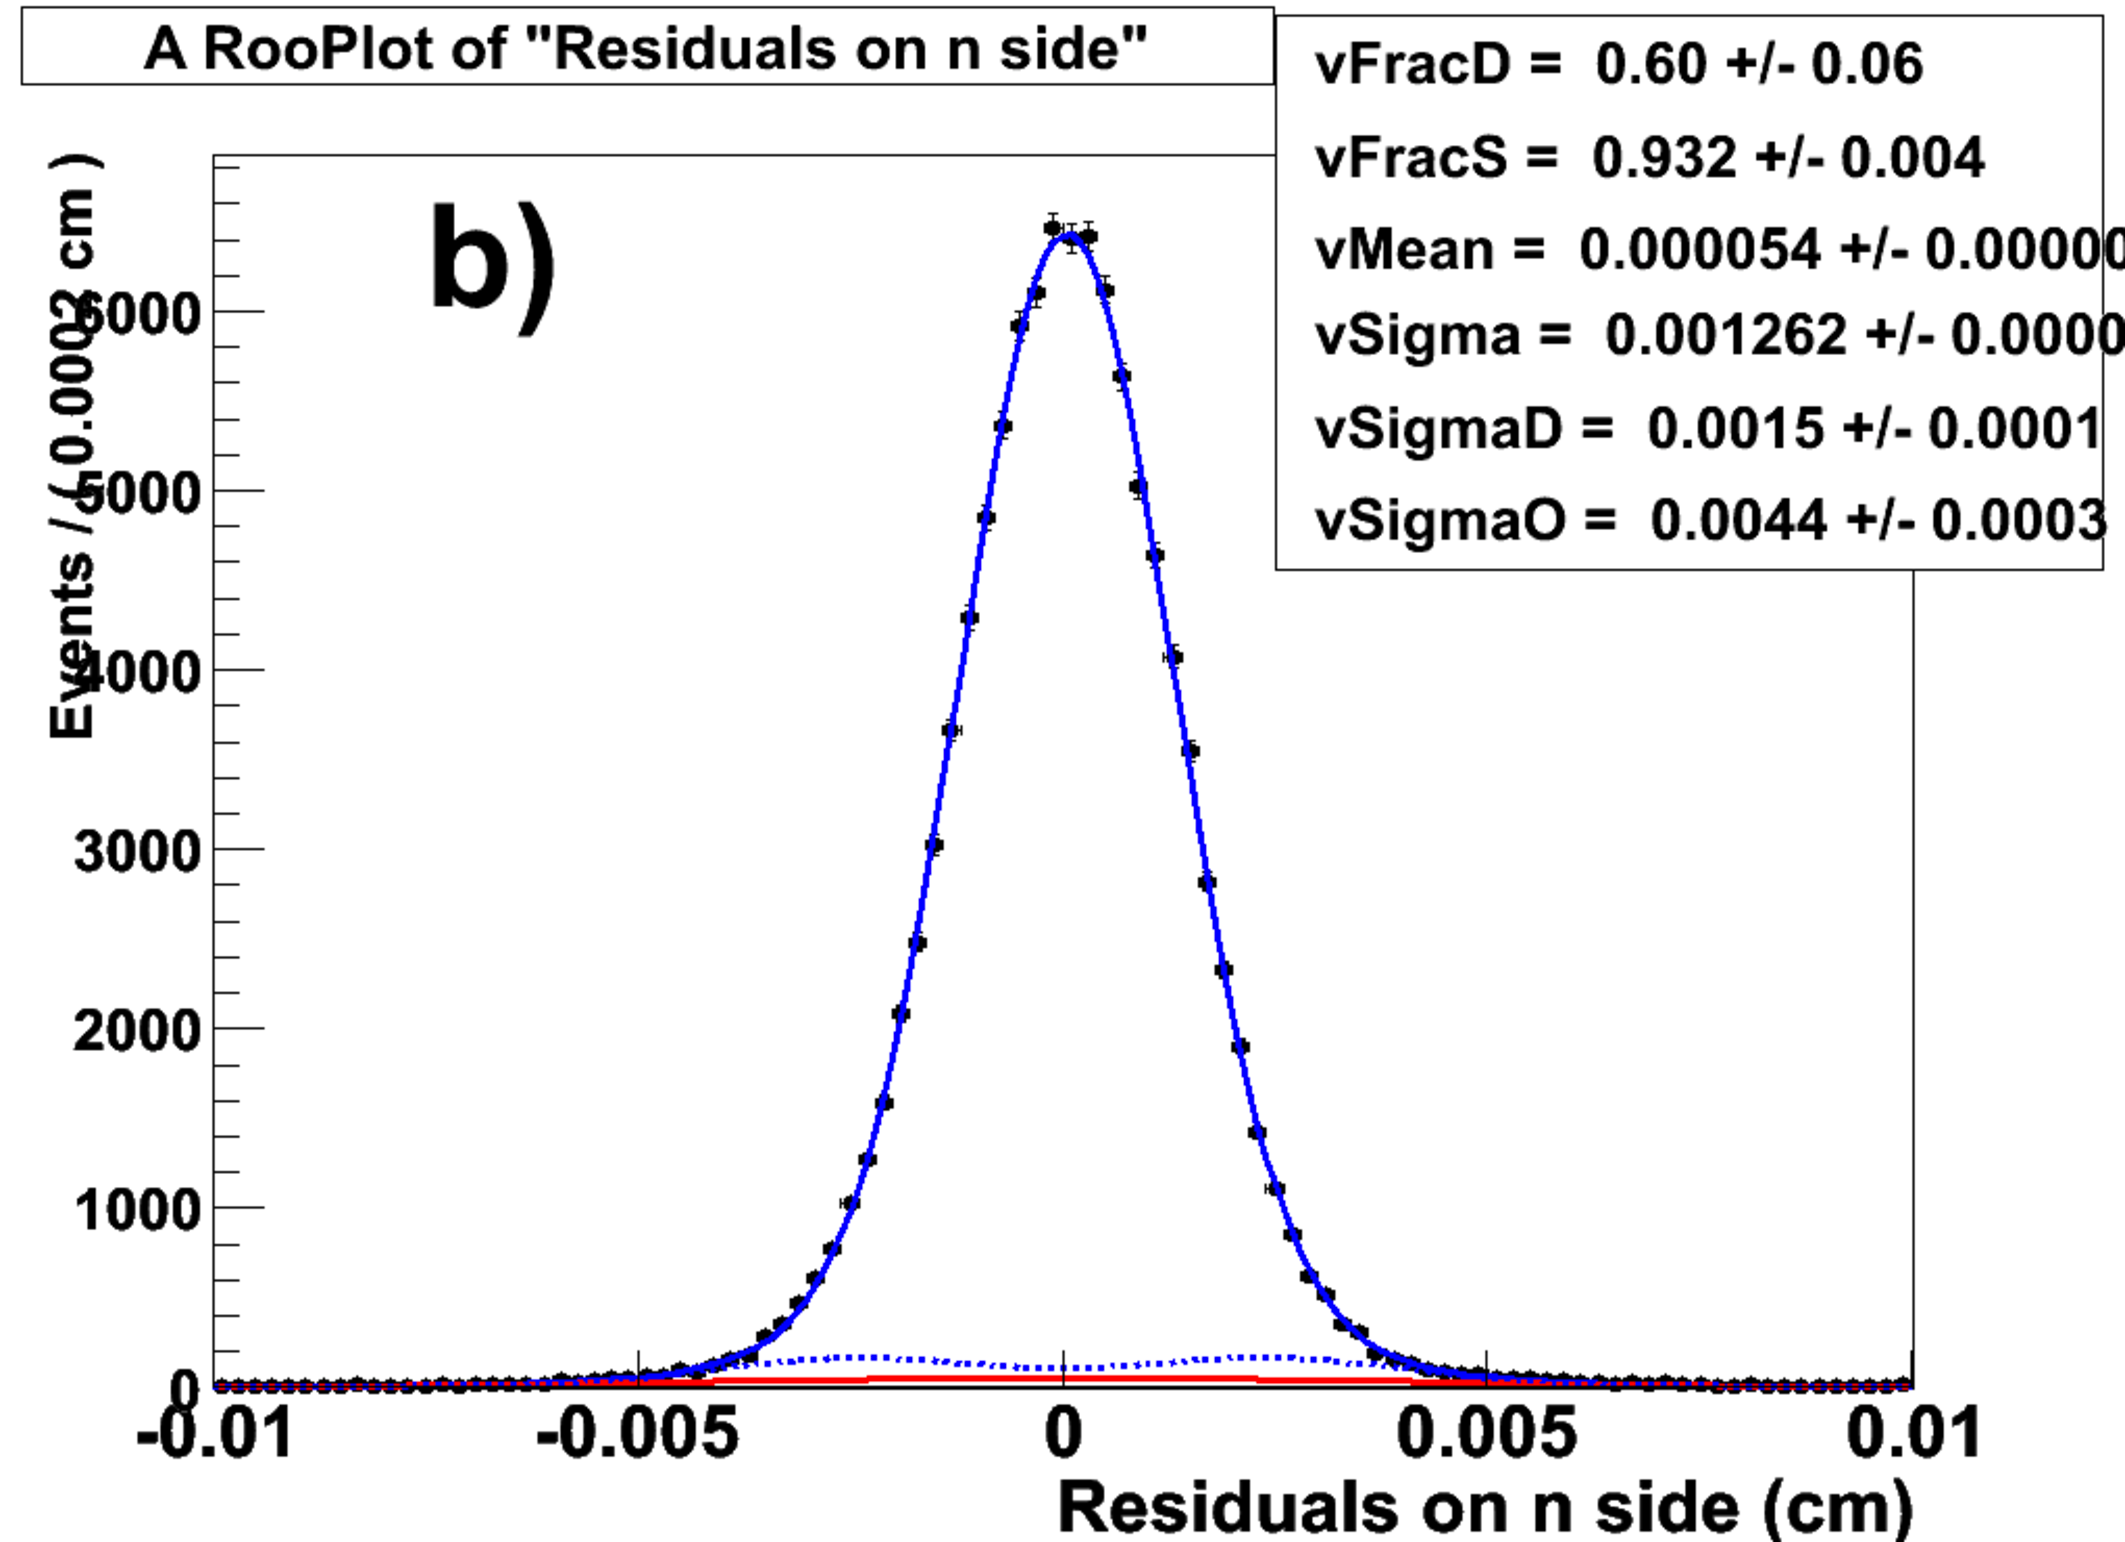
\includegraphics[width=0.39\textwidth]{res_nside_30deg.pdf}
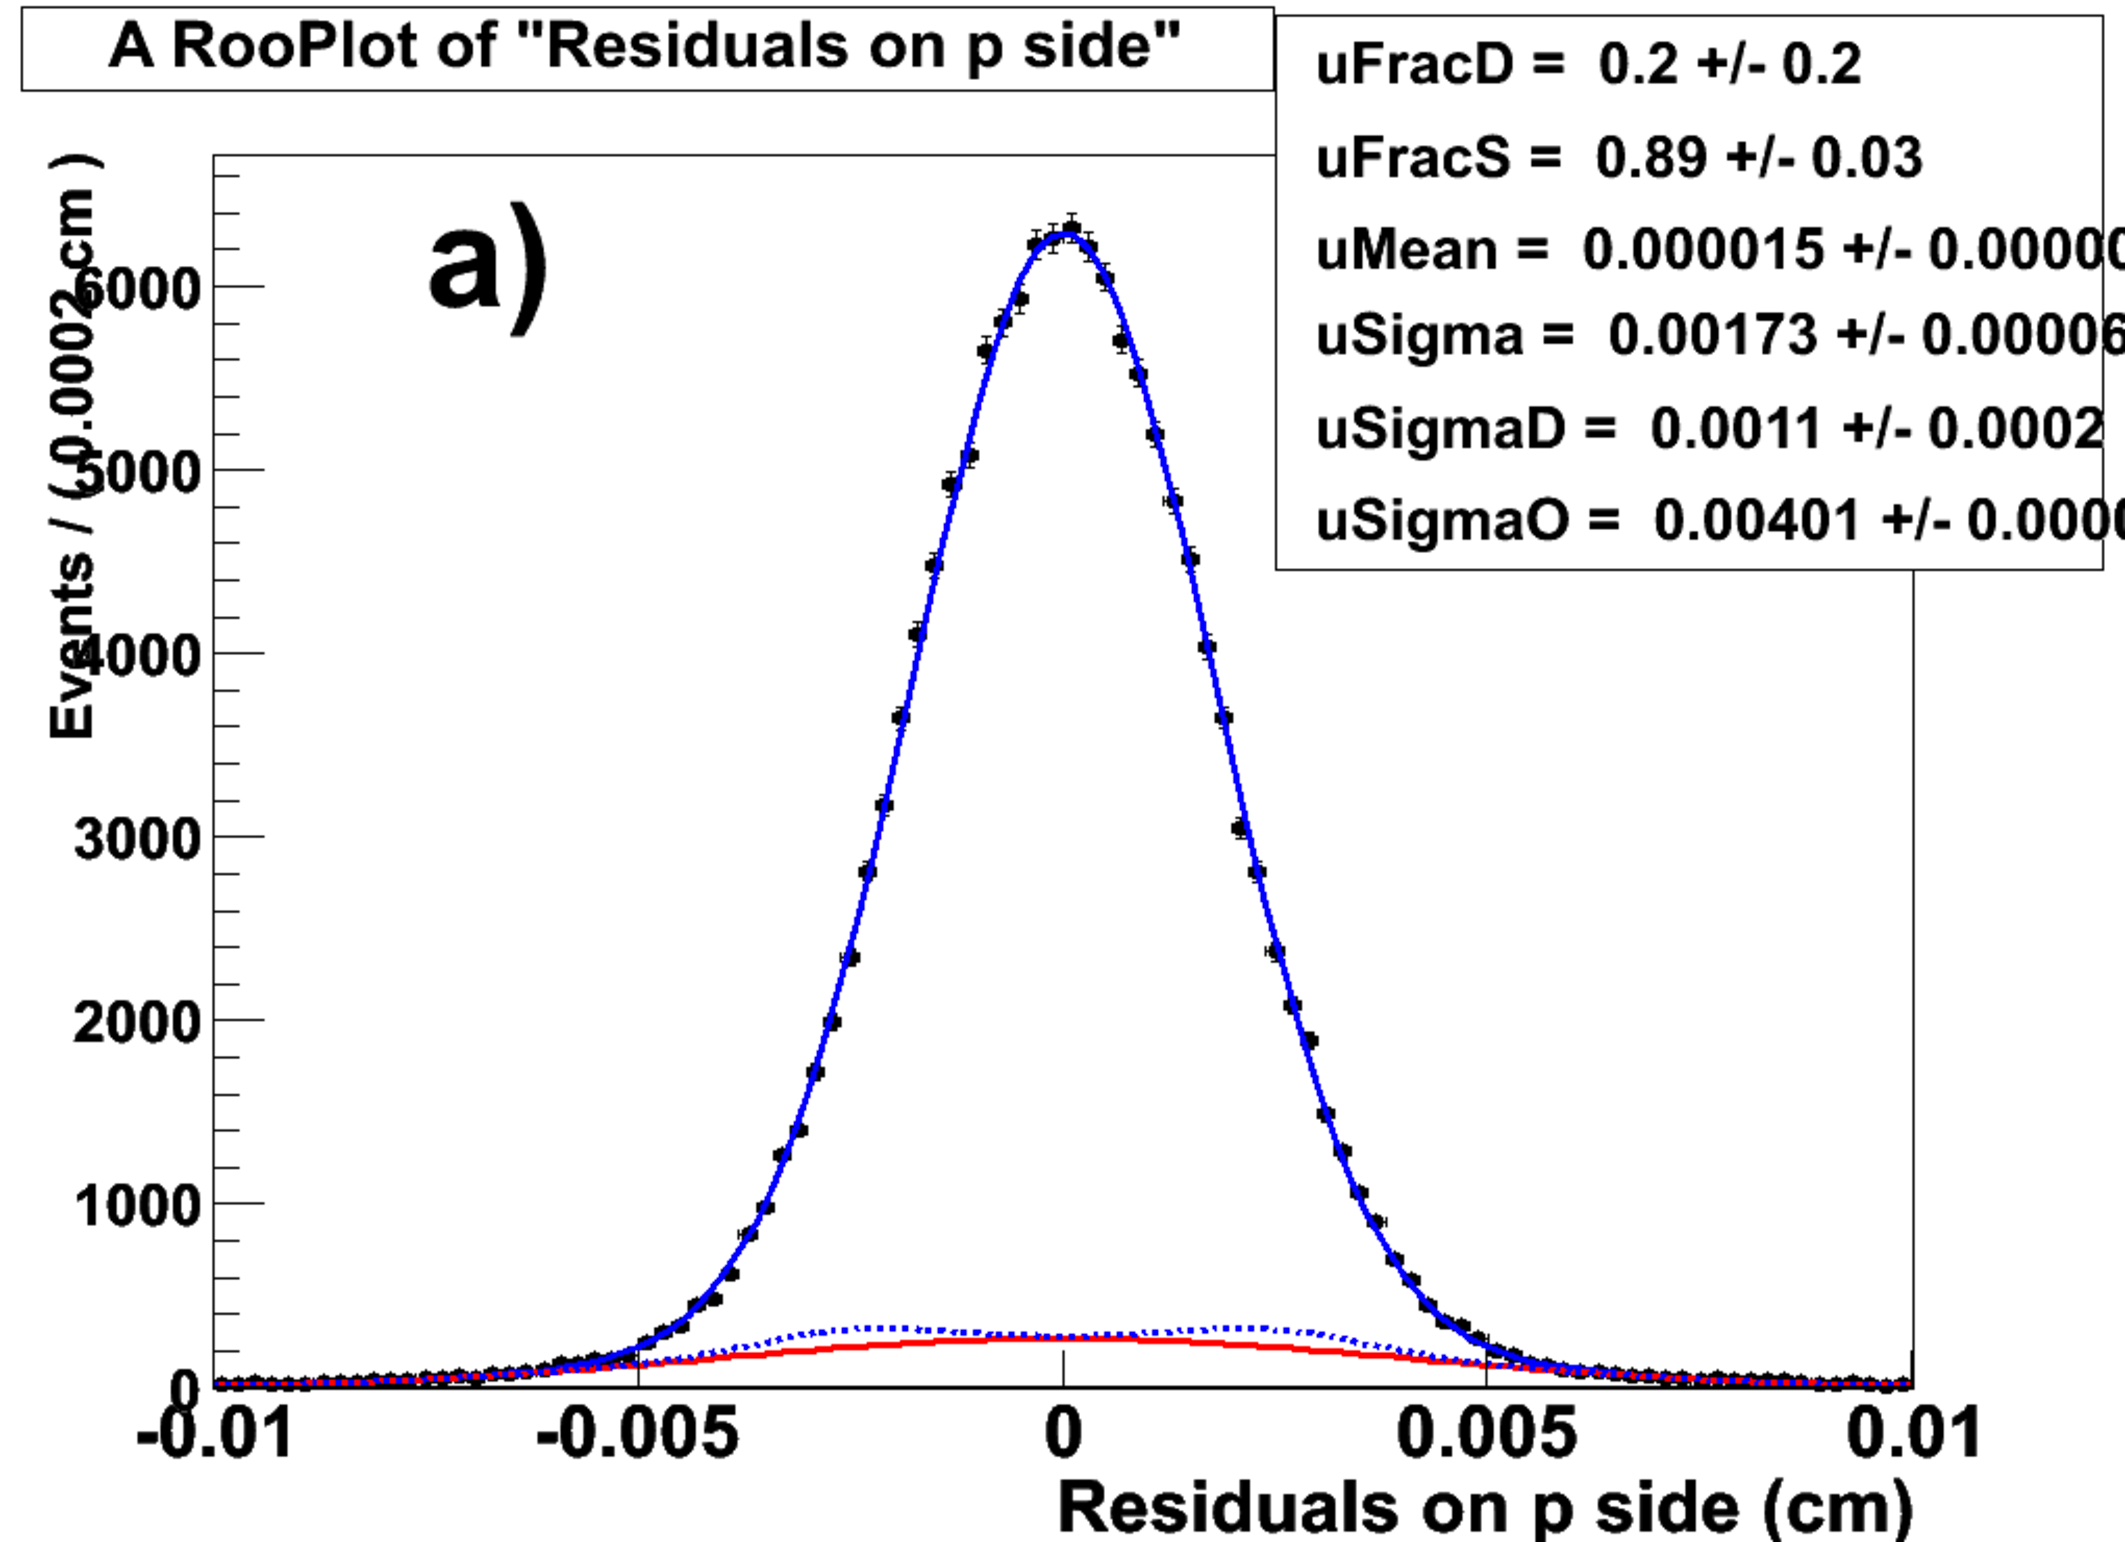
\includegraphics[width=0.39\textwidth]{res_pside_45deg.pdf}
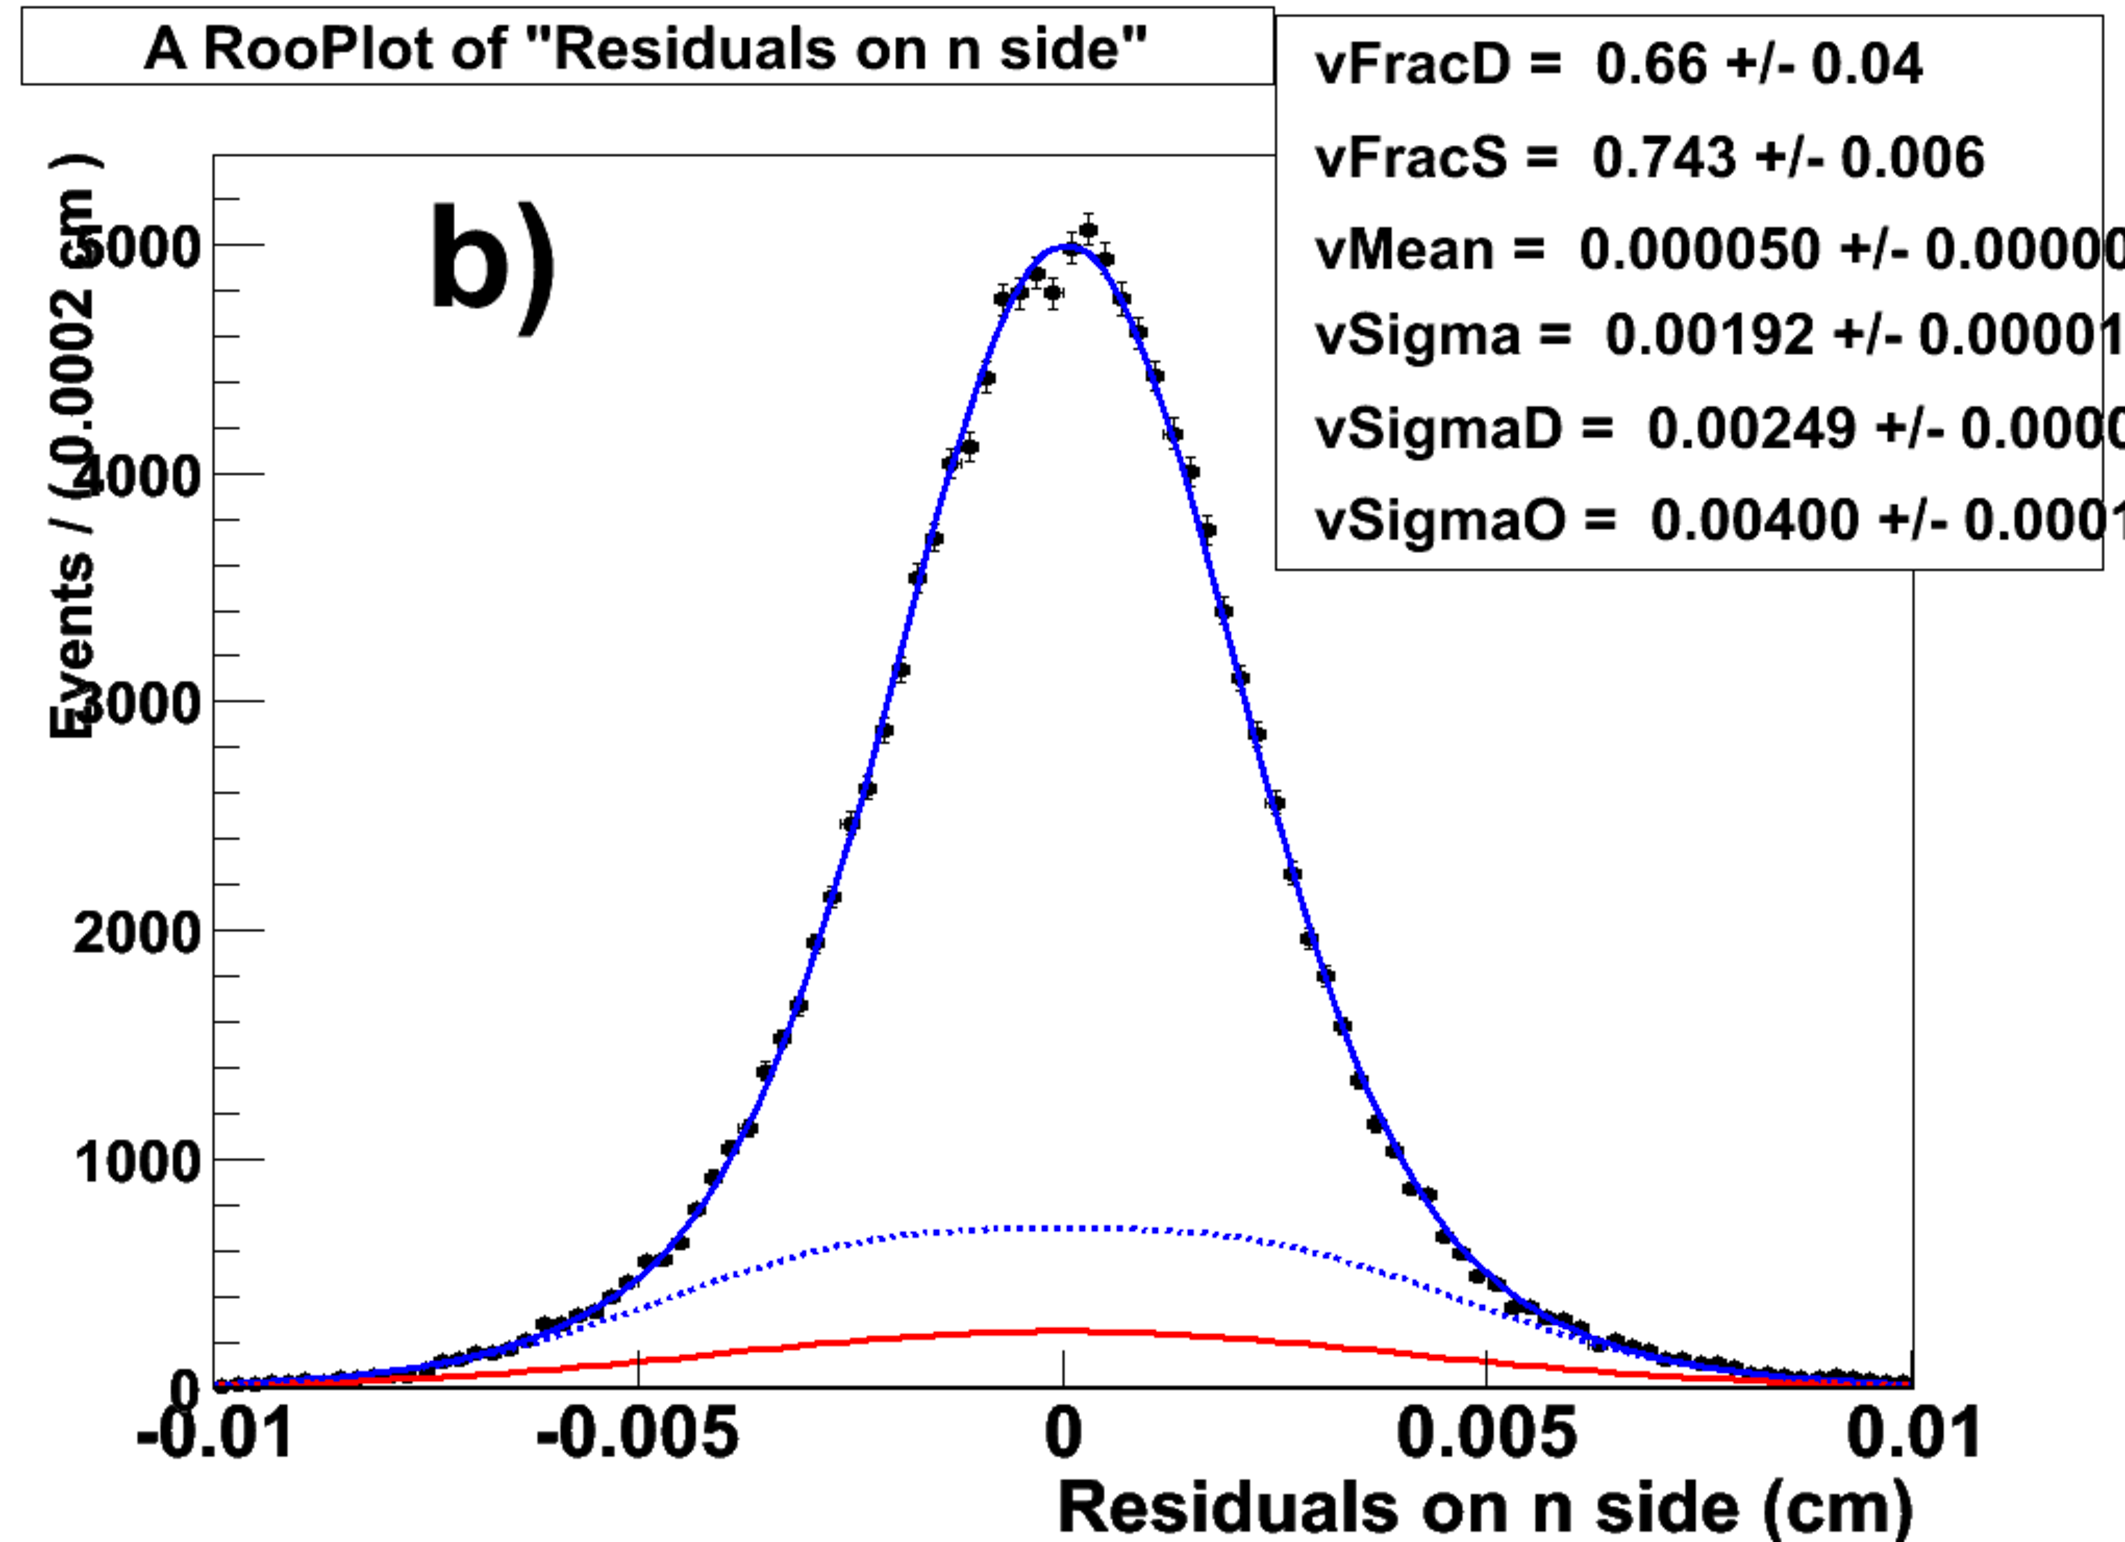
\includegraphics[width=0.39\textwidth]{res_nside_45deg.pdf}
\caption{\label{fig:res_angles}Residuals distribution of striplets detector at different incident track angle. From top to bottom raw the incident track angle was 5, 10, 20, 30 and 45$^{\circ}$. 
(a) is for $p-$side, (b) for $n-$side. Points are data, the fit function is given in Equation~\ref{eq:res_pdf}.}
\end{figure}

As it can be seen the contribution of the double peak Gaussian is less and less important as the 
angle increases; this is due to the charge sharing being more and more symmetric. This analysis 
confirmed the validity of the hypothesis about the influence of the threshold on the residuals 
distribution.


 \section{Summary and Discussion}
 \label{sec:Slim5Summary}
 
 Thin and excellent spatial resolution silicon detectors are mandatory to fulfil the physics program 
 of Super Flavour Factories and Linear Colliders. 
 The solutions proposed by the SLIM5 collaboration, the CMOS MAPS Apsel4D and the DSSD 
 striplets, proved to be an excellent starting point for the development of tracking and vertexing 
 detectors for those experiments. 
 
 Indeed they were both ``light'' in terms of material budget, 0.1\% and 0.2\% of $X_0$ for the 
 100~$\mu$m thick Apsel4D and for the striplets (sensor only but no readout electronics present in 
 the active area) respectively. The possibility for striplets to have the readout electronics outside 
 the active area made them the preferred option for the layer0 of the proposed SuperB SVT.
 Hit-efficiency was high and matched the expectations for both Apsel4D and striplets. The 
 Apsel4D chip hit efficiency was limited by the fill factor due to the competitive wells; 
 for the striplets no major showstopper was found and the efficiency was very close to 100\%.

 For what concerns 
 the space-point resolution, both detectors matched the expected performance for  50~$\mu$m pitch 
 detectors, 
 but they suffered for the low number of clusters with more than 1 cell and, more important, 
 from the high threshold. 
  
  Faster readout was in need for both solutions, even if FSSR2 chip was operated at up to 
  70~MHz.
  
 Smaller pitches and better noise control were needed to 
 match the specifications. In particular, as it was investigated throughly for striplets, zero suppression 
 impacts severely the spatial resolution if thresholds are relatively high and their effects are not 
 corrected for. 
 
 Research continued for CMOS MAPS~\cite{Rizzo:2013aza}, improving the efficiency by increasing 
 the fill factor, reducing the pitch to 40~$\mu$m and exploring vertical integration. 
 Striplets would have benefited from a new readout chip.

